\documentclass[a4paper,twoside,notoccite,tight,10pt]{report}
\usepackage{giuditta}
\usepackage[dvips]{graphicx}
\usepackage[undotted]{minitoc}
\usepackage{psfrag}
\usepackage[big]{layaureo}
\usepackage[bottom]{footmisc}
\usepackage[dvips]{hyperref}

\hypersetup{colorlinks=true,%
linkcolor=blue}
\hypersetup{pdftitle=Dispense di Relativita'}
\hypersetup{pdfauthor=Giovanni Lanzani}

\graphicspath{{./figure/}}
\mtcselectlanguage{italian}
\makeindex
\addtolength{\voffset}{1cm}
\setcounter{minitocdepth}{2}
\mtcsetfont{minitoc}{*}{\footnotesize\rmfamily\upshape\mdseries}
\mtcsetfont{minitoc}{section}{\footnotesize\rmfamily\upshape\bfseries}
%\includeonly{notestoriche}
\begin{document}
\dominitoc
\adjustmtc
\nocite{barone,marchetti,bettini}
\newcommand{\la}{\ensuremath{\Lambda}}
\newcommand{\f}{\ensuremath{F^{\mu\nu}}}
\newcommand{\ff}[2]{\ensuremath{\partial^{#1}A^{#2} - \partial^{#2}A^{#1}}}
\newcommand{\D}{\mathrm{d}}
\newcommand{\sq}{\sqrt{1-\frac{v^{2}}{c^{2}}}}
\newcommand{\cem}{\ensuremath{\mt{H}_{\rem{cm}}}}
\newcommand{\lab}{\ensuremath{\mt{H}_{\rem{lab}}}}
\setlength{\unitlength}{1mm}
\selectlanguage{italian}
\begin{titlepage}
\begin{center}
\mbox{} \vskip 2cm
\ \Huge \hskip 0.5cm Dispense di \enf{\Huge Istituzioni di Relativit\`a}\\
\vskip 2cm
\normalsize Dagli appunti presi alle lezioni del professor PierAlberto Marchetti\\
\vskip 3cm

 Corso di Istituzioni di Relativit\`a \\
\hskip 1.78cm per la Laurea Triennale in Fisica \newline
Facolt\`a di Scienze Matematiche Fisiche Naturali, Universit\`a di Padova \\
Anno Accademico 2005-2006\\
\vspace{1cm}


\end{center}
\end{titlepage}


Copyright \copyright  2006 GIOVANNI LANZANI. \newline
      Permission is granted to copy, distribute and/or modify this
      document \newline
      under the terms of the GNU Free Documentation License, Version 1.2 \newline
      or any later version published by the Free Software Foundation. \newline
      A copy of the license is included in the section entitled "GNU \newline
      Free Documentation License". \newline
\tableofcontents
\part{Il corso}
\chapter*{Introduzione}
\addcontentsline{toc}{chapter}{\numberline{}Introduzione}
\begin{flushright}
\enf{L'anima mia attende il Signore\\
Pi\`u che le sentinelle l'aurora.}
\end{flushright}

Questa dispensa \`e nata come pretesto per affinare le mie capacit\`a
con \LaTeX. Penso di aver raggiunto il mio scopo.

Era mia intenzione distribuirla gratuitamente, e per un periodo di tempo
\`e stato cos\`i. Poi cambiai opinione, e decisi di lavoravici per poi
venderla al prezzo di due pacchetti di Marlboro.

Voi che leggete non l'avete pagata, quindi ho evidentemente cambiato di
nuovo idea. Perch\'e? Be', i motivi sono tanti, il principale dei quali
\`e, probabilmente, la filosofia che sta dietro all'open source, motivo
per il quale ora, non solo la dispensa \`e gratuita, ma \`e anche
disponibile il suo codice sorgente (non azzardatevi a cambiare questa
pagina \dots)

\begin{wrapfigure}[10]{r}{4cm}
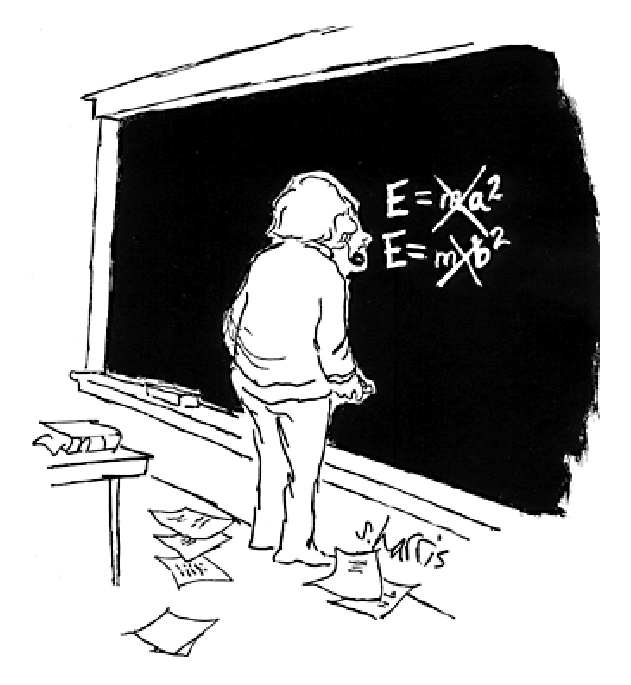
\includegraphics[width=3cm]{emcsquaredcartoon.eps}
\end{wrapfigure}

Ringrazio Alessandro Broggio per l'aiuto datomi nella stesura di questa
dispensa, il professor Zampieri e il professor Zilio, che m'hanno
accompagnato, chi pi\`u, chi meno, nel mondo della matematica e della
fisica, alle scuole superiori; inoltre ringrazio il professor Marchetti,
che s'\`e preoccupato di correggermi la dispensa, di fare la tesi con
me, e di tenere il corso, nonch\'e di favorire noi studenti di fronte ai
professori di laboratorio del C.C.S. di fisica, che cercano sempre di
rubare ore alle materie pi\`u belle. Il ringraziamento pi\`u grande va
poi a Giuditta, senza la quale non avrei scritto niente, essendo stata
lei a spingermi a continuare quando di voglia non ne avevo.

V'\`e poi la mia mail \emph{lanzani@spiro.fisica.unipd.it},\footnote{Ho
una ragazza, studio, sono in Erasmus in Olanda, da dove,
spero, non torner\`o: quindi non ho tutto il tempo libero che avete voi:
pazientate se non vi rispondo subito.} attiva per ricevere suggerimenti
che vi vengono alla mente, ed errori che riscontrate, nella lettura di
questa dispensa. \`E anche stata messa sotto cvs, ma la cosa non mi pare
abbia riscosso troppo successo, in quanto oltre a me nessuno l'ha mai
modificata. In ogni caso la potete trovare, coi sorgenti, su
\begin{center}
	http://spiro.fisica.unipd.it/$\thicksim$lanzani/public/rel/
\end{center}

 Una nota per tutti i computer nerd con mille suggerimenti stilistici:
cercate di concentrare le vostre energie nel correggere la ``sostanza''
della dispensa.

Parlando del corso: non preoccupatevi per la notazione tensoriale: sarebbero
necessari esercizi semplici per impratichirsi. Il resto \`e tutto
abbastanza facile, e, soprattutto bello. Forse potr\`a risultare ancora
pi\`u interessante leggere la mia tesi di laurea, che costituisce la
seconda parte della dispensa. Non \`e molto difficile, e penso che una
volta terminato il corso (ma anche prima), sarete perfettamente in grado
di apprezzarne il valore.

Il corso si conclude con un'ora di relativit\`a generale, durante la quale,
ovviamente, non s'\`e nemmeno avuto il tempo di farsi una vaga
idea di quello che \`e la relativit\`a generale, e perci\`o non la
riporto.

 \vskip 0.2cm
 \hskip 1cm Giovanni Lanzani

%#!simpdftex latex relativita.tex
\chapter{Note storiche}
\minitoc Come nasce la relativit\`a ristretta, altrimenti detta
speciale? Nasce dal tentativo, riuscito, di conciliare meccanica
newtoniana ed elettromagnetismo. Einstein stesso scrive a proposito:
\begin{quote}
  \enf{La teoria della relativit\`a nasce necessariamente, per la
    presenza di serie e profonde contraddizioni, dalle quali sembrava
    non ci fosse uscita. La forza della nuova teoria sta nella
    consistenza e semplicit\`a con cui risolve queste difficolt\`a,
    usando poche, ma convincenti, assunzioni.}
\end{quote}
Ma dove queste teorie, elettromagnetismo e meccanica, erano in
disaccordo? 
%Newton sosteneva l'esistenza di un tempo assoluto,
%omogeneo (un tempo uguale per tutti gli osservatori, e indipendente
%dal sistema di riferimento); affermava altres\`i che lo spazio era
%assoluto, omogeneo, ed isotropo. Il sistema di riferimento ideale era
%quello delle stelle, chiamato sistema di riferimento delle stelle
%fisse, che per le conoscenze di allora erano, appunto, considerate
%fisse.  \newline 
Sostanzialmente sembrava che non si trovasse un gruppo di sistemi di
riferimento in cui le leggi dell'elettromagnetismo avessero la stessa
forma, ovvero per avere una descrizione dei fenomeni fisica, sembrava
fosse necessario modificare le leggi dell'elettromagnetismo a seconda
del sistema di riferimento in cui ci si trovava.

Si ipotizz\`o dunque che fossero le leggi per passare da un sistema di
riferimento all'altro ad essere sbagliate, ma a questo punto si rendeva
necessario cambiare le leggi della meccanica da un sistema di
riferimento all'altro.

Prima di poter procedere \`e tuttavia necessario dare
una definizione precisa di sistema di riferimento, in maniera da
evitare errori o imprecisioni:
\begin{definizione}
  Un sistema di riferimento \`e l'insieme di un sistema di coordinate
  e di orologi, sincronizzati tra loro, in grado d'associare ad ogni
  evento un punto dello spazio e un istante di tempo. Un sistema di
  riferimento in cui ogni corpo non soggetto a forze \`e in quiete o
  in moto rettilineo uniforme \`e detto sistema di riferimento inerziale.
\end{definizione}
La definizione precisa di evento verr\`a data pi\`u avanti, per ora
possiamo prendere la nozione euristica che abbiamo di esso. Nei sistemi
di riferimento in moto a velocit\`a costante rispetto a quello delle
stelle fisse, le leggi della meccanica assumevano la stessa forma
tramite le trasformazioni (\ref{eq:trasformazioni}). Quindi la terra
poteva considerarsi un ottimo laboratorio, in quanto
l'accelerazione\index{accelerazione!terrestre} che essa aveva, rispetto
a tale sistema, poteva dirsi trascurabile. Questo era vero se, come
detto, per collegare due sistemi di riferimento si utilizzavano le
(\ref{eq:trasformazioni}). Pi\`u
precisamente, detti $S$ ed $S'$ i due sistemi inerziali, $S'$ in moto
con velocit\`a $\mathsf{v}$ rispetto ad $S$ (velocit\`a costante in
direzione e modulo), si aveva che, se
\begin{displaymath}
  t,\mathbf{x} \mbox{ coordinate in $S$} \qquad t',\mathbf{x}' \mbox{
    coordinate in $S'$ }
\end{displaymath}
allora
\begin{equation}
  \left\{\begin{array}{l}
      \mathbf{x}'=\mathbf{x}+\mathbf{\mathsf{v}}t\qquad
      (\dagger)\\
      t'=t\end{array}\right. \label{eq:trasformazioni}
\end{equation}
 Si aveva poi l'\enf{invarianza degli intervalli temporali}, ossia:
\begin{equation}
  \Delta t=\Delta t'\label{eq:invtempo}
\end{equation}
e degli \enf{intervalli spaziali}
\begin{equation}
  l = |\Delta\mathbf{x}| =
  |\Delta\mathbf{x}'|=l'\label{eq:invspazio}
\end{equation}  
Vi era poi il:
\begin{teorema}[di addizione delle velocit\`a]
  \index{teorema!di addizione delle velocit\`a}
  \begin{displaymath}
    \mathbf{v}'=\frac{\de}{\de t}\mathbf{x}'=\frac{\de}{\de
      t}\mathbf{x}+\mathbf{\mathsf{v}}=\mathbf{v}+\mathbf{\mathsf{v}}
  \end{displaymath}
\end{teorema}
Tale teorema si ottiene derivando ($\dagger$), ed esso asserisce che
non esiste una velocit\`a assoluta.  
%
\newline 
%
Come anticipato prima, tuttavia, con queste trasformazioni le leggi
dell'elettromagnetismo non potevano essere valide in tutti i sistemi di
riferimento. Vediamo come.
\section{L'etere e l'elettromagnetismo di Maxwell}
Prendiamo l'equazione delle onde elettromagnetiche:
\begin{displaymath}
  \left(\frac{1}{c^2}\cdot\frac{\partial^2}{\partial
      t^2}-\mathbf{\nabla}^2\right)\mathbf{E}(\mathbf{x},t)=0 \qquad
  \mbox{(al posto di $\mathbf{E}$ si pu\`o avere $\mathbf{B}$)};
\end{displaymath}
nell'800 ritenevano che $c$ fosse la velocit\`a della luce nell'etere
luminifero (che porta la luce). Perch\'e si parlava di etere? 
%
%\newline
%
Come prima accennato, le leggi dell'elettromagnetismo non avevano la
stessa forma in tutti i sistemi di riferimento, e quindi l'elegante
forma proposta da Maxwell era corretta solo in uno di questi
sistemi. Si ipotizz\`o questo sistema uguale al sistema di riferimento
delle stelle fisse, e lo si ribattezz\`o etere, il sistema in cui le
leggi di Maxwell erano vere senza bisogno di modifiche.
%Si era
%scoperto che le leggi dell'elettromagnetismo, se valide in un
%determinato sistema di riferimento inerziale $S$, non lo erano pi\`u
%in $S'$, sistema in moto a velocit\`a costante rispetto a $S$. 
Vedere che in altri sistemi di riferimento queste modifiche erano
necessarie, non \`e di difficile constatazione: si prenda infatti
un'onda elettromagnetica (che ha la stessa velocit\`a di propagazione
della luce) nel sistema $S$. Essa ha velocit\`a $c$, poich\'e per
l'elettromagnetismo la velocit\`a di propagazione di tale onda \`e
\begin{equation}
  c=\frac{1}{\sqrt{\mu_0\varepsilon_0}};
\end{equation}
se $S'$ si muove con velocit\`a $\rem{v}$ in direzione e verso
dell'onda elettromagnetica, esso rileva la luce avere velocit\`a
$c'=c-\rem{v}$, per il teorema appena visto. Ma allora non sarebbe pi\`u
valida la relazione (derivata dalle normali equazioni di Maxwell)
\begin{displaymath}
  c'=\frac{1}{\sqrt{\mu_0\varepsilon_0}}
\end{displaymath}
essendo $\mu_0$ e $\varepsilon_0$ costanti e \(c'\) la velocit\`a della
luce per l'osservatore di \(S'\). Se ne deduce che una, ed
una sola, delle seguenti ipotesi dev'essere vera:
\begin{description}
\item [Prima ipotesi] Le leggi della meccanica sono covarianti per
  cambiamento di sistema di riferimento inerziale, ma non lo sono le
  leggi dell'elettromagnetismo; le trasformazioni
  (\ref{eq:trasformazioni}) sono giuste.
\item [Seconda ipotesi] Le leggi della meccanica e
  dell'elettromagnetismo sono covarianti per cambiamento di sistemi di
  riferimento inerziale, le trasformazioni (\ref{eq:trasformazioni})
  sono giuste, ma il modo in cui sono scritte le leggi
  dell'elettromagnetismo \`e sbagliato.
\item [Terza ipotesi] Le leggi della meccanica e
  dell'elettromagnetismo sono covarianti per cambiamento di sistemi di
  riferimento inerziale, il modo in cui sono scritte le leggi
  dell'elettromagnetismo \`e giusto (si lascia dunque spazio ad
	    un'eventuale riscrittura delle leggi della meccanica), ma le
	    trasformazioni
  (\ref{eq:trasformazioni}) sono sbagliate.
\end{description}
L'ipotesi corretta la avanz\`o Einstein, e verr\`a affrontata dopo. 
%Se
%l'ipotesi giusta fosse la seconda, esisterebbe un sistema privilegiato,
%quello in cui le onde si propagano con velocit\`a $c$; in tale sistema,
%detto etere, sarebbero valide le equazioni di Maxwell; si pensava tale
%sistema fosse il sistema di riferimento delle stelle fisse.

Nelle tre ipotesi abbiamo fatto uso del termine ``covarianti'':
cosa significa? Una legge fisica \`e covariante quando ha la stessa
forma per tutti i sistemi di riferimento inerziali; ad esempio nel
sistema di riferimento $S$ la seconda legge
di Newton si scrive 
\begin{displaymath}
 \bef{F} = m\bef{a}; 
\end{displaymath}
cambiando sistema di riferimento, sar\`a necessario usare delle
trasformazioni di coordinate per poter scrivere la legge nel nuovo
sistema; ebbene, usando le trasformazioni di Galileo e le leggi della
meccanica conosciute, nel nuovo sistema di riferimento la
``trasformazione'' della seconda legge di Newton \`e
\begin{displaymath}
  \bef{F'} = m'\bef{a'},
\end{displaymath}
dove \(m = m'\): dunque la legge della meccanica ha la stessa forma in
entrambi i sistemi di riferimento, e si pu\`o parlare di covarianza.

%Come sopra detto, $c$ era la velocit\`a della luce in tale sistema. La
%domanda che a quel tempo ci si poneva era: 

Assumendo dunque che l'esistenza dell'etere, era possibile trovare il
moto della terra rispetto a tale sistema?  Vediamo ora due esperimenti
che rispondono a tale domanda in maniera inconciliabile.
\subsection{Esperimento sull'aberrazione}
\index{aberrazione} \setlength{\unitlength}{0.7mm}
\begin{wrapfigure}[17]{r}{4cm}
  \begin{picture}(50,75)
    \put(5,5){\line(1,0){40}}\multiput(25,5)(0,10){7}{\line(0,1){5}}
    \put(22,70){\Huge$\star$} \put(20,5){\line(0,1){25}}
    \put(20,30){\line(1,0){10}}\put(30,30){\line(0,-1){25}}
    \put(28,5){\dashbox{2}(10,25){}}\put(30,17){\huge$\rightarrow$}
    \put(32,21){v}
  \end{picture}
  \caption{Luce stellare incidente sul telescopio}
  \label{fig:telescopio}

\end{wrapfigure}
\setlength{\unitlength}{1mm} Consideriamo il telescopio in figura
\ref{fig:telescopio}. Ci proponiamo di andare a verificare l'angolo di
inclinazione che esso deve avere per poter osservare la luce
proveniente da un corpo celeste. Se la terra si muovesse con una certa
velocit\`a rispetto a tale stella, le cose andrebbero come in figura,
e il telescopio, senza alcun angolo di inclinazione, sarebbe
inservibile. Infatti da quando il raggio della stella entra nel
telescopio, a quando raggiunge l'ordinata dell'obbiettivo
(consideriamo la stella, qualsiasi essa sia, solidale all'etere), il
telescopio si sposta e la luce non colpisce l'obbiettivo. Quindi \`e
necessario inclinare il telescopio. Chiamiamo l'angolo di inclinazione
$\vartheta$ (\`e l'angolo formato dalla terra e dal lato pi\`u corto
dell'obbiettivo). Per valutare approssimativamente la velocit\`a della
terra rispetto al sistema delle stelle fisse, consideriamo il sole
come una stella fissa; la distanza terra sole vale
$R_{\scriptscriptstyle TS}= \unit[150\cdot10^9]{m}$. Il periodo di
rivoluzione attorno al sole vale
$T=\unit[365]{d}\Longrightarrow\mathsf{v}=3\cdot10^4\rem{m}/\rem{s}$.
Se il telescopio \`e lungo $l$ (fare un disegno per capire meglio),
il tempo di percorrenza della luce \`e $t=l \cos \vartheta /c$. La
distanza percorsa dal telescopio in $t$ \`e $x=\mathsf{v}t$.  L'angolo
$\vartheta$ risulta dunque:
\begin{displaymath}
  \tan\vartheta= \frac{\mathsf{v} t}{l \cos \vartheta} =
  \frac{\mathsf{v}t}{ct}\approx10^{-4}
\end{displaymath}
Come si vede quest'angolo \`e molto piccolo, ma le misure sono in
accordo con la teoria, cio\`e \`e effettivamente necessario inclinare
i telescopi di $\vartheta$ per poter osservare i corpi
celesti.\footnote{Tuttavia quest'esperimento non fu considerato
  decisivo, poich\'e esso utilizzava le approssimazioni di ottica
  geometrica dell'elettromagnetismo.}
\subsection{L'esperimento di Michelson e Morley}
\index{Michelson-Morley, esperimento di}L'esperimento di Michelson e
Morley, effettuato per la prima volta nel 1881, era stato ideato per
trovare la velocit\`a della luce rispetto all'etere.  L'esperimento
\`e schematizzato in figura \vref{fig:mm}.
\setlength{\unitlength}{0.5mm}
\begin{figure}[htb]
  \begin{center}
    \begin{picture}(110,100)
      \put(5,50){\vector(1,0){65}}\put(60,40){\line(1,1){20}}
      \put(70,50){\vector(0,1){30}} \put(14,37){\tiny Specchio
        semi-rifrangente}
      \put(60,80){\line(1,0){20}}\multiput(60,80)(5,0){5}{\line(1,3){3}}
      \put(70,80){\vector(0,-1){30}}\put(70,50){\vector(1,0){30}}
      \put(100,40){\line(0,1){20}}
      \multiput(100,40)(0,5){5}{\line(3,1){8}}
      \put(70,50){\vector(0,-1){30}} \put(60,63){\vector(0,-1){13}}
      \put(55,64){$L$} \put(60,67){\vector(0,1){13}}
      \put(83,40){\vector(-1,0){13}}\put(87,40){\vector(1,0){13}}
      \put(85,62){\tiny Specchio} \put(84,37){$L$} \put(83,80){\tiny
        Specchio} \put(5,55){\tiny Sorgente}
      \put(66.5,14.5){\Huge$\blacksquare$} \put(62,8){\tiny
        Rilevatore} \put(3,45.8){\Huge$\blacktriangleright$}
    \end{picture}
    \caption{Schema dell'esperimento di Michelson e Morley, visto nel
      sistema di riferimento solidale alla terra} \label{fig:mm}
  \end{center}
\end{figure}
Spieghiamo cosa succede. La terra si muove con velocit\`a $\mathsf{v}$
rispetto all'etere (secondo le convinzioni dell'epoca). Dunque i raggi
che colpivano lo specchio semirifrangente, e si propagavano in
direzione verticale, facevano un percorso, nel sistema di riferimento
etere, come quello in figura \vref{fig:mim1} (tener ben presente il
fatto che una volta raggiunto uno specchio, la luce si propaga come
un'onda emisferica).
\begin{figure}[htb]
  \begin{center}
    \begin{picture}(50,65)
      \put(10,10){\vector(1,3){15}}\put(10,10){\line(1,0){15}}
      \multiput(25,10)(0,10){5}{\line(0,1){5}}
      \put(10,55){\line(1,0){30}}\put(25,55){\vector(1,-3){15}}
      \put(35,5){\line(1,1){10}}
      \multiput(10,55)(5,0){7}{\line(1,3){3}} \put(30,50){\tiny
        Specchio}\put(42,8){\tiny Specchio
        semi-rifrangente}\put(17.5,5){$\mathrm{v}t$} \put(22,25){$l$}
      \put(13,36){$ct$}
    \end{picture}
    \caption{Percorso della luce in direzione verticale}
    \label{fig:mim1}
  \end{center}
\end{figure}
Dal disegno si capisce (\`e sufficiente usare il teorema di Pitagora)
che $(ct)^2=l^2+(\mathsf{v}t)^2$, da cui risulta:
\begin{equation}
  t_{\perp}=2t=\dfrac{2l}{c}\dfrac{1}{\sqrt{1-\dfrac{\mathsf{v}^2}{c^2}}}.
  \label{eq:mim1}
\end{equation}
L'altro raggio invece fa il percorso, nell'etere, in figura \ref{fig:mim2}. \setlength{\unitlength}{1mm}
\begin{figure}[!h]
  \begin{center}
    \begin{picture}(65,28) \put(7.5,7.5){\line(1,1){10}}
      \put(6,18){\scriptsize Specchio
        semirifrangente}\put(12.5,12.5){\line(1,0){36}}
      \put(27.5,12.5){\vector(1,0){8}}
      \put(27.5,12.5){\vector(-1,0){5}} \put(48.5,2.5){\line(0,1){20}}
      \multiput(48.5,2.5)(0,4){6}{\line(1,1){5}}
      \put(12.5,12.5){$\underbrace{\makebox[36mm][c]{}}$}
      \put(29,7){$L$}\put(57,12.5){Specchio}
    \end{picture}
    \caption{Percorso della luce in direzione orizzontale}
    \label{fig:mim2}
  \end{center}
\end{figure}
Si pu\`o facilmente capire che
$t_{\sslash}=\frac{l}{c-v}+\frac{l}{v+c}$, da cui:
\begin{equation}
  t_{\sslash}=\dfrac{2l}{c}\cdot\dfrac{1}{1-\frac{\mathsf{v}^2}{c^2}}
  \label{eq:mim2}
\end{equation}
Dal momento che $ \mathsf{v} \ll c $ possiamo sviluppare in serie di $v^2 / c^2$
la (\ref{eq:mim1}) e la (\ref{eq:mim2}), ottenendo:
\begin{equation}
  t_{\perp}=\frac{2l}{c}\left(1+\frac{1}{2}\frac{\mathsf{v}^2}{c^2}\right)
\end{equation}
\begin{equation}
  t_{\sslash}=\frac{2l}{c}\left(1+\frac{\mathsf{v}^2}{c^2}\right)
\end{equation}
In definitiva $t_{\sslash} -
t_{\perp}\simeq\frac{\mathsf{v}^2l}{c^3}$. Sempre facendo riferimento
alla figura \vref{fig:mm}, si vede che i raggi, dopo esser tornati
indietro, interferivano. Con un interferometro (il rivelatore della
figura), si poteva misurare quest'interferenza. Lo sfasamento
spaziale, in termini di lunghezza d'onda, \`e:

\begin{displaymath}
  \Delta\lambda=c(t_{\sslash}-t_{\perp})\simeq\frac{\mathsf{v}^2l}{c^2}
\end{displaymath}


Il numero di frange che si doveva dunque rilevare con l'interferometro
era:
\begin{displaymath}
  \frac{\Delta n}{n} = 
  \frac{\Delta\lambda}{\lambda}=\frac{l}{\lambda}\frac{\mathsf{v}^2}{c^2}
\end{displaymath}
L'esperimento del 1887 (quello eseguito con i migliori accorgimenti
per diminuire gli errori di misura), aveva $l=\unit[11]{m}$,
$\lambda=\unit[6\cdot10^{-7}]{m}$, $v=10^{-4}c$. Da questi dati
risulta $\Delta n / n =0.18 \pm 0.01$. Tuttavia i risultati
sperimentali davano $\Delta n < 0.01$, e  questo fatto rimaneva inspiegabile:
l'etere si muoveva con la terra? Come era possibile interpretare tale
fenomeno?
\begin{observazione}[Fitzgerald e Lorentz] Una prima risoluzione del
  problema fu avanzata da Fitzgerald (1889), il quale asseriva che il
  braccio parallelo alla direzione del moto, si contraeva di un
  fattore $\sqrt{1-\mathsf{v}^2/c^2}$. Poi venne Lorentz, che
  afferm\`o che, nel caso fosse vera la contrazione di Fitzgerald,
  allora anche i tempi del sistema in moto rispetto all'etere dovevano
  dilatarsi dello stesso fattore $\sqrt{1-\mathsf{v}^2/c^2}$. In tal
  modo egli trova le trasformazioni tra i sistemi di riferimento che
  portano il suo nome (e che andremo a ricavare dopo).
\end{observazione}
\section{Princ\`ipi di relativit\`a}
Successivamente la cosa venne affrontata da un punto di vista
matematico: tra il 1902 e il 1905, Poincar\'e si avvicin\`o al
principio di relativit\`a einsteniano, dicendo:
\begin{principio}[di relativit\`a di Poincar\'e]\index{principio di
    relativit\`a!di Poincar\'e}
  Le leggi della fisica devono essere covarianti (avere cio\`e la
  stessa forma) per sistemi inerziali.
\end{principio}
Poincar\'e trov\`o dunque le trasformazioni di coordinate che resero
l'elettrodinamica compatibile con il principio di relativit\`a. Tali
trasformazioni sono le trasformazioni di Lorentz, che costituiscono un
gruppo; tale gruppo pu\`o essere ampliato ulteriormente, mantenendo la
sua struttura, dando origine al gruppo di Poincar\'e.

Venne poi la volta di Einstein (1905), il quale pose alla base della
sua teoria due principi:
\begin{dinglist}{192}
\item Principio di relativit\`a
\end{dinglist}
\begin{dinglist}{193}
\item La velocit\`a della luce \`e uguale in tutti i sistemi di
  riferimento inerziali
\end{dinglist}
Quale fu la grande innovazione di Einstein rispetto a Poincar\'e?  Il
fatto che egli elimin\`o il concetto di etere.\footnote{Ad inizio
  capitolo abbiamo imbrogliato il lettore, dicendo che la relativit\`a
  ristretta nasce per i contrasti tra elettromagnetismo e meccanica:
  Einstein, nello sviluppare la sua teoria, venne invece mosso dalla
  convinzione che non potesse esistere un sistema di riferimento
  privilegiato, ovvero di un moto assoluto, che portasse delle
  asimmetrie nell'elettromagnetismo; che questo risolvesse i contrasti
  di cui abbiamo parlato \`e un altro discorso, poich\'e non era
  possibile risolvere il dilemma di Einstein senza appianare i
  contrasti tra meccanica ed elettrodinamica.}


Successivamente, dall'invarianza di $c$, Einstein, con una serie di
esperimenti ideali, ricav\`o tutta una serie di leggi, tra cui le
trasformazioni di Lorentz. Cominciamo con lo scrivere gli assiomi alla
base della sua teoria.
\begin{dinglist}{202}
\item Omogeneit\`a e assolutezza dello spazio e del tempo, e isotropia
  (non vi sono differenze tra le direzioni) dello spazio. \footnote{In
    realt\`a questo primo assioma era implicito nella sua trattazione}
\end{dinglist}
\begin{dinglist}{203}
\item Si ha l'equivalente del principio di relativit\`a di Poincar\'e:
  \begin{principio}[di relativit\`a einsteniano]\index{principio di
      relativit\`a!di Einstein} Le leggi della
    fisica hanno la stessa forma in tutti i sistemi inerziali.
  \end{principio}
\end{dinglist}
\begin{dinglist}{204}
\item La velocit\`a della luce nel vuoto\footnote{Ossia assenza di
    materia} \`e la stessa in tutti i sistemi di riferimento inerziali
\end{dinglist}
\begin{osservazione}
  Osserviamo che \ding{202} era valido anche prima della teoria della
  relativit\`a di Einstein
\end{osservazione}
\begin{osservazione}
  Nella fisica pre-relativistica \ding{203} era sostituito dal
  principio di \emph{relativit\`a galileiano}, il quale asseriva:
\end{osservazione}
\begin{principio}[di Relativit\`a di Galileo]\index{principio di
    relativit\`a!di Galileo} Le leggi della meccanica hanno la stessa
  forma in tutti i sistemi inerziali.\footnote{Come gi\`a notato,
    ci\`o era impossibile per l'elettromagnetismo, se si usavano le
    trasformazioni di Poincar\'e.}
\end{principio}
\begin{osservazione}
  In fisica pre-relativistica \ding{204} era sostituita
  dall'invarianza degli intervalli spaziali (\ref{eq:invspazio}) e
  temporali (\ref{eq:invtempo})
\end{osservazione}

\chapter{Relativit\`a Einsteniana}
\minitoc
% Einstein affermava che $c$ era una costante universale. Osservando
% che $x$ e $ct$ hanno le stesse unit\`a di misura, si potrebbe
% asserire che non sono pi\`u $\Delta x$ e $\Delta t$ ad essere
% invarianti, bens\`i:
% \begin{equation}
%(\Delta s)^2 = (c\,\Delta t)^2-\Delta x^2. \label{eq:invariante}
%\end{equation}
%Che ci\`o sia invariante lo dimostreremo pi\`u avanti.
Einstein a questo punto si premura di costruire il suo sistema basato
su \ding{202}, \ding{203}, \ding{204}. Come comincia? Prendiamo una
sbarra lunga $l$ in un sistema di riferimento inerziale, che chiamiamo
$S$. Per prima cosa Einstein asserisce che assumere che ogni sistema
di riferimento inerziale veda la sbarra lunga $l$ non \`e, a priori,
un'ipotesi giustificata. Come si misura la lunghezza in moto? Per
concretizzare prendiamo una sbarra $\overline{PQ}$, solidale con il
sistema $S$, il quale si muove con velocit\`a $\mathbf{\mathsf{v}}$
rispetto al sistema $S'$; l'osservatore della sbarra misura la
lunghezza della sbarra con un metro (la sbarra \`e ferma rispetto a
lui); l'osservatore in $S'$ pu\`o fotografare la sbarra e misurare la
fotografia, di modo che gli estremi $P$ e $Q$ siano osservati allo
stesso istante nel suo sistema di riferimento. Si ha che 
\begin{displaymath}
\begin{array}{l} S' \mbox{ dice che la sbarra misura } l'\\
  S \mbox{ dice che la sbarra misura } l \end{array}
\end{displaymath}

Einstein afferma che nulla, dal punto di vista logico, mi garantisce
$l=l'$. Quindi non \`e affatto detto che le misure di lunghezza
rimangano inviariate passando da un sistema di riferimento all'altro.
\section{Glory \& Consequences}
Diamo innanzi tutto la definizione di evento:
\begin{definizione}
  Gli eventi, dal punto di vista fisico, sono le minime determinazioni
  spazio-temporali possibili; un evento, nei diagrammi
  spazio-temporali \`e rappresentato da tre coordinate spaziali
  (saranno $(x^1,x^2,x^3)$), e una coordinata temporale (sar\`a
  indicata come $x^0$).%
  \footnote{Dato che non sono capace di disegnare
    in 4D, e d'altronde voi non siete capaci di vedere in 4D
    (eccetto Candilera), sopprimiamo dai nostri disegni le altre due
    coordinate spaziali, con le quali siamo abituati a trattare.}
\end{definizione}
La metrica spazio-temporale per questi eventi sar\`a
\begin{equation}
  \label{eq:invariante}
  \de s^2 = \de t^2 - \de \bef{x}^2
\end{equation}
Prendiamo in considerazione un diagramma (vedi figura
\ref{fig:diagramma1}) dove come ascisse abbiamo le $x$, e come
ordinate abbiamo $ct$. I diagrammi che andremo a considerare
descriveranno dunque lo spazio-tempo, assumendo che esso sia una
variet\`a differenziale a 2 (o a 4) dimensioni \footnote{Ovvero esso
  \`e continuo, differenziabile, con topologia localmente omeomorfa ad
  $\mathbb{R}^2$, o $\mathbb{R}^4$, separabile, con base di intorni
  numerabile (e pu\`o perci\`o essere metrizzabile).}. Tali diagrammi,
detti diagrammi di Minkowski\index{Minkowski!diagrammi di},
rappresentano lo spazio quadridimensionale con la metrica data dalla
(\ref{eq:invariante}), e questo spazio fornito di tale metrica \`e
detto spazio di Minkowski\index{Minkowski!spazio di}. In questo
diagramma tutti i raggi di luce che vi vengono rappresentati, sono
inclinati di $45^{\circ}$, poich\'e $c = x / t$. La traiettoria del
fascio di luce deve quindi essere la bisettrice tra asse spaziale ed
asse $ct$.\footnote{Come conseguenza del fatto che la velocit\`a della
  luce \`e uguale in tutti i sistemi.} Consideriamo un corpo~$A$ e un
corpo~$B$. L'origine sia $O$. $A$ e $B$ abbiano distanze uguali
rispetto ad $O$. Si faccia riferimento alla figura
\ref{fig:diagramma1}

\begin{figure}[htbp]
  \begin{center}
    \psfrag{ct}{$ct$} \psfrag{A}{$A$} \psfrag{B}{$B$} \psfrag{O}{$O$}
    \psfrag{x}{$x$}
    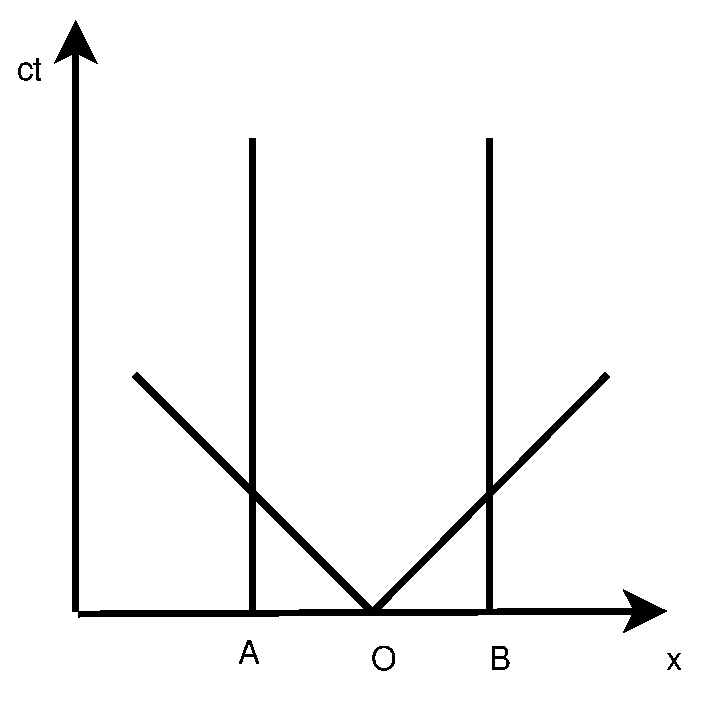
\includegraphics[height=7cm]{diagramma1.eps}
    \caption{Traiettoria di due punti fermi colpiti da un raggio di
      luce} \label{fig:diagramma1}
  \end{center}
\end{figure}
Se i due corpi sono fermi le loro traiettorie sono rette parallele a
$ct$. Un raggio di luce che parte da $O$, li colpisce allo stesso
istante se $\overline{AO}=\overline{OB}$, come gi\`a assunto. Cambiamo
ora le cose. Siano i due corpi in moto con velocit\`a
$\mathbf{\mathsf{v}}$ rispetto ad $S$ (siano cio\`e solidali ad un
sistema $S'$). %Si ha che valgono le (\ref{eq:trasformazioni}).

\begin{figure}[htbp]
  \begin{center}
    \psfrag{ct}{$ct$} \psfrag{ct'}{$ct'$} \psfrag{A}{$A$}
    \psfrag{B}{$B$} \psfrag{O}{$O$} \psfrag{A'}{$A'$}
    \psfrag{B'}{$B'$} \psfrag{x'}{$x'$} \psfrag{x}{$x$}
    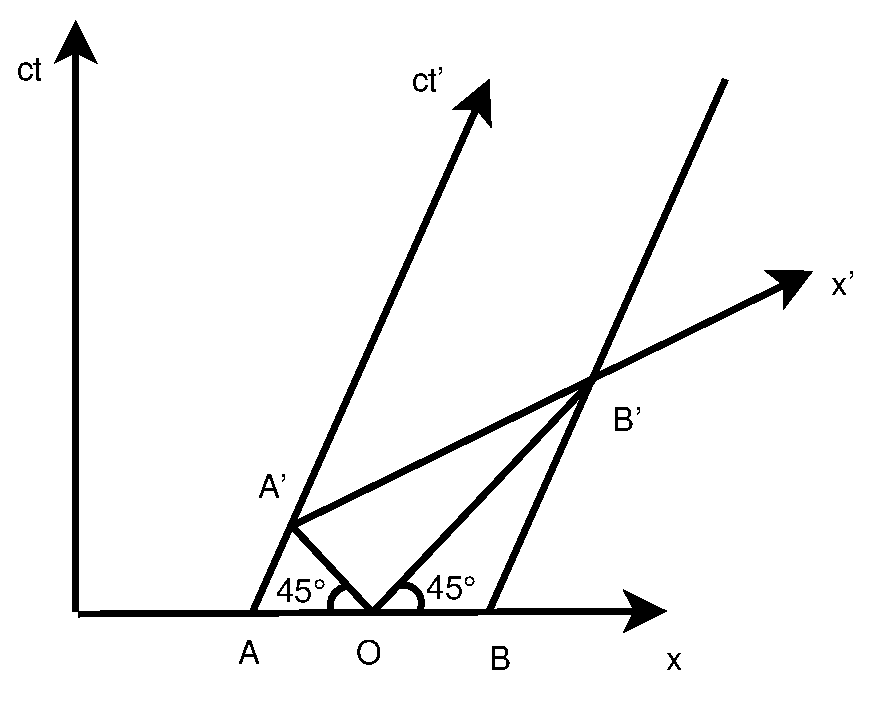
\includegraphics[height=7cm]{diagramma2.eps}
    \caption{Traiettoria di due punti in movimento colpiti da un
      raggio di luce} \label{fig:diagramma2}
  \end{center}
\end{figure}
Facendo riferimento alla figura \vref{fig:diagramma2}, siano $A'$ e $
B' $ solidali a $ S' $, immagini di $A$ e $B$ t.c. $ \overline{ AO } =
\overline{ OB } $.  Per $ S' $ la situazione \`e uguale a quella vista
in precedenza, e dunque gli aventi $ A' $ e $ B' $ sono simultanei in
$ S' $; infatti la luce interseca la linea di universo di $ A' $ e di
$ B' $ (che sono le stesse di $ A $ e $ B $, ma ritorneremo su questo
nel paragrafo \vref{assoluto}) nello stesso $ t' $ (usando \ding{203}
e \ding{204}). In $ S' $, tuttavia i due eventi non sono pi\`u
simultanei (basta proiettarli sull'asse $ ct $ per
accorgersene). Allora:
\begin{osservazione}
  Eventi contemporanei in un sistema possono non esserlo in un altro
  sistema.
\end{osservazione}
\section{Le trasformazioni di Lorentz}
Riprendiamo il discorso del capitolo precedente da un punto di vista
algebrico. Come prima sia $S'$ sistema di riferimento inerziale in
moto con velocit\`a $\mathbf{\mathsf{v}}$ rispetto ad $S$. Tempi e
moti con gli apici si riferiscono ad $S'$; senz'apici ad $S$.

Consideriamo la traiettoria di un moto fermo in $S'$: $x'=x_{0}'$,
indipendentemente da $t'$. Tale moto in $S$ soddisfer\`a la relazione
$x-\mathsf{v}t=x_{0}$, con $x_{0}$ indipendente da~$t$.  Allora,
dacch\'e $x_{0}$ e $x_{0}'$ sono costanti rispetto a~$t$, si pu\`o
scrivere:
\begin{equation}
  \frac{x-\mathsf{v}t}{x'}=\alpha \quad\mbox{ costante.}
  \label{eq:lore1}
\end{equation}
Da qui ricavo $\alpha x'=x-\mathsf{v}t$. Per reciprocit\`a, scambiando
$S$ con $S'$ e $\mathsf{v}$ con $-\mathsf{v}$, ottengo:
\begin{equation}
  \frac{x'+\mathsf{v}t'}{x}=\alpha \label{eq:lore2}
\end{equation}
Combinando la (\ref{eq:lore1}) con la (\ref{eq:lore2}), in modo da
eliminare $x'$:
\begin{equation}
  t'=\frac{1}{\alpha}\left(t+\frac{\alpha^2-1}{\mathsf{v}}x\right)
  \label{eq:lore3}
\end{equation}
Se impongo che $t=t'$ ottengo $\alpha=1$ e $x'=x-\mathsf{v}t$.
Tuttavia per avere la relativit\`a ristretta non devo imporre
$\alpha=1$, bens\`i $c=\mathrm{costante}$, cio\`e $x'=ct'$ e
$x=ct$. Sostituendo quest'ultime relazioni dentro (\ref{eq:lore1}) e
dentro (\ref{eq:lore2}) ottengo:
\begin{displaymath}
  \alpha c t'=ct-\mathsf{v}t
\end{displaymath}
\begin{displaymath}
  \alpha ct=ct'+\mathsf{v}t'
\end{displaymath}
Facendo il prodotto tra le due ottengo
\begin{displaymath}
  \alpha=\pm \sqrt{1-\frac{\mathsf{v}^2}{c^2}}
\end{displaymath}
Dacch\'e per $v=0$ si ha $\alpha=1$, alla fin fine:
\begin{displaymath}
  \alpha=\sqrt{1-\frac{\mathsf{v}^2}{c^2}}
\end{displaymath}
Posso dunque ricavare le equazioni
\begin{displaymath}
  \left\{\begin{array}{l}
      x'=\frac{x-\mathsf{v}t}{\sqrt{1-\frac{\mathsf{v}^2}{c^2}}}\qquad
      \mbox{
        (deriva da (\ref{eq:lore1}))}\\
      \mbox{ }\\
      t'=\frac{t-\frac{\mathsf{v}x}{c^{2}}}{\sqrt{1-\frac{\mathsf{v}^2}{c^2}}}
      \qquad\mbox{ (deriva da (\ref{eq:lore3}))}
    \end{array}\right.
\end{displaymath}
Se introduciamo gli assi $x$ e $ct$ otteniamo le trasformazioni di
Lorentz \index{trasformazioni!di Lorentz}
\begin{equation}
  \left\{\begin{array}{l}
      x'=\frac{x-\frac{\mathsf{v}}{c}ct}{\sqrt{1-\frac{\mathsf{v}^2}{c^2}}}
      \\
      \mbox{ }\\
      ct'=\frac{ct-\frac{\mathsf{v}x}{c}}{\sqrt{1-\frac{\mathsf{v}^2}{c^2}}}
    \end{array}\right.\label{eq:Lorentz}
\end{equation}
A questo punto possiamo dimostrare che l'intervallo spazio temporale
$s^2$ \`e invariante
\begin{eqnarray*}
  (x')^2 - (ct')^2 & = &
  \frac{1}{1-\frac{\mathsf{v}^2}{c^2}}
  \left[(x-\mathsf{v}t)^2-(ct-\frac{\mathsf{v}}{c}x)^2\right]\\
  & = & x^2-(ct)^2
\end{eqnarray*}
Perci\`o se pongo $(c\;dt)^2-x^2=$cost, ne esce l'equazione di un
iperbole, e \emph{cost \`e la stessa per tutti i sistemi di
  riferimento inerziali.} Una volta trovate le (\ref{eq:Lorentz}) ci
accorgiamo che esse valgono per velocit\`a minori strettamente di
$c$. Infatti guardando il denominatore delle trasformazioni, ci
accorgiamo che deve valere la relazione:
\begin{displaymath}
  1-\frac{\mathsf{v}^2}{c^2}>0
\end{displaymath}
\begin{displaymath}
1-\frac{\mathsf{v}^2}{c^2}>0\qquad\Longrightarrow
c^2-\mathsf{v}^2>0\Longrightarrow c>v
\end{displaymath}
Quindi le trasformazioni \index{trasformazioni!di Lorentz}di Lorentz
connettono solo particelle che hanno velocit\`a strettamente minore di
$c$.

Riprendiamo per un attimo la discussione sulla quantit\`a inviarante
prima trovata. A seconda che la costante sia maggiore, minore, o
uguale a $0$ si hanno le situazioni in figura
\ref{fig:iperboli}.\newline
\begin{figure}[tb]
  \begin{center}
    \psfrag{ds^2=0}{$\Delta s^2 = 0$} \psfrag{ds^2>0}{$\Delta s^2 >
      0$} \psfrag{ds^2<0}{$\Delta s^2 < 0$}
    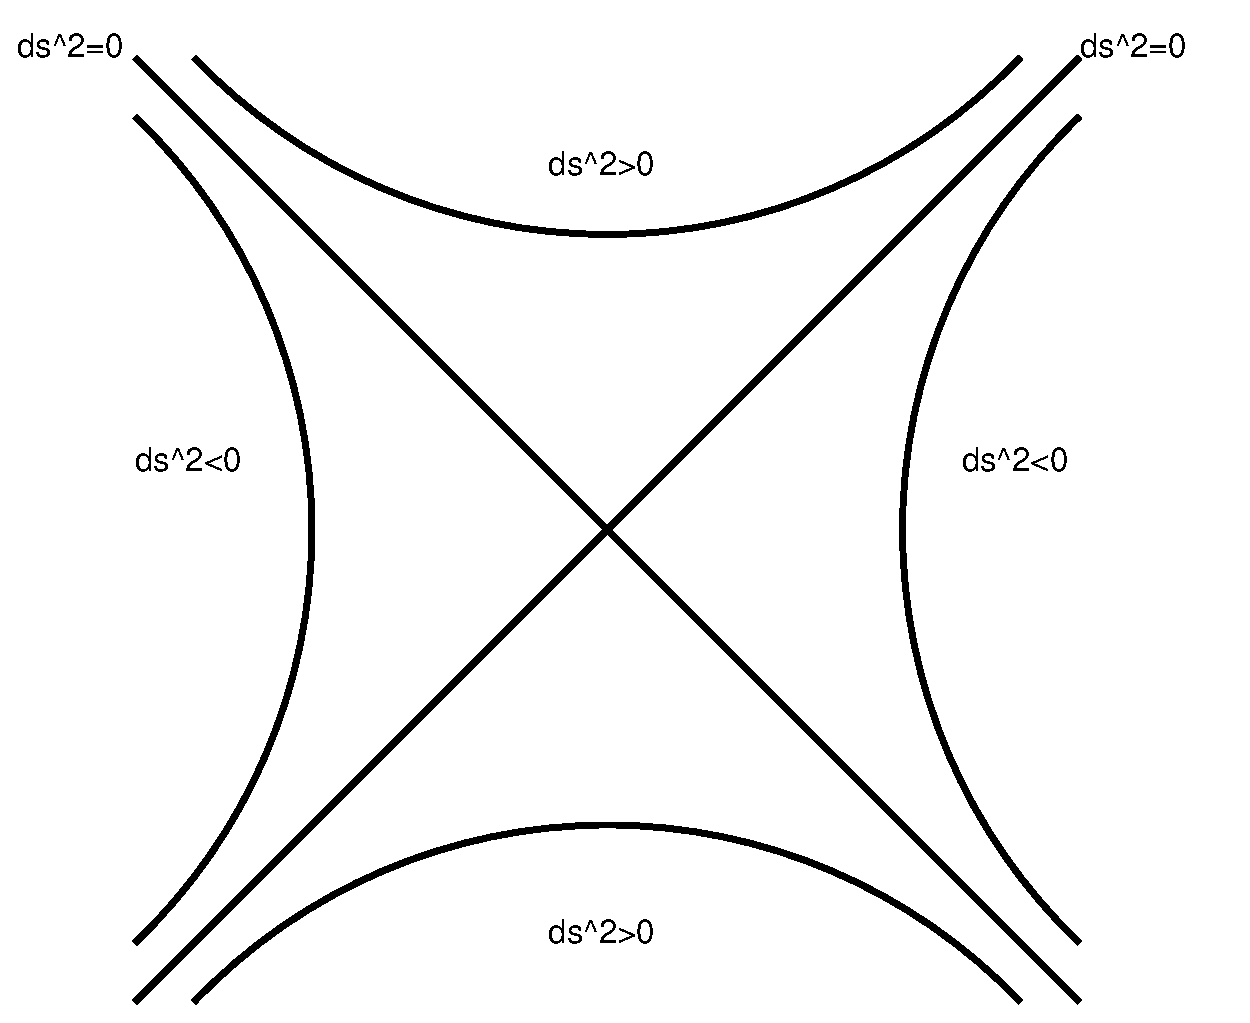
\includegraphics[width=6cm]{invariante.eps}
    \caption{Come variano le iperboli al variare della costante}
    \label{fig:iperboli}
  \end{center}
\end{figure}

% Le ascisse sono rappresentate dalle $x$, e le ordinate sono
% rappresentate da $ct$.
Le iperboli sovrastanti gli asintoti, e sottostanti ad esse, sono
quelle con cost $>\,0$, e sono le uniche che possono verificarsi
(assieme agli asintoti), in quanto solo per esse vale
$\mathsf{v}<c$. Si giunge cos\`i alla rappresentazione del cono
\index{cono di luce}di luce di un punto (nel nostro caso, quello della
figura \vref{fig:cono}).
\begin{figure}[tb]
  \begin{center}
    \psfrag{ct per x=y=z=0}{\tiny $ct$ per $x=y=z=0$} \psfrag{B}{$B$}
    \psfrag{A}{$A$} \psfrag{D}{$D$} \psfrag{E}{$E$} \psfrag{x per
      ct=0}{\tiny $x$ per $c t=0$}
    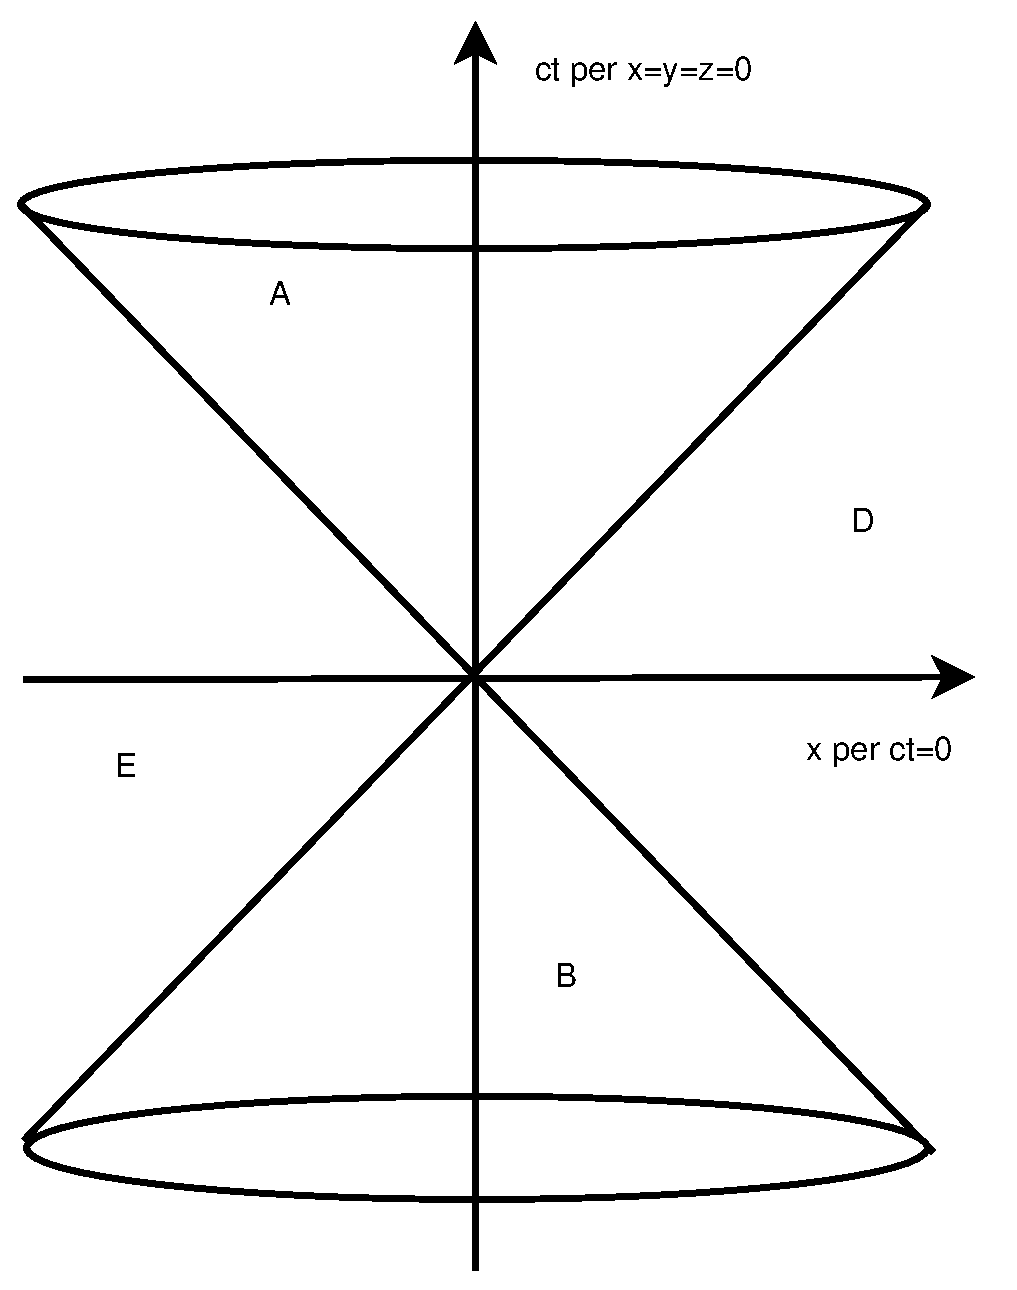
\includegraphics[width=6cm]{cono.eps}
    \caption{Cono di luce} \label{fig:cono}
  \end{center}
\end{figure}
Cos'\`e questo cono di luce? Prendiamo due raggi di luce che si
propagano da $O$, nella direzione delle $x$, con verso opposto.  Essi
descriveranno la traiettoria che, se unita, dar\`a origine al semicono
superiore. Discorso analogo per due raggi di luce che arrivano
contemporaneamente in $0$: essi descriveranno il semicono
inferiore. L'unione di questi due semiconi viene detto cono di luce
(in quanto formato da raggi di luce.). Spieghiamo pi\`u in dettaglio
il vantaggio dell'introduzione del cono di luce.  Prendiamo gli eventi
$A$ e $B$ del diagramma in figura.  L'intervallo $\de s$ sar\`a
positivo. Poich\'e tale intervallo \`e invariante sotto trasformazioni
di Lorentz, qualsiasi altro sistema di riferimento vedr\`a tale
 intervallo positivo. Tali intervalli si dicono di tipo tempo (ogni
intervallo puramente temporale \`e infatti positivo.) Gli eventi
all'esterno del cono di luce saranno invece separati da intervalli
negativi, chiamati di tipo spazio. Agli eventi sulle bisettrici degli
assi saranno invece associati intervalli di tipo luce, pari ovvero a
0. \`E facile rendersi conto che gli eventi $D$ ed $E$ possono essere
contemporanei, in qualche opportuno sistema di riferimento. Gli altri
due eventi invece no. Per questo si dice che $A$ e $B$ stanno,
rispettivamente, nel cono del futuro e nel cono del passato, in quanto
appartegono al futuro \index{futuro assoluto}e al passato assoluti
\index{passato assoluto}dell'origine degli assi (a questo punto \`e
facile capire cosa voglia dire passato e futuro assoluti). Quindi,
guardando il cono di luce di un punto, \`e subito possibile capire
molte cose sulla ``sistemazione'' temporale dell'evento, in relazione
ad altri eventi.

Si capisce anche che eventi che non appartengono al futuro o passato
assoluto, non possono essere congiunti ad $O$ tramite traiettorie.
Questo si vede geometricamente considerando la tangente di tale
traiettoria, la quale risulterebbe minore di uno, ossia $ \frac{ c \de
  t }{ \de x} < 1 \Longrightarrow v > c$, assurdo.

\begin{osservazione}
  Possiamo a questo punto notare che il fatto di poter essere
  contemporanei implica che non \`e possibile che un'informazione che
  parte da uno di questi due eventi, possa raggiungere l'altro evento,
  in nessun sistema di riferimento, proprio perch\'e dovrebbe compiere
  una traiettoria con tangente (almeno in taluni punti), minore di
  uno. Questo rende conto della finitezza della velocit\`a di
  propagazione dell'informazione.
\end{osservazione}
\section{Relativo ed assoluto}
Ci proponiamo in questa sezione di analizzare, %
%prima da un punto di
%vista geometrico, e poi da un punto di vista algebrico, 
%cosa cambia e
%cosa rimane assoluto per quello che riguarda lunghezze e tempi.
come si comportano lunghezze e tempi nella teoria della relativit\`a
speciale: il punto cruciale risulter\`a nel trovare, ancora una volta,
risultati in netto contrasto con le nostre convinzioni.

\subsection{Quello che rimane assoluto}
\label{assoluto} Nel moto di un corpo visto da diversi osservatori
rimane assoluta l'immagine del corpo nello spazio tempo (ci\`o che
viene chiamato la sua linea di universo\index{linea di universo}).
%\begin{figure}[htbp]
%  \begin{center}
%    \psfrag{ct'}{$ct'$} \psfrag{ct}{$ct$} \psfrag{x'}{$x'$}
%    \psfrag{x}{$x$} \psfrag{O}{$O$} \psfrag{R}{$R$} \psfrag{R'}{$R'$}
%    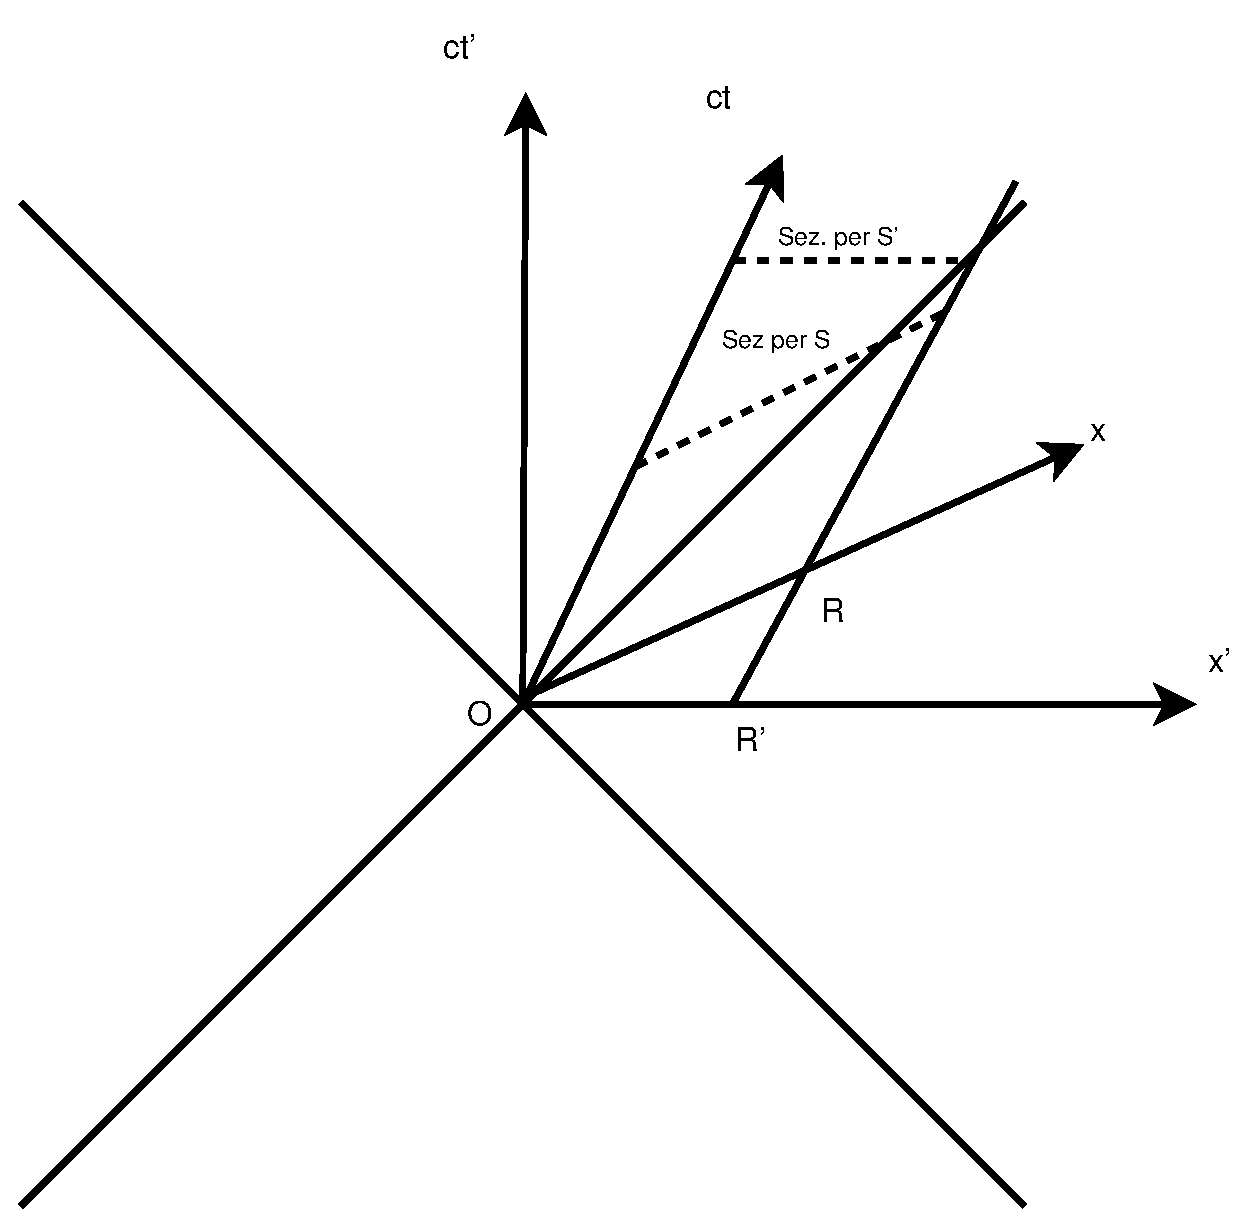
\includegraphics[height=8cm]{sezsbarra1.eps}
%    \caption{Ecco come l'immagine spazio temporale rimane la stessa
%      anche se vista da sistemi di riferimento in moto tra loro ($S$
%      ed $S'$ in questo caso)} \label{fig:Sez1}
%  \end{center}
%\end{figure}
Immaginiamo infatti di prendere un oggetto fermo nel sistema di
riferimento $S$, di assi $x$ e $ct$. Sia il corpo lungo un'unit\`a
(ragioniamo adimensionalmente, le cose non cambiano nella
sostanza). Se il corpo \`e lungo un'unit\`a, si ha:
\begin{equation}
  \mathbf{x}^2-(ct)^2\stackrel{t=0}{=}1\Longrightarrow
  \left[x\right]_{t=0}=1
\end{equation}
\begin{equation}
  \mbox{per cui } \forall t \qquad \mathbf{x}^2-(ct)^2=1
\end{equation}
e, dacch\'e questo \`e invariante, tutti gli osservatori vedono la
sbarra, \emph{nello spazio~tempo}, allo stesso modo in cui la vede
l'osservatore solidale alla sbarra, bench\'e \textbf{il modo in cui
  sia decomposta in spazio e tempo dipenda dall'osservatore.} Il fatto
che tempi e lunghezze siano ``distribuite'' in maniera diversa, si
ripercuote, portando alla contrazione di tempi e lunghezze.
\subsection{Contrazione lunghezze}
\index{contrazione delle lunghezze}
%Per analizzare la contrazione delle
%lunghezze riferiamoci alla figura \vref{fig:Sez2}; si ha:
%
%\begin{itemize} 
%\item $\overline{O'P'}=$ lunghezza 1 in $S'$\\
%\item $\overline{OP}=$ lunghezza 1 in $S$\\
%\item $\overline{O'R'}=$ lunghezza del regolo unitario a riposo in
%  $S$, misurata da $S'$\\
%\item $\overline{OR}=$ lunghezza del regolo unitario a riposo in
%      $S'$, misurata da $S$ \footnote{da qui si vede la contrazione
%        delle lunghezze: $\overline{O'R'}<\overline{O'P'}$ e
%        $\overline{OR}<\overline{OP}$}
%\end{itemize}
%
%\begin{figure}[htbp]
%  \begin{center}
%    \psfrag{ct'}{$ct'$} \psfrag{ct}{$ct$} \psfrag{x'}{$x'$}
%    \psfrag{x}{$x$} \psfrag{O}{$O$} \psfrag{R}{$R$} \psfrag{R'}{$R'$}
%    \psfrag{P}{$P$} \psfrag{P'}{$P'$}
%    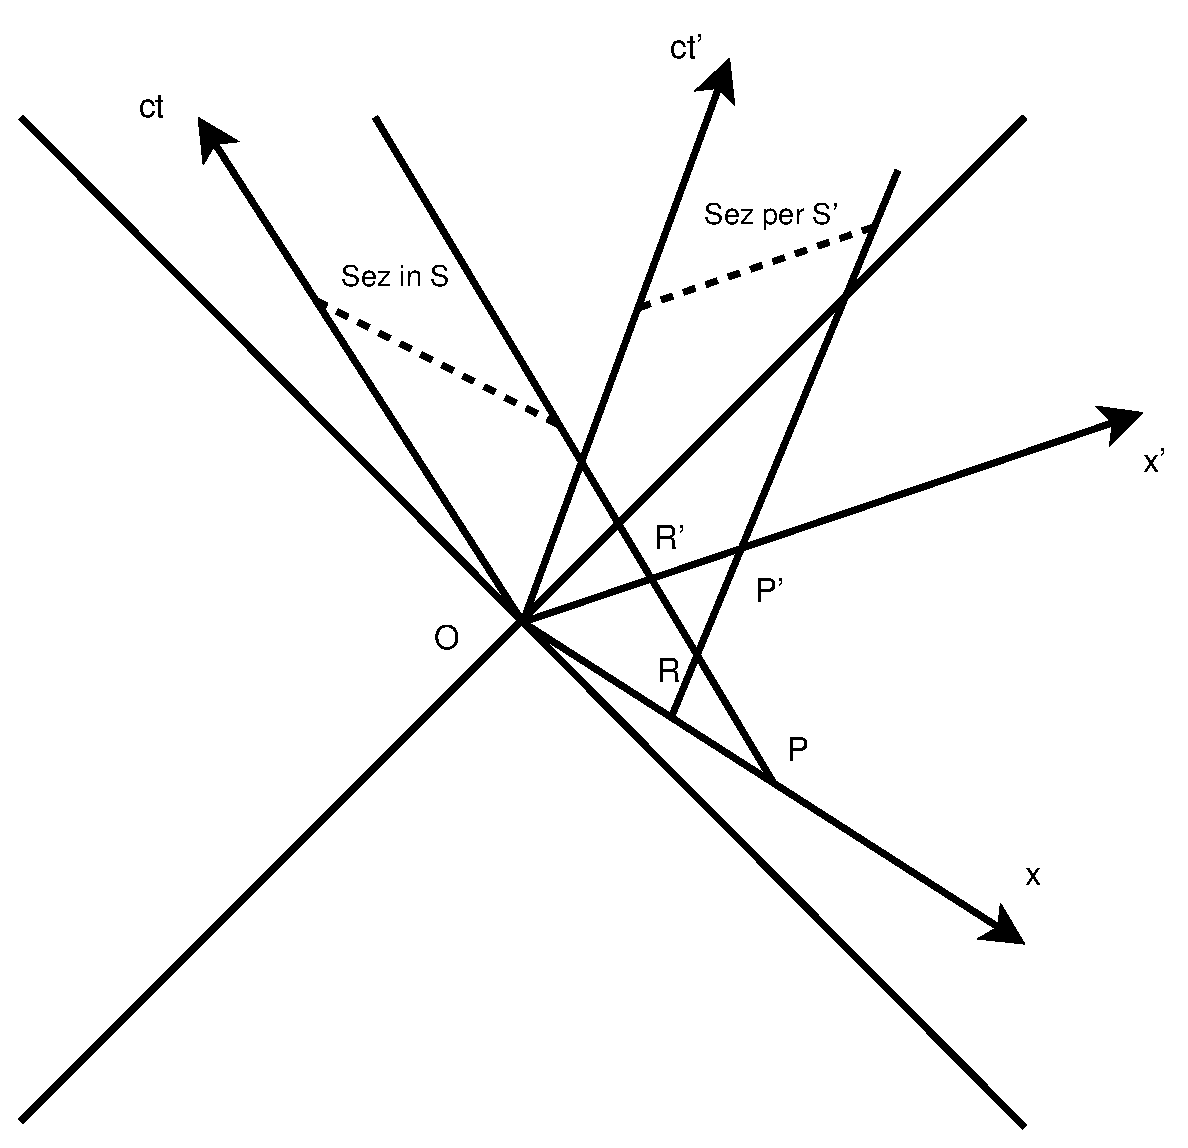
\includegraphics[height=8cm]{sezsbarra2.eps}
%    \caption{In figura si ha $OR$ ($OR'$) fotografia della sbarra
%      solidale a $S'$ ($S$) quando passa all'istante $0$ in $x$
%      ($x'$), $R'$ ($R$) \`e l'intersezione tra la sbarra in $x,c,t$
%      ($x',c',t'$) e l'asse $x'$ ($x$), $P'$ ($P$), punto dove
%      $[x']_{t'=0}=1$ ($[x]_{t=0}=1$). } \label{fig:Sez2}
%  \end{center}
%\end{figure}
%Mettiamo ora il tutto in formule, tramite le trasformazioni di Lorentz
%(\ref{eq:Lorentz}).
Per quel che riguarda la contrazione delle lunghezze, prendiamo la
 lunghezza del regolo unitario a riposo in $S'$, misurata da $S'$, pari
 a $\Delta x'$. Sia $\Delta x$ la lunghezza del regolo unitario a riposo
 in $S'$, misurata da $S$. Allora, tramite le trasformazioni di Lorentz (\ref{eq:Lorentz}):
\begin{displaymath}
  \Delta
  x'=x_{B}'-x_{A}'= \frac{x_{B} -
    \mathsf{v}t_{B}}{\sqrt{1-\frac{\mathsf{v}^2}{c^2}}} - \frac{x_{A}
    - \mathsf{v}t_{A}}{\sqrt{1-\frac{\mathsf{v}^2}{c^2}}}
\end{displaymath}
Se sono interessato alla misura effettuata da $S$, devo porre
$t_{A}=t_{B}$, e quindi:
\begin{displaymath}
  \Delta x=\Delta x'\cdot\sqrt{1-\frac{\mathsf{v}^2}{c^2}}<\Delta x'
\end{displaymath}
\subsection{Dilatazione dei tempi}
\index{dilatazione dei tempi} %Se vogliamo andare a vedere graficamente
%la dilatazione dei tempi procediamo riferendoci alla figura
%\vref{fig:Sez3}:
%\begin{figure}[htbp]
%  \begin{center}
%    \psfrag{ct'}{$ct'$} \psfrag{ct}{$ct$} \psfrag{x'}{$x'$}
%    \psfrag{x}{$x$} \psfrag{O}{$O$} \psfrag{R}{$R$} \psfrag{R'}{$R'$}
%    \psfrag{P}{$P$} \psfrag{P'}{$P'$}
%    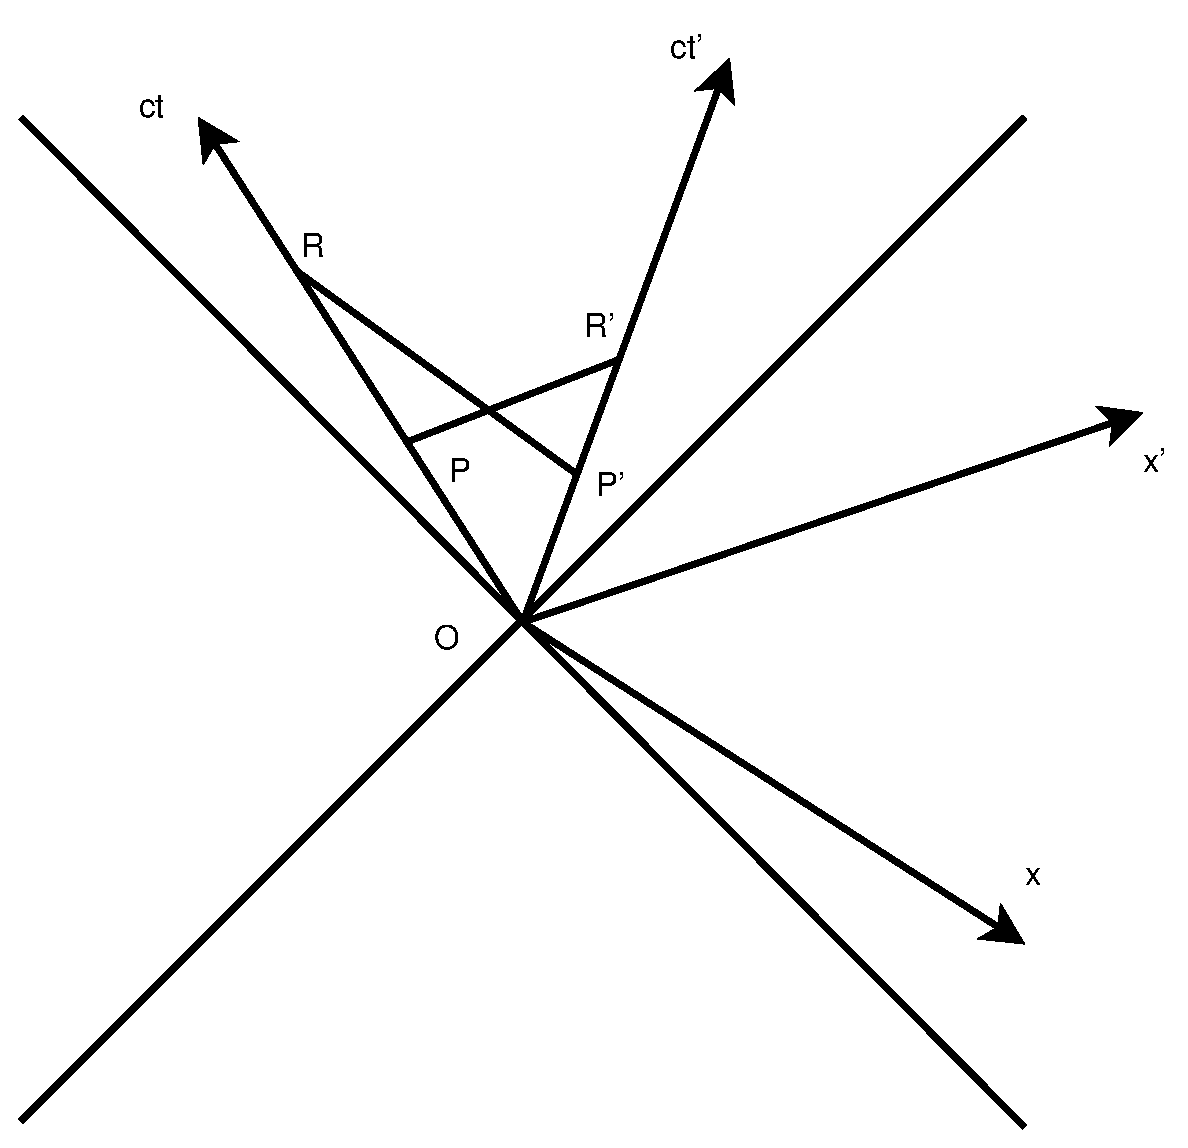
\includegraphics[height=8cm]{sezsbarra3.eps}
%    \caption{$R$ ($R'$) \`e il tempo simultaneo a $P'$ ($P$) in in $S$
%      ($S'$). $RP'$ ($R'P$) \`e segmento parallelo a $x'$
%      ($x$)}\label{fig:Sez3}
%  \end{center}
%\end{figure}
%\begin{itemize}
%\item $OP=$ tempo unitario di $S$ misurato da $S$\\
%\item $O'P'=$ tempo unitario di $S'$ misurato da $S'$\\ \item $O'R'=$
%  tempo unitario di $S$ misurato da $S'$\\
%\item $OR=$ tempo unitario di $S'$ misurato da $S$ \footnote{e da qui
%    la
%    dilatazione dei tempi: $O'R'>O'P'$ e $OR>OP$ }\\
%\end{itemize}
%Da qui si vede come i tempi ``cambiano'' a seconda del sistema di
%riferimento. Se vogliamo vedere il tutto in formule
Per vedere come i tempi sono ``influenzati'' da un cambio di sistema di
riferimento (\textbf{Attenzione: dobbiamo imporre che lo spazio sia lo
stesso se vogliamo andare a misurare i tempi}) prendiamo in
considerazione la misura del tempo di $S'$, fatta da $S$. Se voglio
misurare il tempo in $S'$, $\Delta x'$ deve essere $0$, come sopra
ricordato. Dunque:
\begin{displaymath}
\Delta t'=\frac{\Delta t-\frac{\mathsf{v}}{c^2}\Delta
  x}{\sqrt{1-\frac{\mathsf{v}^2}{c^2}}}
\end{displaymath}
\begin{displaymath}
\Delta x'=0=\frac{\Delta x-\mathsf{v}\Delta
  t}{\sqrt{1-\frac{\mathsf{v}^2}{c^2}}}
\end{displaymath}
\begin{displaymath}
\Longrightarrow \Delta x=\mathsf{v}\Delta t
\end{displaymath}
\begin{displaymath}
\Longrightarrow \Delta t'=\Delta t
\frac{1-\frac{\mathsf{v}^2}{c^2}}{\sqrt{1-\frac{\mathsf{v}^2}{c^2}}}=\Delta
t \sqrt{1-\frac{\mathsf{v}^2}{c^2}}
\end{displaymath}
\begin{displaymath}
\Longrightarrow\Delta t=\frac{\Delta
  t'}{\sqrt{1-\frac{\mathsf{v}^2}{c^2}}}>\Delta t'.
\end{displaymath}
Parlando di tempo, ci torner\`a molto utile introdurre il tempo
proprio, tramite la seguente
\begin{definizione}
  \index{tempo proprio}Il tempo proprio $\tau$ \`e il tempo misurato
  da un orologio in un sistema di riferimento in cui egli \`e fisso
  rispetto ad esso.
\end{definizione}

A noi risulter\`a comoda una definizione pi\`u ``operativa'', ovvero
si parler\`a di intervallo \index{intervallo!di tempo proprio}di tempo
proprio tra due eventi solidali al moto dell'orologio, come il tempo
necessario a quest'ultimo per misurare l'intervallo tra questi due
eventi, essendo questi fermi rispetto all'orologio; il quadrato
dell'intervallo spazio temporale avr\`a perci\`o la forma:
\begin{displaymath}
\de s^2 = c^2 \de \tau^2;
\end{displaymath}

in un altro sistema di riferimento invece
\begin{displaymath}
\de s^2 = c^2 \de t'^2 - \de \bef{x}^2=c^2 \de t'^2
(1-\frac{\bef{v^2}}{c^2}),
\end{displaymath}

il che implica $\de \tau = \de t' / \gamma$ e
\begin{displaymath}
\Delta \tau = \int_A^B \sqrt{1-\frac{\bef{v^2}}{c^2}} \de t'.
\end{displaymath}

\section{Considerazioni}
\begin{esempio}[Paradosso dei gemelli]
  A conferma di questo citiamo il famoso paradosso dei gemelli: uno
  dei due sale su un razzo con velocit\`a prossima alla velocit\`a
  della luce, l'altro rimane sulla terra. Quando quello che era sul
  razzo torna indietro risulta pi\`u giovane. Perch\'e? Considerando
  il diagramma spazio~tempo, ci accorgiamo che il sistema razzo ,
  quando esso torna verso la terra, cessa per un momento di essere
  inerziale (e se deve passare da velocit\`a prossime a~$c$ in una
  direzione, a velocit\`a prossime a~$c$ nell'altra direzione, dovr\`a
  accelerare di molto), quindi non possiamo utilizzare le
  trasformazioni della relativit\`a ristretta. Tuttavia, detto $\Delta
  \tau$ il tempo proprio del razzo, possiamo prendere:
  \begin{equation}
    \Delta \tau=(\Delta t)_{\rem{T}}\sqrt{1-\frac{\mathsf{v}^2}{c^2}}
    \label{eq:ingenua}
  \end{equation}
  Assumendo che la (\ref{eq:ingenua}) sia vera per intervalli
  infinitesimi, possiamo scrivere:
  \begin{equation}
    \de \tau=(\de
    t')_{\rem{T}}\sqrt{1-\frac{\mathsf{v}^2}{c^2}}\label{eq:ingenuabis}
  \end{equation}
  e questa \`e corretta se $\mathsf{v}$ varia nel tempo. Ora, anche se
  un punto $P'$ non \`e in moto uniforme rispetto al sistema $S$,
  possiamo considerare istante per istante (istanti $t$, non $t'$), il
  sistema di riferimento inerziale $S'(t)$, la cui velocit\`a coincide
  con quella di $P'$ all'istante $t$. Se ora consideriamo che il
  razzo, tornando indietro, passi da velocit\`a $\rem{\mathbf{v}}$ a
  velocit\`a $\rem{\mathbf{-v}}$ istantaneamente, si ha (poich\'e
  $\rem{v}$ \`e al quadrato nella formula):
  \begin{displaymath}
    t_{2}'-t_{1}'=(t_{2}-t_{1})\sqrt{1-\frac{\mathsf{v}^2}{c^2}}\:.
  \end{displaymath}

Questo risultato si rivela corretto, ma ci chiediamo: se siamo passati
istantaneamente da velocit\`a $\rem{\mathbf{v}}$ a velocit\`a
$\rem{\mathbf{-v}}$, perch\`e il gemello non vede le cose
simmetricamente rispetto al gemello sulla terra? Ovvero perch\'e egli
non vede che il gemello sulla terra \`e invecchiato della stessa
quantit\`a di quanto sia invecchiato lui? Il motivo sta nel fatto che
egli non pu\`o fare questo ragionamento (o meglio, pu\`o farlo, ma si
sbaglierebbe) poich\`e nell'inversione di velocit\`a lui cambia
sistema di riferimento, e quindi non \`e possibile applicare le
trasformazioni da noi trovate, in quanto esse valgono solo se non
cambiamo sistema di riferimento in itinere. Il gemello della terra
invece pu\`o sempre usarle, in quanto non cambia mai il proprio
sistema di riferimento.
\end{esempio}
\begin{esempio}[Decadimento $\Pi^{0}$]
  La prova sperimentale della teoria sopra esposta viene dagli
  acceleratori di particelle. Consideriamo ad esempio la particella
  neutra $\Pi^{{0}}$ (pione); quest'ultima nel suo sistema di
  riferimento (solidale alla particella) ha un tempo di vita medio
  $\tau=2\cdot 10^{-8}$s; cio\`e dopo un tempo $\tau$ il pione decade
  e si ha l'emissione di raggi gamma. $\Pi^{0}$ raggiunge una
  velocit\`a $v$ tale che $\beta \equiv \frac{v}{c}=0.99995$; quindi:
  \begin{displaymath}
    \tau'=\frac{\tau}{\sqrt{1-\beta^{2}}}=\tau \gamma \quad
    \textrm{dove}\;\frac{1}{\sqrt{1-\beta^{2}}}\equiv\gamma
  \end{displaymath}
  Si ha che $\gamma\simeq100$. Di conseguenza il tempo medio di vita
  che noi osserviamo \`e circa 100 volte superiore. Calcoliamo ora la
  distanza percorsa nell'acceleratore\index{acceleratore} da
  $\Pi^{0}$; essa sar\`a $L=v\tau\gamma\simeq600$m, mentre, non
  considerando gli effetti relativistici otteniamo $L=v\tau \simeq6$ m
  (fare bene attenzione per\`o: il $\Pi^{0}$ nel sistema di
  riferimento laboratorio decade dopo $600\,$m, ma nel suo sistema di
  riferimento vede lo spazio contratto, e quindi uguale a $ 600 \,
  \rem{ m } / \gamma = 6 \, \rem{ m }$); la differenza fra i due
  percorsi \`e bene osservabile. Aumentando la velocit\`a del pione se
  ne pu\`o aumentare il tempo di vita medio; in generale in questo
  modo sono possibili esperimenti anche su particelle che da ferme
  decadrebbero istantaneamente.
\end{esempio}
\section{Composizione delle velocit\`a}
\index{composizione delle velocit\`a}Consideriamo
$S^{\prime}$($x^{\prime}$,$t^{\prime}$) in moto rispetto ad
$S$($x$,$t$) con velocit\`a $v$ lungo $x$. Avremo quindi che:
\begin{displaymath}
  v^{\prime}_{x}=\frac{\de x^{\prime}}{\de t^{\prime}}=\frac{\de
    x-v\de
    t}{\sqrt{1-\frac{v^{2}}{c^{2}}}}\frac{\sqrt{1-\frac{v^{2}}{c^{2}}}}{\de
    t-\frac{v}{c^{2}}\de x}=\frac{\frac{\de x}{\de
      t}-v}{1-\frac{v}{c^{2}}\frac{\de x}{\de
      t}}=\frac{v_{x}-v}{1-\frac{v}{c^{2}}v_{x}}
\end{displaymath}
\begin{displaymath}
  v^{\prime}_{y}=\frac{\de y^{\prime}}{\de t^{\prime}}=\frac{\de
    y}{\de t-\frac{v}{c^{2}} \, \de
    x}\sq=\frac{v_{y}}{1-\frac{v}{c^{2}}v_{x}}\sq
\end{displaymath}
\begin{displaymath}
  v^{\prime}_{z}=\frac{v_{z}}{1-\frac{v}{c^{2}}v_{x}}\sq
\end{displaymath}
\begin{osservazione}
  Sfruttando le trasformazioni di Lorentz abbiamo ricavato le leggi di
  composizione delle velocit\`a; dobbiamo per\`o ancora verificare
  che:
  \begin{enumerate}
  \item se $v\ll c$ cio\`e $\frac{v}{c}\ll 1$ si ritorni ad avere la
    legge della composizione delle velocit\`a classica; tuttavia si
    verifica subito che:
    \begin{displaymath}
      v^{\prime}_{x}\simeq v_{x}-v\quad\textrm{quando}\;\frac{v}{c}\ll 1
    \end{displaymath}
    \begin{displaymath}
      v^{\prime}_{y}\simeq v_{y}
    \end{displaymath}
    \begin{displaymath}
      v^{\prime}_{z}\simeq v_{z}
    \end{displaymath}
  \item se $|v|=c$ ( dove $|v|=\sqrt{v_{x}^{2}+v_{y}^{2}+v_{z}^{2}}$ )
    allora anche $|v^{\prime}|=c$, dato che la velocit\`a della luce
    nel vuoto \`e la stessa per tutti i sistemi di riferimento
    inerziali. Nel caso in cui $v_{x}=c$, $v_{y}=0$, $v_{z}=0$ cio\`e
    che la luce si muova parallelamente a $v$ lungo $x$ si ha che:
    \begin{displaymath}
      v_{x}^{\prime} = 
      \frac{v_{x}-v}{1-\frac{v}{c^{2}}v_{x}}=\frac{c-v}{1-\frac{v}{c}}=c
    \end{displaymath}
    \begin{displaymath}
      v_{y}^{\prime}=0
    \end{displaymath}
    \begin{displaymath}
      v_{z}^{\prime}=0
    \end{displaymath}
    Un'altra possibilit\`a \`e il caso in cui la luce si muova
    perpendicolarmente a $v$ cio\`e: $v_{y}=c$ e $v_{x}=v_{z}=0$. Si
    ottiene:
    \begin{displaymath}
      v_{x}^{\prime}=\frac{v_{x}-v}{1-\frac{v}{c^{2}}v_{x}}=-v
    \end{displaymath}
    \begin{displaymath}
      v_{y}^{\prime}=\frac{v_{y}\sq}{1-\frac{v}{c^{2}}v_{x}}=c\sq
    \end{displaymath}
    \begin{displaymath}
      v_{z}^{\prime}=0
    \end{displaymath}
    Allora:
    \begin{displaymath}
      | v^{\prime}|=\sqrt{v^{2}+c^{2}(1-\frac{v^{2}}{c^{2}})}=c
    \end{displaymath}
  \end{enumerate}
\end{osservazione}
\section{Invarianza dell'intervallo spazio-temporale}
Cerchiamo in questa sezione di dare alcune nozioni sulle
trasformazioni che lasciano invariato l'intervallo
spazio-temporale. \`E una generalizzazione della struttura vettoriale
e dell'invarianza sotto rotazioni e traslazioni della meccanica
classica. Diamo ora una definizione importante, ed enunciamo e
dimostriamo in seguito un fondamentale teorema.
\begin{definizione}[Intervallo spazio-temporale]
  \index{intervallo!spazio-temporale} Detti $x^0 = t$, $x^1=x$,
  $x^2=y$, $x^3 =z $, definiamo la grandezza
  $s_{\rem{\scriptscriptstyle AB}}$ tale che:
  \begin{displaymath}
    s_{\rem{\scriptscriptstyle AB}}^2 = {(x_{\rem{\scriptscriptstyle
          A}}^0 - x_{\rem{\scriptscriptstyle B}}^0)}^2 -
    {(x_{\rem{\scriptscriptstyle A}}^1 - x_{\rem{\scriptscriptstyle
          B}}^1)}^2 - {(x_{\rem{\scriptscriptstyle A}}^2 -
      x_{\rem{\scriptscriptstyle B}}^2)}^2 -
    {(x_{\rem{\scriptscriptstyle A}}^3 - x_{\rem{\scriptscriptstyle
          B}}^3)}^2
  \end{displaymath}
  Chiaramente se $A$ e $B$ sono lungo una traiettoria di un raggio di
  luce, $s_{\rem{\scriptscriptstyle AB}} = 0$, mentre se $A$ e $B$
  sono lungo una traiettoria di una particella massiva, si ha $|
  \mathbf{ \rem{ v } } | < c \Longrightarrow
  s_{\rem{\scriptscriptstyle AB}} > 0$.
\end{definizione}
\begin{teorema}
  \index{teorema!dell'invarianza dell'intervallo} L'intervallo
  spazio-temporale tra due eventi \`e un invariante per trasformazioni
  tra sistemi di riferimento inerziali.
\end{teorema}
\begin{dimostrazione}Dimostriamo il tutto per intervalli infinitesimi,
  e poi estendiamo il nostro ragionamento a intervalli finiti; sia
  dunque $x_{\rem{\scriptscriptstyle B}}^{\mu} =
  x_{\rem{\scriptscriptstyle A}}^{\mu} + \de x^{ \mu }$\footnote{La
    lettera greca $\mu$ \`e un indice, che pu\`o assumere i valori da
    0 a 3.}, nel sistema di riferimento inerziale $S$; dobbiamo
  mostrare che:
  \begin{displaymath}
    \de s^2 = {(\de x^0)}^2 - {(\de x^1)}^2 - {(\de x^2)}^2 - {(\de
      x^3)}^2
  \end{displaymath}
  \`e invariante\footnote{Il modo in cui $\de s^2$ \`e stato scritto
    \`e impreciso: per i successivi sviluppi che faremo, sarebbe pi\`u
    opportuno scrivere $\de s^2 = \de x^0 \otimes \de x^0 - \de x^1
    \otimes \de x^1 - \de x^2 \otimes \de x^2 - \de x^3 \otimes \de
    x^3$, ma consci del fatto che solo gli studenti che hanno seguito
    il corso di Analisi delle Variet\`a Differenziali possono
    apprezzarlo, proseguiremo ignorando la nostra
    imprecisione.}. Prendiamo in considerazione un altro sistema di
  riferimento, sia esso $S'$; per passare da un sistema di coordinate
  all'altro si usi la funzione:
  \begin{displaymath}
    {x'}^{\mu} = f^{ \mu }( x )
  \end{displaymath}
  dove $f$ \`e una trasformazione che dipende da $\left( x^0 , x^1 ,
    x^2 , x^3 \right)$. Possiamo allora scrivere:
  \begin{equation}
    \de {x'}^{ \mu } = \sum_{\nu =0 }^{ 3 } \frac{ \partial f^{ \mu }(
      x ) }{ \partial x^{\nu} } \de x^{\nu} \label{eq:differenziale}
  \end{equation}
  La condizione di omogeneit\`a implica che $ \frac{ \partial f^{ \mu
    }( x ) }{ \partial x^{\nu} } $ sia costante, in quanto
  l'intervallo $\de {x'}^{ \mu}$ non pu\`o dipendere dal punto in cui
  mi trovo, per l'omogeneit\`a dello spazio. Pongo ora:
  \begin{displaymath}
    \frac{\partial f^{ \mu }( x ) }{ \partial x^{\nu} } := \la^{ \mu} {}_{ \nu }.
  \end{displaymath}
  Integrando la (\ref{eq:differenziale}), ottengo:
  \begin{displaymath}
    {x'}^{ \mu} = \sum_{ \nu = 0}^{ 3 } \la^{ \mu } {}_{ \nu } x^{\nu}
    + a^{ \nu },
  \end{displaymath}
  con $ a $ costante. Posso dunque scrivere:
  \begin{displaymath}
    \de {s'}^{ 2 } = {(\de {x'}^{ 0 })}^2 - {( \de {\mathbf{ x }}'
      )}^2 = \sum_{ \mu,\nu = 0}^{ 3 } \left[ \la^0 {}_{\mu} \la^0
      {}_{\nu} - \sum_{i = 1}^{ 3 } \la^i {}_{\mu} \la^i {}_{\nu}
    \right] \de x^{ \mu } \de x^{ \nu }.
  \end{displaymath}
  Definisco ora:
  \begin{displaymath}
    g_{ \mu \nu } := \la^0 {}_{\mu} \la^0 {}_{\nu} -
    \sum_{i = 1}^{ 3 } \la^i {}_{\mu} \la^i {}_{\nu} \quad
    \mbox{\scriptsize (Osserviamo che \`e simmetrico)}
  \end{displaymath}
  Allora si ha:
  \begin{displaymath}
    \de {s'}^{ 2 }= \sum_{ \mu,\nu = 0 }^{3} g_{\mu \nu} \de x^{\mu}
    \de x^{\nu}.
  \end{displaymath}
  Considero ora un raggio di luce che si propaga in $S$ lungo $x$, il
  che implica $ \de y = \de z = 0 $. Allora:
  \begin{equation}
    0 \stackrel{\rem{\scriptscriptstyle raggio \;di\; luce}}{=} (\de
    {s'})^2 = g_{00} (\de x^0)^2 + 2 g_{01} \de x^1 \de x^0 + g_{11}
    (\de x^1)^2 
    \label{eq:gmunu}
  \end{equation}
  \begin{displaymath}
    g_{01}=g_{10} \;\;\mbox{\scriptsize poich\'e simmetrico;}
  \end{displaymath}
  poi:
  \begin{displaymath}
    {\de s}^2 = {(\de x^0)}^2 - {(\de x^1)}^2 = 0 \Longrightarrow \de
    x^0 = \de x^1.
  \end{displaymath}
  Allora la (\ref{eq:gmunu}) d\`a:
  \begin{equation}
    0 = {(\de s')}^2 = (g_{00} + g_{11} + 2 g_{10}){(\de x^0)}^2;
  \end{equation}
  Se il raggio di luce si propaga nella direzione opposta, $\de x^1$
  cambia segno e dunque:
  \begin{displaymath}
    0 = {(\de s')}^2 = (g_{00} + g_{11} - 2 g_{10}){(\de x^0)}^2
  \end{displaymath}
  il che implica $ 2 g_{10} = -2 g_{10}$, e tale relazione vale se
  solo se $ g_{10} = 0$. Questo ci permette di scrivere:
  \begin{displaymath}
    0 = (g_{00} + g_{11} + 2 g_{10}) = g_{00} + g_{11} \Longrightarrow
    g_{00} = - g_{11}
  \end{displaymath}
  Per l'isotropia dello spazio, il raggio di luce potevo sceglierlo
  propagantesi anche lungo $y$ o lungo $z$, il che permette di
  concludere:
  \begin{displaymath}
    - g_{00} = g_{11} = g_{22} = g_{33}
  \end{displaymath}
  \begin{displaymath}
    g_{01} = g_{02} = g_{03} = g_{10} = g_{20} =g_{30} = 0
  \end{displaymath}

  Considero adesso un raggio di luce generico:
  \begin{displaymath}
    0 = {(\de s')}^2 = g_{00}{(\de x^0)}^2 + g_{11}{(\de x^1)}^2 +
    g_{22}{(\de x^2)}^2 + g_{33}{(\de x^3)}^2 +
    \sum_{\stackrel{i,j=1}{i\neq j}}^{3} g_{ij} \de x^j \de x^i =
  \end{displaymath}
  \begin{displaymath}
    g_{00}{(\de s)}^2 + \sum_{\stackrel{i,j=1}{i\neq j}}^{3} g_{ij}
    \de x^j \de x^i = 0 + \sum_{\stackrel{i,j=1}{i\neq j}}^{3} g_{ij}
    \de x^j \de x^i \Longrightarrow g_{ij} = 0 \mbox{ se } i \neq j
  \end{displaymath}
  Questo comporta:
  \begin{equation} {(\de s')}^2 = g_{00} {(\de
      s)}^2; 
    \label{eq:essecongi}
  \end{equation}
  domandiamoci a questo punto quanto possa valere $g_{00}$. Tale
  oggetto non pu\`o dipendere da $x$, per l'omogeneit\`a; potrebbe poi
  dipendere da $|\mathbf{v}|$, ma non da $\mathbf{v}$, per l'isotropia
  $\Longrightarrow g_{00} = g_{00}(|\mathbf{v}|)$; se scambio il ruolo
  di $S$ e di $S'$, avremo che l'unica cosa che cambia \`e
  $\mathbf{v}$ in $-\mathbf{v}$; allora:
\begin{displaymath}
\de s^2 = g_{00} (|-\mathbf{v}|)\de {s'}^2 = g_{00} (|\mathbf{v}|)\de
{s'}^2 \stackrel{(\ref{eq:essecongi})}{=} g_{00}^2 (|\mathbf{v}|)\de
{s}^2 
\end{displaymath}
\begin{displaymath}
\Longrightarrow 1 = g_{00}^2 \Longrightarrow g_{00} = \pm 1; \mbox{ se
} \mathbf{v} = 0, g_{00} = 1,
\end{displaymath}
allora $g_{00}$ \`e sempre 1, dunque $\de s^2 = \de {s'}^2$ e
\begin{displaymath}
  g_{\mu \nu}=\left(
    \begin{array}{rrrr}
      1&0&0&0\\0&-1&0&0\\0&0&-1&0\\0&0&0&-1\\
    \end{array}
  \right)
\end{displaymath}
\end{dimostrazione}

%#!simpdftex latex relativita.tex
\chapter{Formulazione geometrica}
\minitoc La formulazione geometrica della relativit\`a, presentata per
la prima volta da Minkowski, permette di trattare la relativit\`a
ristretta in maniera matematica, e dunque precisa. Questo pu\`o essere
piacevole, o causare sofferenza, a seconda delle inclinazioni
individuali\footnote{Qualche studente di fisica potrebbe rimembrare che
tali furono le parole usate dal professor Francesco Fass\`o
nell'introdurre il suo corso di Istituzioni di Fisica Matematica.}.
\section{Gruppi}
Per procedere con la nostra trattazione dobbiamo innanzi tutto
dare la definizione di gruppo, forse gi\`a nota al lettore dal corso
di metodi.

\setcounter{teorema}{-1}

\begin{definizione}
Un gruppo $\mt{G}$ rispetto all'operazione binaria $\varepsilon$ \`e un
insieme che gode delle propriet\`a seguenti:
\begin{enumerate}
\item combinando due elementi di $\mt{G}$ tramite $\varepsilon$, ottengo
      un elemento che appartiene ancora a $\mt{G}$;
\item presi tre elementi qualsiasi di $\mt{G}$, siano essi $g,h$ e $k$,
      si ha che vale la seguente uguaglianza:
\begin{equation}
 g\varepsilon(h\varepsilon k) = (g \varepsilon h) \varepsilon k;
\end{equation}
\item esiste un elemento $e$, appartenente a $\mt{G}$, detto
      \enf{elemento neutro}, tale che, $\forall\,g\in\mt{G}$
\begin{equation}
 e \varepsilon g = g \varepsilon e = g
\end{equation}

\item $\forall\,g\in\mt{G}$ esiste l'\enf{elemento simmetrico}
      $\tilde{g}$ tale che
      \begin{equation}
      g \varepsilon \tilde{g} = \tilde{g} \varepsilon g = e
      \end{equation}
\end{enumerate}
\end{definizione}
\subsection{Notazioni}
Siamo gi\`a entrati in contatto con la notazione con indici, e,
assieme ad essa, con $x^{\mu},g_{\mu\nu}$ e $\la^{\mu}{}_{\nu}$.
Ora definiamo il modo con cui indichiamo trasposta e inversa di $\la$
e inversa di $g_{\mu\nu}$, e nella notazione con indici, e nella
notazione matriciale, che potr\`a, talvolta, tornarci utile.

\begin{table}[htbp]
\begin{center}
\begin{tabular}{ccl}
Notazione con indici &$\longrightarrow$& Notazione Matriciale \\
$x^{\mu}$ &$\longrightarrow$& x \\
$\Lambda^{\mu}{}_{\nu}$ &$\longrightarrow$& $\Lambda $\\
$\Lambda_{\mu}{}^{\nu}$ &$\longrightarrow$& $\widetilde{\Lambda}$\\
$\widehat{\la}^{\nu}{}_{\mu}$ &$\longrightarrow$& $\la^{-1}$\\
$g_{\mu \nu}$ &$\longrightarrow$& $G$\\
$g^{\mu\nu}$ &$\longrightarrow$& $G^{-1}$
\end{tabular}
\end{center}
\label{tab:notazioni}\caption{Notazioni.}
\end{table}

Introduciamo anche la \textbf{convenzione di Einstein}\index{convenzione
di Einstein}, per la quale se in una formula vi sono due indici uguali,
uno in alto ed uno in basso, si intendono sommati; per intenderci: 
\begin{equation}
g_{\mu\nu}dx^{\mu}=\sum_{\mu=0}^{3}g_{\mu\nu}dx^{\mu}
\end{equation}
\begin{equation}
 \left(\mbox{ma \,\,} g_{\mu \nu} \de x^{\rho} + g_{\rho \mu} \de
x^{\nu} \neq \sum _{\mu \nu \rho} \left( g_{\mu \nu} \de x^{\rho} +
g_{\rho \mu} \de x^{\nu} \right)\right)
\end{equation} 
D'ora in poi si ha, inoltre, che le lettere greche varieranno da $0$ a
$3$, quelle latine da $1$ a $3$; cos\`i
\begin{equation}
 g_{\mu \nu} x^{\mu} = \sum_{\mu = 0 }^{ 3 } g_{\mu \nu}
x^{\mu} 
\end{equation} 
\begin{equation}
g_{i \nu} x^{i} = \sum_{i = 1 }^{ 3 } g_{i \nu} x^{i}.
\end{equation}
Introdotte queste notazioni, risulter\`a ovvio scrivere $\de s^2$ come
\begin{equation}
\de x^{\mu}g_{\mu\nu}\de x^{\nu};
\label{eq:interv_contr}
\end{equation}
nella nostra trattazione ci torneranno inoltre comode le siddette
coordinate covarianti, definite nel seguente modo:
\begin{equation}
x_{\mu} = g_{\mu\nu} x^{\nu},
\label{eq:def_covar}
\end{equation}
ovvero 
\begin{equation}
x_0 = x^0 
\end{equation}
\begin{equation}
x_i = - x^i.  
\end{equation}
Volendo scrivere la (\ref{eq:interv_contr}) tenendo conto di queste
nuove coordinate, otteniamo 
$$ \de s^2 = \de x_{\nu} \de x^{\nu}; $$
come gi\`a visto in tabella \vref{tab:notazioni}, avremo a che fare
anche con $g^{\mu\nu}$, definito come l'inverso di $g_{\mu\nu}$, e tale
che $g_{\mu \sigma} g^{\mu \rho} = \delta_{\sigma}{}^{\rho}$ (delta di
Kroenecker).

La nostra definizione sembrerebbe a prima vista del tutto inutile, in
quanto $g_{\mu \nu} = g^{\mu \nu}$; tuttavia ci\`o non \`e in generale
vero (lo \`e solo per lo spazio tempo piatto in coordinate cartesiane),
dunque la nostra definizione non \`e ridondante.  \newline Moltiplicando
per $g^{\mu \rho}$ ambo i membri della (\ref{eq:def_covar}) otteniamo:
\begin{equation}
 g^{\mu \rho} x_{\mu} = g_{\mu \nu} g^{\mu \rho} x^{\nu} = 
\delta_{\nu}{}^{\rho} x^{\nu}, 
\end{equation}
\begin{equation}
 x^{\rho} = g^{\mu \rho} x_{\mu}
\end{equation} 
da cui 
\begin{equation}
\de s^2 = g^{\mu
\nu}\de x_{\mu} \de x_{\nu}.
\end{equation}
\subsection{Condizione di invarianza}
Andiamo ora ad analizzare \textbf{la condizione di invarianza
dell'intervallo spazio temporale}. Si sa che:
\begin{equation}
 \de x^{\mu}g_{\mu\nu}\de x^{\nu}={\de x'}{}^{\mu}g_{\mu\nu}{\de x'}{}^{\nu};
\end{equation}
scrivendo il tutto in forma matriciale:
\begin{equation}
\widetilde{\de x}\;G\;\de x=\widetilde{\de x'}\;G\;\de x'
\label{eq:invariantematrice}
\end{equation}
Le trasformazioni che lasciano invariato l'intervallo avevano la
forma:
\begin{equation}\begin{array}{rcl}
{x'}{}^{\mu}      & = &\Lambda^{\mu}{}_{\nu}\;x^{\nu}+a^{\mu}; \\
                  & \mbox{dif\mbox{}ferenziando}& \\
{\de x'}{}^{\mu}  & = & \Lambda^{\mu}{}_{\nu}\,\de x^{\nu}. \\ 
                  & \mbox{In forma matriciale} & \\
\de x'            & = &\Lambda\, \de x; \\
                  & \mbox{trasponendo:} &\\
\widetilde{\de x'}& = &\widetilde{\de x}\widetilde{\Lambda}
\end{array}
\end{equation}
Allora la (\ref{eq:invariantematrice}) pu\`o riscriversi:
\begin{equation}
\widetilde{\de x} \; G \; \de x=\widetilde{\de x'} \; 
(\widetilde{\Lambda} \; G \; \Lambda) \; \de x'
\end{equation}
da cui si ricava $G=\tilde{\la}\;G\;\la$, o, con l'altra notazione
\begin{equation}
 g_{\mu \nu} = \la_{\mu}{}^{\rho} g_{\rho \sigma} \la^{\sigma}{}_{\nu}.
\end{equation}
\subsection{Gruppi di Poincar\'e e Lorentz}
Ricapitoliamo: le trasformazioni che lasciano l'intervallo
spazio-temporale invariato sono della forma, come gi\`a dimostrato:

%\marginpar{\footnotesize \vspace{0.1cm} Cogli
%indici:}\marginpar{\footnotesize
%${x'}^{\mu}=\Lambda^{\mu}{}_{\nu}\;x^{\nu}+a^{\nu}$}
\begin{equation}
x'=\Lambda x+a\quad\mbox{($a\in\mathbb{R}^4;\;\Lambda$ matrice
$4\times4$ a valori reali)}
\end{equation}
con $\Lambda$ tale che 
%\marginpar{\footnotesize$\Lambda_{\mu}{}^{\rho}
%\; g_{\rho\sigma} \Lambda^{\sigma}_{\nu}=g_{\mu\nu}$}
$\widetilde{\Lambda}\;G\;\Lambda=G$, affinch\'e l'intervallo sia
inviariante. 
%\marginpar{\vspace{0.5cm} \footnotesize si ricorda
%che}\marginpar{\footnotesize$\Lambda_{\mu}{}^{\rho} \;
%g_{\rho\sigma}\Lambda^{\sigma}{}_{\nu}=$} \marginpar{ \footnotesize
%$\sum^3_{\rho=0}\sum^3_{\sigma=0}\Lambda_{\mu}{}^{\rho} \;
%g_{\rho\sigma}\Lambda^{\sigma}{}{}_{\nu}=$}
%\marginpar{\footnotesize$g_{\nu\mu}\Rightarrow$ 16 equazioni} 
Queste leggi per le trasformazioni costituiscono un gruppo che ha come elementi
$\left\{\Lambda,a\right\}$. Le leggi di composizione sono:
\begin{equation}
\left\{\Lambda_{1},a_{1}\right\}\cdot\left\{\Lambda_{2},a_{2}\right\}=
\left\{\Lambda_{1}\Lambda_{2},\Lambda_{1}a_{2}+a_{1}\right\}
\label{eq:grppoinc}
\end{equation}
Infatti si ha $x'=\Lambda_{2}x+a_{2}$ e $x''=\Lambda_{1}x'+a_{1}$,
e dunque:
\begin{eqnarray*}
x''&=&\stackrel{x''\mbox{ in funzione di }
x}{\overbrace{\Lambda_{1}\Lambda_{2}x+\Lambda_{1}a_{2}+a_{1}}}\\
&=&(\Lambda_{1}\Lambda_{2})x+(\Lambda_{1}a_{1} + a_{2})
\end{eqnarray*}
Componendo la trasformazione $\Lambda_{1}$ con $\Lambda_{2}$
ottengo quindi la~(\ref{eq:grppoinc}).
Deve poi valere
$\widetilde{\Lambda_{1}\Lambda_{2}}\;G\;\Lambda_{1}\Lambda_{2}=G$.
Ma si constata subito che quanto appena scritto \`e uguale a:
\begin{equation}
 \widetilde{\Lambda_{2}} \widetilde{\Lambda_{1}} \; G \; 
 \Lambda_{1}\Lambda_{2}=\widetilde{\Lambda_{2}}\;G\;\Lambda_{2}=G
\end{equation}
Dunque, effettivamente la~(\ref{eq:grppoinc}) \`e una legge di
composizione. Si dimostra che \`e associativa e che l'elemento
neutro \`e:
\begin{equation}
 e=\{\rem{Id},0\}
\end{equation}
 e l'inverso \`e
\begin{equation}
\{\Lambda^{-1},-\Lambda^{-1}a\}
\end{equation}
\`e banale verificarlo usando la~(\ref{eq:grppoinc}). Il gruppo cos\`i
ottenuto con elementi \index{gruppo!di Poincar\'e} $\{\la,a\}$ \`e detto
\textbf{Gruppo di Poincar\'e $\mathscr{P}$.}  
\newline 
Il gruppo che si \index{gruppo!di Lorentz} ottiene ponendo
$a=0$ \`e detto \textbf{Gruppo di Lorentz} $\mathscr{L}$ e 
si osserva immediatamente che $\mt{L}$ ha quattro componenti
connesse; infatti una prima suddivisione \`e
\begin{eqnarray*}
\det G &=& -1 = \det (\widetilde{\la}\;G\;\la) 
\stackrel{\tiny\mbox{ Teorema  di Binet}}{=}
\det(\widetilde{\la})\;\det(G)\;\det(\la) \stackrel{\tiny \det
G=-1}{=}-(\det \la)^2\\ &&
\Longrightarrow
\det\la=\left\{
	 \begin{array}{ll} 
	  +1 \rightarrow \mt{L}_{+}\\
	 -1 \rightarrow \mt{L}_{-}
	 \end{array}
	\right.
\end{eqnarray*}
Per poter passare per\`o da $\det \la=1$ a $\det\la=-1$, si deve
fare un salto discontinuo, bench\'e, come detto prima, si abbia
che ogni singola componente sia connessa. Si ha poi:
\begin{eqnarray*}
1 = g_{00} & = & \la_{0}{}^{\mu} \; g_{\mu\nu}\la^{\nu}{}_{0} \quad 
\mbox{\footnotesize(ricordiamo che
$g_{00}\la^{0}{}_{0}=\la_{0}{}^{0}$)}\\
%
 & = & \stackrel{(\la_{0}{}^{0})^2}{\overbrace{\la_{0}{}^{0}\la_{0}{}^{0}}}
- \sum_{i=1}^{3}\la_{0}{}^{i}\la_{i}{}^{0}\\
\Longrightarrow (\la_{0}{}^{0})^2  & = &  1 +
\sum_{i=1}^{3}\la_{0}{}^{i}\la_{i}{}^{0}\geq1
\end{eqnarray*}
Ne segue
\begin{equation}
\la_{0}{}^{0} = \left\{
		 \begin{array}{ll} 
		  \geq +1 \rightarrow \la \in \mt{L}^{\uparrow}\\
		  \leq -1 \rightarrow \la \in \mt{L}^{\downarrow}
		 \end{array}
		\right.
\end{equation}
Si definisce allora il \textbf{Gruppo di Lorentz proprio}
\index{gruppo!di Lorentz proprio}come $\mt{L}^{\uparrow}_{+}$, cio\`e
tutte le $\la$ t.c.
\begin{eqnarray*}
\widetilde{\la}\;G\;\la&=&G\\
\det \la&=&1\\
\la_{0}{}^{0}&\geq&1
\end{eqnarray*}
e il \textbf{Gruppo di Poincar\'e proprio}, \index{gruppo!di Poincar\'e
proprio}ossia $\forall\;a \in \mathbb{R}^4$: 
\begin{equation}
 \mbox{se }\la\in\mt{L}^{\uparrow}_{+}
 \Longrightarrow \{\la,a\}\in\mt{P}^{\uparrow}_{+}
\end{equation}
\subsection{Particolarit\`a del gruppo di Lorentz proprio.}
 \index{gruppo!di Lorentz proprio} 
Ci domandiamo ora che forma hanno le
$\la \in \mt{L}^{\uparrow}_{+}$. Esse sono matrici $4\times4$, per\`o,
dacch\'e $G$ \`e simmetrica, le equazioni $\widetilde{\la}\;G\;\la$ sono
solo
\begin{equation}
\frac{1}{2}(\# \mbox{ fuori diagonale}) + (\#\mbox{
 diagonale})=\frac{1}{2}\;12+4=10: 
\end{equation}
10 equazioni indipendenti, il che implica $16-10 = 6$
parametri indipendenti.\footnote{Le dieci equazioni rappresentano dieci
vincoli al sistema}

Se abbiamo trasformazioni che agiscono solo su $x^1$, $x^2$, $x^3$ e
lasciano invariante l'intervallo spazio-temporale allora devono lasciare
invariato l'intervallo spaziale: le trasformazioni che danno questo
risultato sono le rotazioni: ci ritroviamo dunque con solo tre parametri
(infatti le rotazioni ne hanno ``presi'' altri tre). Riscriviamo le
trasformazioni di Lorentz speciali lungo $x^1$ ($\gamma$ e $\beta$
definite come sopra):
\begin{eqnarray*}
x'^1&=&(x^1-\beta\;x^0)\;\gamma\\
x'^2&=&x^2\\
x'^3&=&x^3\\
x'^0&=&(x^0-\beta\;x^1)\gamma. \end{eqnarray*}

Dunque: lungo il primo asse mi ritrovo un parametro, ma per
l'isotropia dello spazio, nulla mi vieta di poter fare le medesime
trasformazioni anche per gli altri due assi, ritrovandomi cos\`i
ad avere gli altri due parametri che mi servivano. In questo modo
posso caratterizzare il gruppo proprio di Lorentz, in quanto si \`e
trovato che \`e fatto da \emph{trasformazioni di Lorentz
lungo $x^1,\;x^2,\;x^3$, e da rotazioni \index{rotazioni}attorno i tre assi.}

La matrice che corrisponde alle trasformazioni speciali di Lorentz
lungo $x^1$ con velocit\`a $v$ \`e ($\la\in
\mt{L}_{+}^{\uparrow}$):
\begin{equation}
\la=\left(\begin{array}{cccc}
\gamma&-\beta\gamma&0&0\\-\beta\gamma&\gamma&0&0\\0&0&1&0\\0&0&0&1\\\end{array}\right)
\end{equation}
$$
\Rightarrow\det\la=1.
$$

Abbiamo perci\`o visto che i gruppi $\mt{P}$ e $\mt{L}$ si spezzano nei
sottogruppi (evito di riportare quelli di~$\mt{P}$):
$$
\mt{L}_{+}^{\uparrow} \quad \mt{L}_{-}^{\uparrow} \quad
\mt{L}_{+}^{\downarrow}\quad \mt{L}_{-}^{\downarrow}
$$
Possiamo introdurre ora degli operatori su questi gruppi:
\begin{dinglist}{172}
\item  Operatore di Parit\`a: $\mathit{P}\mathbf{x}=-\mathbf{x}$
$$
\mathit{P}=\left(\begin{array}{rrrr}
1&0&0&0\\0&-1&0&0\\0&0&-1&0\\0&0&0&-1\\\end{array}\right)
$$
\begin{center}
$\mathit{P}^0{}_0=1\Longrightarrow\mi{P}\in\mt{L}^{\uparrow}$\newline
$\det \mi{P}=-1\Longrightarrow\mi{P}\in\mt{L}^{\uparrow}_{-}$
\end{center}
\end{dinglist}
\begin{dinglist}{173}
\item Analogamente, considerando l'inversione temporale $\mi{T}$
$$
\mathit{T}=\left(\begin{array}{rrrr}
-1&0&0&0\\0&1&0&0\\0&0&1&0\\0&0&0&1\\
\end{array}\right)
$$
\begin{center}
$\mathit{T}^0{}_0=-1\Longrightarrow\mi{T}\in\mt{L}^{\downarrow}$
\newline
$\det \mi{T}=-1\Longrightarrow\mi{T}\in\mt{L}^{\downarrow}_{-}$
\end{center}
\end{dinglist}
\begin{dinglist}{174}
\item Inoltre si pu\`o prendere $\mi{P}\mi{T}$
$$
\mathit{PT}=\left(\begin{array}{rrrr}
-1&0&0&0\\0&-1&0&0\\0&0&-1&0\\0&0&0&-1\\
\end{array}\right)
$$
\begin{center}
$\mi{P}\mi{T}\in\mt{L}^{\downarrow}_{+}$
\end{center}
\end{dinglist}
\begin{osservazione}
Per ora non abbiamo utilizzato il principio di relativit\`a di Einstein,
il quale afferma che le leggi della fisica hanno la stessa forma in
tutti i sistemi di riferimento inerziali. Allora se sono in $ S' $ e
applico, ad esempio, l'operatore di parit\`a, mi ritrovo in un sistema
di riferimento $S$ nel quale devono valere le stesse leggi della fisica
del primo.  Invece nel '57 si scoperse che nel decadimento $\beta$
questo principio era violato in quanto l'operatore parit\`a non lascia
inviarianti le leggi della fisica. Si trova invece che le leggi della
fisica sono invarianti per $\mt{P}_{+}^{\uparrow}$, e quindi per
$\mt{L}_{+}^{\uparrow}$.
\end{osservazione}
\begin{osservazione}[dovuta a Minkowski] La distanza euclidea
infinitesima in $\mathbb{R}^3$ \`e\footnote{
da qui l'invarianza per rotazioni}:
\begin{equation}
 |d\mathbf{x}|^2=(dx^1)^2+(dx^2)^2+(dx^3)^2.
\end{equation}
L'intervallo spazio temporale ha invece la forma:
\begin{equation}
 ds^2=(dx^0)^2-|d\mathbf{x}|^2
\end{equation}
Se definisco\footnote{Si chiama rotazione di Wick quando la si applica
alla teoria dei campi} $x^4=ix^0$
\begin{equation}
 \Rightarrow ds^2=-[(dx^4)^2+(dx^1)^2+(dx^2)^2+(dx^3)^2]
\end{equation}
In questa maniera si trova un modo per trasformare nozioni
euclidee nello spazio tempo reale. Infatti l'invarianza di
$ds^2\;\;(x^1,x^2,x^3,x^4)$ \`e quella delle rotazioni
4-dimensionali (oppurtunamente complessificate); prendiamo la
rotazione di $x^4$ e $x^1$. Si ha:
\begin{eqnarray*}
\stackrel{\mathrm{Imm}}{\overbrace{x'^4}} & =
 &\cos\xi\;\stackrel{\mathrm{Imm}}{\overbrace{x^4}} 
+ \sin\xi\;\stackrel{\mathrm{Reale}}{\overbrace{x^1}}\\
x'^1&=&-\sin\xi\; x^4 + \cos \xi\; x^1\
\label{eq:sincos}
\end{eqnarray*}
Se $\xi\in\mathbb{C}$ $\sin\xi\in i\mathbb{R}$ e $\cos\xi\in\mathbb{R}$,
(altrimenti le uguaglianze non varrebbero). Perci\`o
$\xi=i\psi,\;\psi\in\mathbb{R}$, e in tal modo si ottiene
\begin{eqnarray*}
\cos\xi=\cos(i\psi)&=&\cosh\psi\\
\sin\xi=\sin(i\psi)&=& - i \sinh\psi
\label{eq:sinhcosh}
\end{eqnarray*}
Allora:
\begin{equation}
\left\{\begin{array}{l}
(x^1)'=\sinh\psi\;x^0 + \cosh\psi\;x^1\\
(x^0)'=\cosh\psi\;x^0 - \sinh\psi\;x^1
\end{array}\right.
\label{eq:iper}
\end{equation}
(la seconda non \`e altro che
$(x^4)'=i(x^0)'=\cosh\psi\;ix^0+\sinh\psi\;ix^1 \mbox{, divisa per } i$).  
Consideriamo ora un sistema $S'$ che si muove con velocit\`a $v$
rispetto ad $S$, con $x^1$ costantemente uguale a 0; si avr\`a: 
\begin{equation}
 (x^1)'=-vt'=-\frac{v}{c}(x^0)'\Rightarrow\frac{(x^1)'}{(x^0)'}=-\frac{v}{c}
\qquad(\ddagger) 
\end{equation}
Dalle (\ref{eq:iper}) risulta: 
\begin{equation}
 \frac{(x^1)'}{(x^0)'}=\tanh\psi\stackrel{(\ddagger)}{=}-\frac{v}{c}
\end{equation}
\begin{equation}
\Longrightarrow\left\{\begin{array}{l}
\sinh\psi=-\beta\;\gamma\\
\cosh\psi=\gamma
\end{array}\right.
\label{eq:tanh}
\end{equation}
\begin{equation}
 (\mbox{discende da } \cosh^2t-1=\sinh^2t)
\end{equation}
Riscrivendo la~(\ref{eq:sincos}) tenendo conto di~(\ref{eq:sinhcosh}) 
e~(\ref{eq:tanh}) ritroviamo la matrice di Lorentz, il che implica
che in relativit\`a, v'\`e l'invarianza per rotazioni complesse.
\end{osservazione}
\section{Calcolo vettoriale}
\subsection{Calcolo vettoriale in meccanica prerelati\-vi\-sti\-ca}
%Nel cominciare questa sezione, facciamo subito notare le
%differenze geometriche tra meccanica pre-relativistica e
%relativistica riportate in tabella \vref{tab:diff}.
%
%\begin{table}[!h]
%\begin{center}
%\begin{tabular}{ccc}
%Meccanica Pre-relativistica &$\longrightarrow$& Meccanica Relativistica \\
%Spazio 3-D &$\longrightarrow$& Spazio-tempo 4-D\\
%Invarianza per rotazioni &$\longrightarrow$& Invarianza per
%$\mt{L}^{\uparrow}_{+}$\\
%Metrica $\sum_{\alpha}(dx^{\alpha})^2$ &$\longrightarrow$&
%$ds^2=(dx^0)^2-(d\mathbf{x})^2$
%\end{tabular} \caption{}\label{tab:diff}
%\end{center}
%\end{table}
In meccanica pre-relativistica si usa il calcolo
vettorialea\index{calcolo vettoriale!euclideo} poich\'e, grazie ad esso,
le leggi della fisica sono covarianti per rotazioni o traslazioni, come
conseguenza dell'omogeneit\`a e dell'isotropia dello spazio. La legge di
trasformazione in questo caso \`e (se $x_i=(x_1,x_2,x_3)$):
\begin{equation}
 x_i'=\sum_{j=1}^3(R_{ij}x_{j}+a_j)\qquad \mbox{con} R { tale che }
\tilde{R}\cdot R=\mbox{Id}
\end{equation}
Gli oggetti tipici del calcolo vettoriale sono\footnote{L'apice $'$
indica l'oggetto in questione dopo la trasformazione}
\begin{itemize} 
 \item gli scalari: $A$ \`e uno scalare quando (rispetto alle
roto-traslazioni):
\begin{equation}
 A'=A
\end{equation}
 \item i vettori: $V$ \`e un vettore quando:
\begin{equation}
 V_{i}'=R_{ij}V_{j}
\end{equation}
\end{itemize}
Presa un'equazione $\mathbf{F}=m\mathbf{a}$ (in componenti $F_i=ma_i$),
nel nuovo sistema di riferimento $S'$ si ha:
\begin{equation}
 F_{j}'=R_{ij}F_i=R_{ij}ma_i=ma_{i}' \mbox{ con } R_{ij} a_i = a'_j:
\end{equation}
questo significa che nel nuovo sistema di riferimento, le leggi
sono le stesse.
\section{E in fisica relativistica\ldots? I tensori.}
\index{calcolo vettoriale!quadridimensionale} Tuttavia, in fisica
relativistica per compiere queste trasformazioni abbiamo bisogno di uno
spazio quadri-dimensionale, e non delle rotazioni, bens\`i delle
trasformazioni di Lorentz.  Si introduce dunque la nozione di tensore
quadridimensionale. Un \index{tensore}tensore $I_{ij}$ (in questo caso
si pu\`o pensare al momento d'inerzia) \`e un oggetto che trasforma come
il prodotto tra due vettori. Ovvero, se $I_{ij}\sim v_i v_j$,
$v\in\mathbb{R}^3$, si ha:
\begin{equation}
I=\left(\begin{array}{ccc} v_1v_1 & v_1v_2 & v_1v_3\\
v_2v_1 & v_2v_2 & v_2v_3\\
v_3v_1 & v_3v_2 & v_3v_3 \end{array}\right)
\label{eq:primotensore}
\end{equation}
Dacch\'e $I_{ij}\sim v_i v_j$, per rotazioni vive la seguente
relazione:
\begin{eqnarray*}
I_{ij}'&=&\sum_{l=1}^3 R_{il}v_l\sum_{k=1}^3R_{ik}v_k\\
&=&\sum_{l,k=1}^{3}R_{il}R_{jk}(v_{l}v_{k})
\end{eqnarray*}
$I_{ij}$ \`e a due indici, ma si possono introdurre quanti indici
si vogliono. Inoltre si pu\`o avere anche $I_{ij}\sim v_i u_j$, e
la (\ref{eq:primotensore}) cambier\`a di conseguenza; risulta
sempre chiaro che si possono avere tutti gli indici che si
vogliono, per esempio\footnote{$A$ \`e in questo caso un
tensore di rango 4, mentre $I$ era un tensore di rango 2}
$A_{ijkl}\sim v_i v_j v_k v_l$ (e di conseguenza
$A_{ijkl}'=\sum_{m,n,o,p=1}^{3}R_{im}R_{jn}R_{ko}R_{lp}A_{mnop}$).
Si ha che:
\begin{itemize}
\item $A_{ijkl}$ \`e un tensore di rango 4;
\item uno scalare \`e un tensore di rango 0;
\item un vettore \`e un tensore di rango 1.
\end{itemize}
\begin{esempio}[Tensore $\varepsilon$]
$$
\varepsilon_{ijk}=\left\{\begin{array}{l} \;\;\;1 \mbox{ se }
\left(\begin{array}{c}
i\\j\\k\\\end{array}\right)=\left(\begin{array}{c}
1\\2\\3\end{array}\right) \mbox{ o permutazioni pari}\\
\mbox{ }\\
-1 \mbox{ se } \left(\begin{array}{c} i\\j\\k\\\end{array}\right)
\mbox{ \`e una permutazione dispari di } \left(\begin{array}{c}
1\\2\\3\end{array}\right)\\
\mbox{}\\
0 \mbox{ altrimenti}
\end{array} \right.
$$
\end{esempio}
\begin{esempio}[Il simbolo di Kroenecker]\index{delta!di Kroenecker}
$\delta_{ij}$, non \`e altro che un tensore di rango~2.
\end{esempio}
\section{Il calcolo tensoriale\ldots}
Come prima accennato, in relativit\`a si usano i tensori; descriviamo
gli oggetti con cui entreremo in contatto(prendiamo, d'ora in poi, $\la
\in \mt{P}^{\uparrow}_{+}$):\footnote{Potr\`a a qualcuno apparire strano
di come vengano definiti questi oggetti; infatti non si asserisce nulla
di concreto su di essi, se non come essi trasformano sotto $la \in
\mt{P}^{\uparrow}_{+}$; tuttavia tale metodo, essendo il pi\`u astratto
possibile, ha dei vantaggi, dacch\'e permette di ``catalogare'' subito
gli oggetti con cui si viene a contatto; pi\`u avanti (sicuramente nel
capitolo dedicato all'elettromagnetismo), si familiarizzer\`a con questo
concetto in maniera pi\`u ``operativa''.}
\begin{itemize}
\item un quadriscalare $A$ \`e un oggetto che per trasformazioni
$\mt{P}^{\uparrow}_{+}$ si comporta in maniera tale da aversi:
$$A'=A;$$
\item un quadrivettore controvariante\footnote{Per capirsi
una volta per tutte, controvarianti sono gli oggetti con l'indice,
o gli indici, in alto, covarianti gli oggetti con indice in
basso, bench\'e la definizione precisa \`e data in base al modo in cui 
trasformano} $A^{\mu},\;\mu=1,2,3,4$, \`e tale che:
$$
A'^{\mu}=\la^{\mu}{}_{\nu}A^{\nu};
$$
\item un quadri-tensore covariante di rango 2, $A_{\mu\nu}$ \`e
tale che
$$A'_{\mu\nu}=\la^{\mu}{}_{\rho}\la^{\nu}{}_{\sigma}A_{\rho\sigma}.$$
\begin{esempio}
Il tensore metrico $g_{\mu\nu}$.
\end{esempio}
\begin{esempio}
In 3D possiamo prendere $\delta_{ij}$:
$$
\delta_{ij}=\left(\begin{array}{ccc} 1&0&0\\0&1&0\\0&0&1
\end{array}\right)
$$
\end{esempio}
\item un vettore covariante $A_{\mu}$ \`e tale che
$A_{\mu}=g_{\mu\nu}A^{\nu}$ ($A^0=A_0$ e $A^i=-A_i$). Tale oggetto
trasforma cos\`i:\footnote{$\widehat{\la}$ \`e l'inversa}
\begin{eqnarray*}
A'_{\mu}&=&\widehat{\la}^{\nu}{}_{\mu}A_{\nu} \quad \mbox{dove}\\
\widehat{\la}^{\nu}{}_{\mu}&=&g_{\mu\rho}\la^{\rho}{}_{\sigma}g^{\sigma\nu}
\end{eqnarray*}
Prendiamo $A'^{\nu}=\la^{\nu}{}_{\rho}A^{\rho}$. Si ha:
\begin{equation}
  A'_{\mu}=g_{\mu\nu}A'^{\nu} = g_{\mu\nu}\la^{\nu}{}_{\rho} 
  A^{\rho}\stackrel{\star}{=}
\end{equation}
Dacch\'e $A^{\rho}=g^{\rho\sigma}A_{\sigma}\Longrightarrow$
\begin{equation}
 \stackrel{\star}{=}\stackrel{\widehat{\la}_{\mu}{}^{\sigma}}
{\overbrace{g_{\mu\nu}\la^{\nu}{}_{\rho}g^{\rho\sigma}}}A_{\sigma}
\end{equation}
\item un quadri-tensore covariante di rango 2 \`e un oggetto $A_{\mu\nu}$
tale che:
\begin{equation}
  A_{\mu\nu}'=\widehat{\la}_{\mu}{}^{\rho}\widehat{\la}_{\nu}{}^{\sigma} 
  A_{\rho\sigma}
\end{equation}
\item un quadritensore di rango 1 covariante e di rango 1
controvariante \`e un oggetto $A_{\mu}{}^{\nu}$ che trasforma in
questo modo:
\begin{equation}
  A'_{\mu}{}^{\nu}=\widehat{\la}_{\mu}{}^{\sigma}\la^{\nu}{}_{\rho}
  A_{\sigma}{}^{\rho}
\end{equation}
\item uno pseudo-tensore \index{pseudo-tensori}\`e di prima specie se dato
$\la\in\mt{L}$, viene associato nella trasformazione il fattore
$\det\la$
\item uno pseudo-tensore \`e di seconda specie se, dato
$\la\in\mt{L}$, viene associato nella trasformazione il fattore
sgn$(\la^0{}_0)$
\item uno pseudo quadri-vettore covariante di prima specie \`e tale che, se
$\la\in\mt{L}$:
\begin{equation}
 A'_{\mu}=(\det\la)\widehat{\la}_{\mu}{}^{\nu}A_{\nu}
\end{equation}
\item uno pseudo quadri-vettore controvariante di seconda specie \`e tale che:
$$
A'^{\mu}=\mbox{sgn}\la^0{}_{0}\la^{\mu}{}_{\nu}A^{\nu}
$$
\end{itemize}
\begin{definizione}
Definiamo poi $\varepsilon_{\mu\nu\rho\sigma}$, uno pseudo-tensore di
rango 4, detto pseudo-tensore di Levi-Civita \index{Levi-Civita!simbolo
di}, tale che: 
\begin{equation}
 \varepsilon_{\mu\nu\rho\sigma} 
  = \left\{
     \begin{array}{l}
      1 \mbox{ se } \left(
		     \begin{array}{c}
		     \mu\\\nu\\\rho\\\sigma
		     \end{array}
		    \right)=
      \left(
       \begin{array}{c}
       1\\2\\3\\4
       \end{array}
      \right) 
      \mbox{ o permutazioni pari}\\ 
      \mbox{ }\\ 
      -1 \mbox{ se } 
       \left(
	\begin{array}{c}
	\mu\\\nu\\\rho\\\sigma
	\end{array}
       \right) 
       \mbox{ \`e una permutazione dispari di } 
	     \left(
	      \begin{array}{c} 
	      1\\2\\3\\4
	      \end{array}
	     \right)\\
      \mbox{}\\ 0 \mbox{ altrimenti}
     \end{array} 
    \right.
\end{equation}
Le leggi di trasformazione diventano:
\begin{equation}
 \varepsilon'^{\mu\nu\rho\sigma} = (\det \la) \la^{\mu}{}_{\alpha} 
  \la^{\nu}{}_{\beta} 
  \la^{\rho}{}_{\gamma} 
  \la^{\sigma}{}_{\delta} 
  \varepsilon^{\alpha\beta\gamma\delta}
  \stackrel{\ddagger}{=}
\end{equation}
ma
\begin{equation}
 \varepsilon^{\alpha\beta\gamma\delta} 
 \la^{\mu}{}_{\alpha} 
 \la^{\nu}{}_{\beta} 
 \la^{\rho}{}_{\gamma}
 \la^{\sigma}{}_{\delta} = 
 (\det\la)\varepsilon^{\mu\nu\rho\sigma}
 \end{equation}
e dunque:
\begin{equation}
 \stackrel{\ddagger}{=}
  (\det\la)^2 
  \varepsilon^{\mu\nu\rho\sigma}   \; \; 
  \stackrel{\tiny(\det\la)^2=1}{=} \; \;
  \varepsilon^{\mu\nu\rho\sigma}
\end{equation}
\end{definizione}
\begin{osservazione}[Analogie e differenze tra la geometria relativistica, e la geometria non relativistica]
Per una pi\`u veloce comprensione, usiamo questo utile schema
riassuntivo:
\begin{table}[htb]
\begin{center}
\begin{tabular}{ccc}
Geometria non relativistica &$\longrightarrow$& Geometria relativistica\\
$\mathbb{R}^3\Longrightarrow i=1,2,3$ & $\longrightarrow$ & 
$\mathbb{R}^4\Longrightarrow\mu=1,2,3,4$\\
$d\mathbf{x}$ invariante per rotazioni & $\longrightarrow$ & 
$\de s$ invariante per $\mt{L}$ e $\mt{P}$\\
$(d\mathbf{x})^2=\delta_{ij}dx^idx^j$ & $\longrightarrow$ & 
$(ds)^2=g_{\mu\nu}dx^{\mu}dx^{\nu} \Longrightarrow 
g_{0\mbox{}0}=-g_{i\mbox{}i}$\\
$A_i=\delta_{ij}A^{j}=A^i$ & $\longrightarrow$ & $A_i\neq A^i$
\end{tabular}
\end{center}
\end{table}
\end{osservazione}
\section{ Algebra tensoriale}
\index{calcolo tensoriale}In questa sezione ci occuperemo di meglio
definire le operazioni da compiere con gli oggetti introdotti sinora.
\subsection{ Moltiplicazioni tra vettori}
Prendiamo due vettori, $A^{\mu}$, controvariante, e $B_{\mu}$,
covariante. Vale la seguente relazione:
\begin{equation}
 A'^{\mu} B'_{\mu} = \la^{\mu}{}_{\nu}A^{\nu} 
  \widehat{\la}^{\sigma}{}_{\mu}B_{\sigma} = 
  \stackrel{\delta_{\nu}{}^{\sigma}}{\overbrace{\la^{\mu}{}_{\nu}
  \widehat{\la}^{\sigma}{}_{\mu}}} A^{\nu}B_{\mu}.
\end{equation}
Infatti, discende dalla definizione:
\begin{equation}
 \widehat{\la}^{\sigma}{}_{\mu}=g_{\mu\rho}\la^{\rho}{}_{\tau}g^{\tau\sigma};
\end{equation}
e perci\`o:
\begin{equation}
  \la^{\mu}{}_{\nu} \widehat{\la}^{\sigma}{}_{\mu} = \la^{\mu}{}_{\nu}
   g_{\mu\rho} \la^{\rho}{}_{\tau}g^{\tau\sigma} =
   (\widehat{\la}\,G\,\la)_{\nu\tau} g^{\tau\sigma} = g_{\nu\tau}
   g^{\tau\sigma} = (G\,G^{-1})_{\nu}^{\sigma} = (1)_{\nu}^{\sigma} =
   \delta_{\nu}^{\sigma}
\end{equation}
Si ha poi $A^{\mu} B_{\mu} = A^{\mu} g_{\mu\nu} B^{\nu} = A_{\nu}
B^{\nu}$: allora \`e uno scalare (per le propriet\`a degli
scalari). Ci\`o \`e del tutto analogo al prodotto scalare tra vettori
($\mathbf{A}\cdot\mathbf{B}=\sum_{i}A_i
B_i=\sum_{i,j}A_i\delta_{ij}B_j$).  Facciamo poi notare che
$A^{\mu}B_{\mu}$ ha le propriet\`a del prodotto scalare,
escluso\footnote{Dato uno spazio vettoriale
$V,\,\mathbf{A},\,\mathbf{B}\in V$, il prodotto scalare tra i due
vettori gode delle seguenti propriet\`a: \`e bilineare, definito
positivo e simmetrico} il fatto che non \`e definito positivo.
\subsection{ Contrazione degli indici}
Il processo di indici sommati viene anche detto contrazione degli
indici. Tramite tale processo si pu\`o abbassare di un grado il
rango d'un tensore;
Tramite il prodotto tra tensori, succede la stessa cosa; infatti,
se $A_{\mu\nu\rho} B^{\sigma\tau}$ \`e un tensore 3~covariante e
2~controvariante, si ha che, nel caso $\sigma=\rho$, otteniamo un
tensore 2 covariante e 1 controvariante, pi\`u precisamente
$A_{\mu\nu\rho} B^{\rho\tau}$; se invece si ha $A_{\mu} B^{\nu}$, e
$\mu = \nu$, allora, per la convenzione di Einstein,
$A_{\mu} B^{\mu} = A_0 B^0 + \ldots$, che \`e uno scalare, ovvero un
tensore di rango 0, come si dovrebbe giustamente ottenere dalla
contrazione di $A_{\mu}B^{\nu}$.
\section{ Campi tensoriali, quadrigradiente e derivate}
\begin{definizione}[Campo scalare]
\index{campo!scalare}$\varphi(x)$ \`e un \emph{campo scalare} se, sotto una
trasformazione $\{\la,a\}\in\mt{P}$, che manda $x$ in $x'=\la x +
a$, vale la relazione:
\begin{center}
$\varphi'(x')=\varphi(x)$
\end{center}
\end{definizione}
Ma come viene trasformato questo campo in funzione di $x'$? Si ha
che $x=\la^{-1}(x'-a)$: un'altra maniera di dare la
legge di trasformazione \`e dire:
\begin{center}
 $\varphi'(x')=\varphi(\la^{-1}(x'-a))$
\end{center}
Analogamente si ha:
\begin{definizione}[Campo vettoriale]
\index{campo!vettoriale}$A^{\mu}(x)$ \`e un campo vettoriale se, 
sotto $\la\in\mt{L}$,
vale la relazione:
\begin{center}
$A'^{\mu}(x')=\la^{\mu}{}_{\nu}A^{\nu}(x)$
\end{center}
\end{definizione}
Prendiamo ora in considerazione la generalizzazione di
$\mathbf{\nabla}$, ovvero il quadrigradiente.
\index{quadrigradiente}
\begin{definizione}[Quadrigradiente]
L'operatore
quadrigradiente \`e definito come:
\begin{equation}
 \partial_{\mu} \equiv \frac{\partial}{\partial x^{\mu}} = 
  \left(
   \frac{\partial}{\partial x^0}, 
   \frac{\partial}{\partial x^i}
  \right)
  =\left(
    \frac{1}{c}\frac{\partial}{\partial t},
    \mathbf{\nabla}
   \right)
\end{equation}
\end{definizione}
Dunque il quadrigradiente di un campo scalare $\varphi$ sar\`a:
\begin{equation}
 \frac{\partial \varphi}{\partial x^{\mu}} = 
  \left(
   \frac{1}{c}\frac{\partial \varphi}{\partial t},
   \mathbf{\nabla}\varphi
  \right)
\end{equation}
Ci chiediamo ora se l'oggetto $\partial_{\mu}\varphi(x)$ \`e un
vettore covariante. Verifichiamolo.
\begin{equation}
 \mathrm{d}\varphi=\frac{\partial \varphi}{\partial x^{\mu}} \, 
  \mathrm{d}x^{\mu}
\end{equation}
\`e uno scalare, quindi deve ottenersi per contrazione di un
quadrivettore covariante con uno controvariante.
\begin{definizione}
Analogamente
$\partial^{\mu}$ \`e un quadrivettore controvariante, ed \`e
definito da:
\begin{equation}
 \partial^{\mu} \equiv \frac{\partial}{\partial x_{\mu}} = 
  \left(
   \frac{\partial}{\partial x_0},
   \frac{\partial}{\partial x_i}
  \right) = 
  \left(
   \frac{1}{c}\frac{\partial}{\partial t},
   -\mathbf{\nabla}
  \right)
\end{equation}
\end{definizione}


%#!simpdftex relativita.tex
\chapter{Meccanica relativistica}
\minitoc 
In questo capitolo ci interessiamo alla
generalizzazione relativistica di velocit\`a,
accelerazione\index{accelerazione!non relativistica}, impulso e
forza. Vogliamo che tutti gli oggetti con cui si entri in contatto
siano parte dello spazio di Minkowski, sicch\'e trasformino
correttamente da un sistema inerziale ad un altro, ossia
soddisfino il principio di relativit\`a\footnote{Questo vuol dire che se
in un sistema di riferimento $F = ma$, allora in un altro sistema di
riferimento, che si pu\`o ottenere mediante una trasformazione di
Lorentz, varr\`a la relazione $F' = m' a' $}. 

Questo significa che vogliamo definire delle grandezze che si comportino
in tale modo: sia $\bef{F}$ la forza in un sistema $S$, e \(\bef{p}\)
l'impulso; in un sistema $S'$ la forza sar\`a $\bef{F'}$, e l'impulso
\(\bef{p'}\); si passer\`a dagli uni agli altri con una trasformazione di
Lorentz, ossia:
\begin{displaymath}
\bef{F}' = \la \bef{F}, 
\end{displaymath}
\begin{displaymath}
 \bef{p}' = \la \bef{p}, 
\end{displaymath}
in modo che l'equazione \(\bef{F}= \de \bef{p} / \de t\) sia la medesima
per entrambi i sistemi di riferimento, in accordo con il principio di
relativit\`a. In pratica stiamo cercando delle leggi covarianti.

Inoltre, ci preme che per $\beta<<1$, si ritrovino le quantit\`a 
classiche. Non ci cureremo per\`o di dimostrarlo, lasciandolo come facile
esercizio a cura del lettore. Ci interessa poi addentrarci nella
dinamica dei processi tra particelle, cosa di cui ci occuperemo
nell'ultima parte del capitolo.
\section{ Grandezze fondamentali}
\begin{osservazione} In cinematica non relativistica si ha:
\begin{displaymath}
 \mathbf{x}(t),\quad
 \mathbf{v}(t)=\frac{\rem{d}\mathbf{x}(t)}{\rem{d}t},\quad
 \mathbf{a}(t)=\frac{\rem{d}\mathbf{v}(t)}{\rem{d}t}
\end{displaymath}
$\mathbf{x}(t)$ \`e un vettore tuttavia: come gi\`a detto noi
vogliamo un quadrivettore. Allora:%
\footnote{\(x^\mu\), non \`e propriamente un quadrivettore, poich\'e
 sotto
una trasformazione di Poincar\'e esso diviene
 $x'^{\mu}=\la^{\mu}{}_{\nu}x^{\nu}+a^{\nu}$, ma si ovvia 
prendendone il dif\mbox{}ferenziale, ovvero
 $\rem{d}x'^{\mu}=\la^{\mu}{}_{\nu}\rem{d}x^{\nu}$.}
\begin{equation}
 \mathbf{x}\rightarrow x^{\mu}
\end{equation}
\begin{equation}
 t\rightarrow\tau \quad\mbox{ tempo proprio.}
\end{equation}
Perch\'e vogliamo usare il tempo proprio e non il tempo? La risposta sta
 nella definizione di tempo proprio (\(\de \tau = \de s /c\)): essa
 permette allo stesso di essere indipendente dal sistema di riferimento,
 al contrario di \(t\): dunque parametrizzare i moti con il tempo
 proprio, e non con il tempo, permette di ottenere un parametro che sia
 indipendente dal sistema di riferimento, e che sia quindi covariante.

 La scelta naturale cade tuttavia sulla radice di $\de s^2=\de
x^{\nu}g_{\mu\nu}\de x^{\mu}$ (solo nel caso che non si abbia a che fare
con particelle con velocit\`a pari a $c$). Per questo il lettore abbia
la cura di mostrare la validit\`a della seguente relazione (che discende
da \(\de s^2 = \de x^{\mu}\de x_{\mu}\)):
\begin{equation}
 \D s=\D t\, \frac{c}{\gamma}
\end{equation}
che ci torner\`a molto utile in seguito. Facciamo subito notare che,
 dacch\'e $\de s^2$ \`e l'intervallo spazio temporale del moto, la $v$
 all'interno di $\gamma$ \`e la velocit\`a a cui avviene il moto.
\end{osservazione}
\begin{definizione}[La quadrivelocit\`a]
\index{quadrivelocit\`a} Possiamo a questo punto prendere l'analogo
della velocit\`a:
\begin{equation}
 \mathbf{v}(t)\rightarrow \frac{\D x^{\mu}}{\D s}=\frac{\D
x^{\mu}}{c\D t}\gamma  \mbox{\scriptsize(\`e un quadrivettore,
in quanto rapporto di un quadrivettore con uno scalare ).}
\end{equation}
Si ottiene:
\begin{equation}
 u^0=\frac{\D x^0}{\D s}=\gamma,
\end{equation}
\begin{equation}
 u^i=\frac{\D x^i}{\D s}=\frac{\gamma}{c}\frac{\D x^i}{\D t};
\end{equation}
dunque, in def\mbox{}initiva, si ha:
\begin{equation}
 u^{\mu}=\left(\gamma,\frac{\gamma}{c}\mathbf{v}\right)
\end{equation}
Notiamo poi che dalla def\mbox{}inizione segue che:
\begin{equation}
 u^{\mu}u_{\mu}=1\label{eq:uperu}
\end{equation}
\begin{equation}
 \mbox{\scriptsize(al lettore i calcoli)}
\end{equation}
\end{definizione}
\begin{definizione}[La quadriaccelerazione]
\index{quadriaccelerazione} Come prima abbiamo introdotto la
quadrivelocit\`a come la derivata temporale del vettore posizione,
ora introduciamo la quadriaccelerazione come la derivata temporale
della quadrivelocit\`a:
\begin{displaymath}
 \mathbf{a}=\frac{\D \mathbf{v}}{\D t}=\frac{\D^2 \mathbf{x}}{\D
t^2}\rightarrow w^{\mu}=\frac{\D u^{\mu}}{\D s}.
\end{displaymath}
Ricaviamone le componenti (si usa qui il fatto che $\frac{\D
\gamma}{\D t}=\frac{\gamma^3}{c^2}\mathbf{v}\cdot\mathbf{a}$,
relazione che si ottiene derivando appunto $\gamma$ rispetto al
tempo, ricordando che $\mathbf{v}=\mathbf{v}(t)$):
\begin{displaymath}
 w^0=\frac{\D u^0}{\D s}=\frac{\gamma}{c}\frac{\D \gamma}{\D
t}=\frac{\gamma^4}{c^3}\mathbf{v}\cdot\mathbf{a},
\end{displaymath}
\begin{equation}
 w^i=\frac{\D u^i}{\D s}=\frac{\gamma}{c^2} 
\frac{\D (\gamma v^i)}{\D t} 
  =
  \frac{\gamma^2}{c^2}a^i + 
  \frac{\gamma^4}{c^4}(\mathbf{v}\cdot\mathbf{a})v^i; 
\end{equation}
prendiamo ora la (\ref{eq:uperu}), e deriviamola rispetto a $s$.
Ne esce:
\begin{equation}
w\cdot u=0 \label{eq:perpendicolari}
\end{equation}
il che implica che quadri-velocit\`a e quadri-accelerazione sono tra loro
ortogonali (sempre!).
\end{definizione}
\begin{definizione}[Il quadrimpulso]
\index{quadrimpulso}Si generalizza ora l'idea di impulso:
\begin{equation}
 \mathbf{p}=m\mathbf{v}\rightarrow p^{\mu}:=mcu^{\mu}
\end{equation}
Dunque il quadrimpulso risulta:
\begin{equation}
 p^{\mu} = 
  \left(\frac{mc}{\sq},\frac{m\mathbf{v}}{\sq}\right)\label{eq:quadrimpulso}
\end{equation}
Viene ora spontaneo interrogarsi su $mc\gamma$, il primo termine
del quadrimpulso: esso infatti \`e $\frac{E}{c}$. Cosa c'\`e di
strano? Prendiamo il caso $\beta<<1$. Non \`e
dif\mbox{}f\mbox{}icile vedere che:
\begin{equation}
 cp^0=mc^2\gamma \stackrel{\beta<<1}{\simeq}mc^2+\frac{1}{2}mc^2
\frac{v^2}{c^2}=mc^2+\frac{1}{2}mv^2
\end{equation}
Ora, se $\frac{1}{2}mv^2$ \`e chiaramente l'energia cinetica, non
si ha un analogo classico per il termine~$mc^2$,
\index{energia!massa@$mc^2$}in quanto da ci\`o che s'\`e appena
scritto, risulta che un corpo in quiete, per il solo fatto di
avere massa, ha un'energia pari a~$mc^2$. Saremmo tentati di
definire l'energia come $cp^0-mc^2$, ma questo oggetto non
trasforma come un tensore, e viola il principio di relativit\`a.
Osserviamo ora che:
\begin{equation}
p^{\mu}p_{\mu}=\frac{E^2}{c^2}-\mathbf{p}\;{}^{2} =
\frac{m^2c^2}{1-v^2/c^2}-\frac{m^2v^2}{1-v^2/c^2}=m^2c^2
\label{eq:masshell}\end{equation}\index{equazione!mass shell}
Questa relazione vive anche se un corpo ha velocit\`a della luce
(e quindi massa nulla), e si scrive come $E=c|\mathbf{p}|$.
\end{definizione}
\section{ La quadriforza}
\begin{osservazione}[Particella non soggetta a forze] Se una particella \`e in
moto nello spazio di Minkowski, essa \`e soggetta alle equazioni
\begin{equation}
 \frac{\de p^{\mu}}{\de s}=0\qquad\mbox{e }p^{\mu}p_{\mu}=m^2c^2,
\end{equation}
sempre che si sia in assenza di forze. Nel caso di una particella
di massa nulla, non potendo parametrizzare con $\de s$, in quanto
esso \`e sempre pari a 0, parametrizzeremo con un parametro
scalare $\zeta$; pi\`u precisamente:
\begin{equation}
 \frac{\de^2x^{\mu}}{\de \zeta^2}=0,\quad \mbox{ con } ds=0
\end{equation}
\end{osservazione}
\begin{definizione}[La quadriforza]
\index{quadriforza} Se una particella \`e invece soggetta a forze
esterne, vive la seguente relazione:
\begin{equation} \frac{\de p^{\mu}}{\de s}=\mt{F}^{\mu}
\label{eq:covariantem}
\end{equation}
\begin{center}
\scriptsize Equazione covariante di Minkowski\index{equazione!di
Minkowski}\index{Minkowski!equazione di}
\end{center}
Nel caso si voglia trovare esplicitamente i termini di $\mt{F}$,
deriviamo rispetto a~$s$ la~(\ref{eq:quadrimpulso}), ottenendo:
\begin{equation}
 \mt{F}^{\mu}=\left(\frac{\gamma}{c^2}\frac{\de E}{\de
t},\frac{\gamma}{c}\frac{\de \mathbf{p}}{\de t}\right)
\end{equation}
Ma $\de \mathbf{p}/ \de t$ non \`e altro che la $\mathbf{F}$ della
meccanica pre-relativistica, e inoltre, dacch\'e sussiste la legge
della potenza, si ha che vive la relazione $\frac{\de E}{\de
t}=\mathbf{F}\cdot\mathbf{v}$. Questo semplif\mbox{}ica un po' le
cose, permettendo di scrivere:
\begin{equation}
\mt{F}^{\mu}=\frac{\gamma}{c}
\left(\frac{1}{c}\mathbf{F}\cdot\mathbf{v}, \mathbf{F}\right).
\end{equation}
Analogamente alla (\ref{eq:perpendicolari}) si trova:
\begin{equation}
 \mt{F}^{\mu}u_{\mu} = \mt{F}^0 - 
  \frac{\mathbf{\mt{F}}\cdot\mathbf{v}}{c}=0
\end{equation}
Da qui \`e possibile vedere che $\mt{F}^{\mu}$ non \`e
indipendente da $\mathbf{v}$, cosa che prima accadeva.
\end{definizione}
\section{ Sistemi di riferimento}
Nei fenomeni in cui si ha a che fare con particelle che
interagiscono a velocit\`a prossime a quelle della luce, si rende
indispensabile la meccanica relativistica, poich\'e essa
descrive in maniera corretta le quantit\`a in gioco.
Questo spiega il larghissimo uso che se ne fa in
fisica nucleare e sub-nucleare. In questa sezione
affronteremo decadimento di particelle e urti tra
particelle.

%\vspace{0.5cm}

Per quanto riguarda la nostra analisi di urti e decadimento,
prenderemo in considerazione due sistemi di riferimento, il
sistema di riferimento del centro di massa, $\cem$, e il sistema
di riferimento del laboratorio, $\lab$\footnote{ Per capirci: in
$\cem$ il centro di massa del sistema \`e fermo, mentre $\lab$ \`e
il sistema che non \`e propriamente quello del laboratorio, ma un
altro sistema che risulta a noi comodo per descrivere i fenomeni
che studiamo}. Facciamo un esempio per impratichirsi un po' con
questi due sistemi;

\begin{esempio} Mettiamoci in $\lab$, e consideriamo due particelle, la prima
che si muove lungo l'asse $x$ con quantit\`a di moto
$\mathbf{p}_1=p$, e la seconda, ferma, per la quale vale dunque la
relazione $\mathbf{p}_2=0$. Perci\`o la sua energia \`e (sia $c=1$
in tutti i conti che facciamo in questo esempio) $E_2=m_2$. Si ha
poi:
\begin{equation}
 p_1=(E_1,p,0,0)
\end{equation}
\begin{equation}
 p_2=(m_2,0,0,0)
\end{equation}
\begin{equation}
E_1=\sqrt{p^2+m_1^2}.\label{eq:energiaur}
\end{equation}
In $\cem$ si ha invece che la quantit\`a di moto totale \`e nulla,
e dunque:\footnote{Introduciamo ora la seguente notazione: ogni
quantit\`a contrassegnata da $\star$, verr\`a intesa come
calcolata nel centro di massa, indipendentemente dal fatto che
$\star$ \ sia posizionata in alto o in basso (ovvero
$p^{\star}=p_{\star}$), per questioni di comodit\`a.}
$$
\mathbf{p}_1^{\star}+\mathbf{p}_2^{\star}=0
$$
il che porge:
$$
|\mathbf{p}_1^{\star}|=|\mathbf{p}_2^{\star}|=p^{\star}
$$
Dunque:
$$
p_1^{\star}=(E_1^{\star},p^{\star},0,0)
$$
$$
p_2^{\star}=(E_2^{\star},-p^{\star},0,0)
$$
Per passare da $\lab$ a $\cem$ si effettua una trasformazione di
Lorentz lungo $x$. Prima di farlo introduciamo tuttavia le
quantit\`a $p_{\rem{tot}}$ e $p_{\rem{tot}}^{\star}$, cos\`i
definite:
$$
p_{\rem{tot}}=p_1+p_2=(E_1+m_2,p,0,0)
$$
$$
p_{\rem{tot}}^{\star}=p_1^{\star}+p_2^{\star}=(E_1^{\star}+E_2^{\star},0,0,0)
$$
Applicando le trasformazioni di Lorentz lungo $x$ otteniamo:
\begin{equation}
(p_{\rem{tot}}^{\star})_x=\gamma_{\rem{CM}}[(p_{\rem{tot}})_x -
\beta_{\rem{CM}}p_{\rem{tot}}^{0}] \label{eq:lorenzx}
\end{equation}
Ricordando che $c=1$, si ha che $\beta_{\rem{CM}}=\rem{v}$
($\rem{v}$ \`e la velocit\`a di $\cem$ rispetto a $\lab$), e
la~(\ref{eq:lorenzx}) porge:
$$
(p_{\rem{tot}}^{\star})_x = 0
=\gamma_{\rem{CM}}[p-\beta_{\rem{CM}}(E_1+m_2)],
$$
che a sua volta d\`a:
$$
\beta_{\rem{CM}}=\frac{p}{E_1+m_2}.
$$
Dacch\'e $p=m_1\gamma_{v_1}v_1$, usando la (\ref{eq:energiaur}),
si trova $E_1=m_1\gamma_{v_1}$, dalle quali:
$$
\beta_{\rem{CM}}=\frac{m_1\gamma_{v_1}v_1}{m_1\gamma_{v_1}+m_2}=\rem{v} 
$$
Volendo esprimere~$\beta_{\rem{CM}}$ in un'altra forma, usiamo le
trasformazioni di Lorentz lungo~$z$ per la particella~2,
ottenendo:
$$
0=\gamma_{\rem{CM}}(-p^{\star}+\beta_{\rem{CM}}E_2^{\star})
$$
Con qualche semplice passaggio si arriva a:
\begin{equation}
\beta_{\rem{CM}}=\frac{p^{\star}}{E^{\star}_2}=v_2^{\star}.
\label{eq:beta}
\end{equation}
Questo risultato era da aspettarsi, in quanto per annullare la
velocit\`a della particella ferma in~$\lab$, velocit\`a che
in~$\cem$ vale~$v_2^{\star}$, \`e necessaria una trasformazione
che abbia $\beta_{\rem{CM}}=v_2^{\star}$.
\end{esempio}
\section{ Processi tra particelle (dinamica relativistica)}
\subsection{ Decadimento}\index{decadimento}
Dopo esserci impratichiti\footnote{Si spera!} con i nuovi sistemi
di riferimento che useremo nelle nostre analisi, affrontiamo pi\`u
approfonditamente il fenomeno del decadimento. il quale consiste
nel processo che, da un particella iniziale con massa $M$,
restituisce $n$ particelle separate $m_1\ldots m_n$, come in
figura \vref{fig:decadimento}.

\setlength{\unitlength}{1mm}

\begin{figure}[htbp]
\begin{center}
\begin{picture}(80,50)
\put(0,0){\framebox(80,50)}
\put(5,25){\vector(1,0){40}}\put(25,27){$M$}\put(45,25){\vector(1,1){20}}
\put(45,25){\vector(1,-1){20}} \put(45,25){\vector(2,1){24}}
\put(50,37){$m_1$}\put(50,12){$m_n$} \put(45,25){\line(3,-2){4}}
\put(51,21){\line(3,-2){4}}\put(57,17){\line(3,-2){4}}
\put(63,13){\vector(3,-2){5}} \put(60,30){$m_2$}
\end{picture}
\end{center}
\caption{Decadimento di una generica particella con massa
$M$}\label{fig:decadimento}
\end{figure}

Ci si aspetterebbe, abbastanza intuitivamente, che
$m_1+\ldots+m_n=M$; invece ci\`o non accade, poich\'e ci\`o che si
conserva \`e il quadrimpulso \index{quadrimpulso!conservazione
del}, nel caso si sia in assenza di forze esterne. La prima
domanda che viene spontaneo chiedersi \`e, date le masse delle
particelle, quali sono le condizione affinch\'e avvenga il
decadimento. Se siamo nel sistema di riferimento del centro di
massa, vale la seguente relazione:
$$
\frac{E^{\star}}{c}=Mc=\sum_{i=1}^{n}\frac{E^{\star}_{i}}{c}.
$$
Si vede subito che:
$$
\sum_{i=1}^{n}\frac{E^{\star}_{i}}{c}\geq\sum_{i=1}^{n}m_{i}c$$
$$\Longrightarrow$$
\begin{equation}
\fbox{$\displaystyle M\geq\sum_{i=1}^{n}m_{i}$}
\label{eq:decadimento}
\end{equation}
La (\ref{eq:decadimento}) \`e dunque la condizione per avere il
decadimento della particella~$M$ in~$n$ particelle.
\subsection{ Decadimento a due corpi}
Consideriamo ora il decadimento a due corpi, ovvero $M\rightarrow
m_{1}+m_{2}$. In questo caso in $\cem$, $E_{1}^{\star}$ ed
 $E_{2}^{\star}$, sono completamente determinate. Vive la
relazione:
$$
\mathbf{p}^{\star}_{1}+\mathbf{p}^{\star}_{2}=0\Rightarrow
|\mathbf{p}^{\star}_{1}|=|\mathbf{p}^{\star}_{2}|=p^{\star}\Rightarrow
\mathbf{p}^{\star}_{1}\cdot\mathbf{p}^{\star}_{2}=-p_{\star}^2
$$
Il fatto che $|\mathbf{p}^{\star}_{1}|=|\mathbf{p}^{\star}_{2}|$
comporta che:
\begin{equation}
(p_1^{\star})^2=(E^{\star}_{1})^2-m^2_1c^2=(E^{\star}_{2})^2-m^2_2c^2=(p_2^{\star})^2
\label{eq:endec1}
\end{equation}
Per la legge di conservazione dell'energia si ha:
\begin{equation}E^{\star}_{1}+E^{\star}_{2}=Mc^2.\label{eq:nuova}\end{equation}
Dividendo membro a membro le ultime due equazioni, tramite
semplici passaggi si giunge~a:
\begin{equation}
E^{\star}_{1}-E^{\star}_{2}=\frac{m^2_1-m^2_2}{M}.
\label{eq:endec2}
\end{equation}
A questo punto una semplice manipolazione algebrica della
(\ref{eq:nuova}) e della (\ref{eq:endec2}) ci porta a:
\begin{equation}
E^{\star}_{1}=c^2\frac{M^2+m^2_1-m^2_2}{2M} \label{eq:endecfin1}
\end{equation}
\begin{equation}
E^{\star}_{2}=c^2\frac{M^2-m^2_1+m^2_2}{2M} \label{eq:endecfin2}
\end{equation}
\begin{equation}
(\frac{E^{\star}_{1}}{c} - m_1^2
c^2)=p^2_{\star}=c^2\frac{M^4+m_{1}^4+m_{2}^4-2m_{1}^2m_{2}^2-2(m_{1}^2+m_{2}^2)M^2}{4M^2}
\end{equation}
Osserviamo che nel decadimento tra particelle, l'angolo
$\vartheta^{\star}$ della figura \vref{fig:decaincm} non \`e
determinato.

\begin{figure}[htbp]
\begin{center}
\begin{picture}(80,50)
\put(0,0){\framebox(80,50)}
\put(5,25){\line(1,0){4}}\put(12,25){\line(1,0){4}}\put(20,25){\line(1,0){4}}
\put(28,25){\line(1,0){4}}\put(36,25){\line(1,0){4}}\put(44,25){\line(1,0){4}}
\put(40,25){\vector(3,1){15}}\put(40,25){\vector(-3,-1){15}}\qbezier(53,25)(54,28)(52,29)
\qbezier(44,25)(40,22)(34,23)\put(48,31){$m_1$}\put(28,17){$m_2$}
\put(57,27){$\vartheta_1=\vartheta_{\star}$}
\put(40,19){$\vartheta_2=\pi-\vartheta_{\star}$}
\put(52,25){\line(1,0){4}}\put(60,25){\line(1,0){4}}\put(68,25){\line(1,0){4}}
\end{picture}
\end{center}
\caption{Decadimento a due corpi in $\cem$}\label{fig:decaincm}
\end{figure}

Esaminiamo per\`o il decadimento nel sistema laboratorio, il quale
si muove con velocit\`a~$-\mathbf{v}$ rispetto alla particella che
decade, ovvero rispetto a $\cem$. Le cose vanno come in
f\mbox{}igura~\ref{fig:decainlab}

\begin{figure}[htbp]
\begin{center}
\begin{picture}(80,50)

\put(5,38){\vector(0,1){6}}\put(5,38){\vector(1,0){6}}
\put(9,36){\scriptsize$x$} \put(3,42){\scriptsize$y$}
\put(0,0){\framebox(80,50)}
\put(5,25){\vector(1,0){40}}\put(25,27){$M$}\put(45,25){\vector(1,1){20}}
\put(45,25){\vector(1,-1){20}}
\put(50,37){$m_1$}\put(50,12){$m_n$}\multiput(45,25)(6,0){4}{\line(1,0){4}}
\put(53,27){$\vartheta_1$}\put(53,21){$\vartheta_2$}
\qbezier(51,25)(52,27)(50,30)\qbezier(52,25)(52,23)(50,20)\end{picture}
\end{center}
\caption{Decadimento a due corpi in $\lab$}\label{fig:decainlab}
\end{figure}

Possiamo dunque usare le trasformazioni di Lorentz, usando gli
assi come in f\mbox{}igura \vref{fig:decainlab}, in particolare
con l'asse $x$ posto lungo la traiettoria della particella con
massa $M$, e $z$ orientato coerentemente. Usiamo poi $\alpha=1,2$
per indicare la particella 1, o la particella 2. Trasformiamo
dunque $p^{\mu}=(E,\mathbf{p})$ lungo l'asse $x$. In $\cem$ si ha:
$$
p_{\alpha x}^{\star}=p^{\star}\cos\vartheta_{\alpha}^{\star}
$$
$$
p_{\alpha y}^{\star}=p^{\star}\sin\vartheta_{\alpha}^{\star}
$$
Dacch\'e l'energia si trasforma come il tempo, avremo:
$$
E_{\alpha}=\gamma(E_{\alpha}^{\star}+v\,p_{\alpha
x}^{\star})=\gamma(E_{\alpha}^{\star}+v\,p_{\alpha
}^{\star}\cos\vartheta_{\alpha}^{\star}),
$$
mentre per $\mathbf{p}$:
\begin{equation}
p_{\alpha x}=(p^{\star}_{\alpha x} +
\frac{\beta}{c}E_{\alpha}^{\star})\gamma =
(p^{\star}\cos\vartheta_{\alpha}^{\star} +
\frac{\beta}{c}E_{\alpha}^{\star})\gamma \label{eq:decapx}
\end{equation}
\begin{equation}
p_{\alpha
y}=p^{\star}\sin\vartheta_{\alpha}^{\star}\label{eq:decapy}
\end{equation}
\begin{equation}
p_{\alpha z}=p_{\alpha z}^{\star}=0
\end{equation}
Questo mostra che tutte le quantit\`a in gioco, eccetto
$\vartheta^{\star}$, sono note. Come in f\mbox{}igura
\ref{fig:decaincm}, valgono le seguenti relazioni:
\begin{eqnarray*}
\vartheta^{\star}_{\alpha}&\stackrel{\alpha=1}{=}&\vartheta^{\star}\\
\vartheta^{\star}_{\alpha}&\stackrel{\alpha=2}{=}&\pi-\vartheta^{\star}
\end{eqnarray*}
Andiamo a vedere il luogo geometrico di $p_{\alpha x}$ e
$p_{\alpha y}$ al variare di $\vartheta^{\star}$. Sommiamo in
quadratura la (\ref{eq:decapx}) e la (\ref{eq:decapy}); con
semplici passaggi ne esce (per la \vref{eq:decapx}, prima si
divide per $\gamma$, poi si porta a primo membro
$\frac{\beta}{c}E^{\star}_{\alpha}$):%
\footnote{$\;\;\beta=\frac{v}{c}$}
\begin{equation}
\left(\frac{p_{\alpha
x}}{\gamma}-\frac{\beta}{c}E_{\alpha}^{\star}\right)^2+p_{\alpha
y}^2=p_{\star}^2
\end{equation}
che pu\`o essere riscritta come:
\begin{equation}
(1-\beta^2)\left(p_{\alpha
x}-\frac{\beta}{c}E_{\alpha}^{\star}\gamma\right)^2+p_{\alpha
y}^2=p_{\star}^2. \label{eq:decaellisse}
\end{equation}
La (\ref{eq:decaellisse}) \`e l'equazione di un ellisse nelle
variabili $p_x,p_y$, con centro in:
$$
\left(\frac{\beta}{c}\frac{E_{\alpha}^{\star}}{\sq}\equiv
d,0\right)
$$
e semiassi:
$$
s_x=p_{\star}\gamma\quad\mbox{ lungo }x
$$
$$
s_y=p_{\star}\quad\mbox{ lungo }y
$$
Ci\`o implica i seguenti casi:
\begin{enumerate}
\item se $d<s_x$, l'angolo $\vartheta_{\star}$ pu\`o assumere
tutti i valori, come in f\mbox{}igura \vref{fig:ellisse1}

\begin{figure}[htbp]
\begin{center}
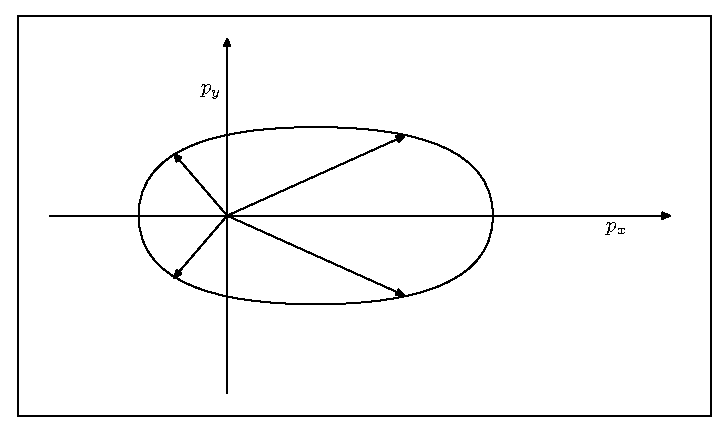
\includegraphics[height=7cm]{ellisse1.eps}
\caption{ } \label{fig:ellisse1}
\end{center}
\end{figure}

\item se $d>s_x$, l'angolo $\vartheta_{\star}$ ha un massimo,
ossia le particelle devono essere emesse in avanti, come in
f\mbox{}igura \vref{fig:ellisse2}, dove, tra l'altro, si vede
molto bene che v'\`e un angolo massimo, indicato l\`i con
$\vartheta_{\rem{max}}$, di emissione per la particella.

\begin{figure}[htbp]
\begin{center}
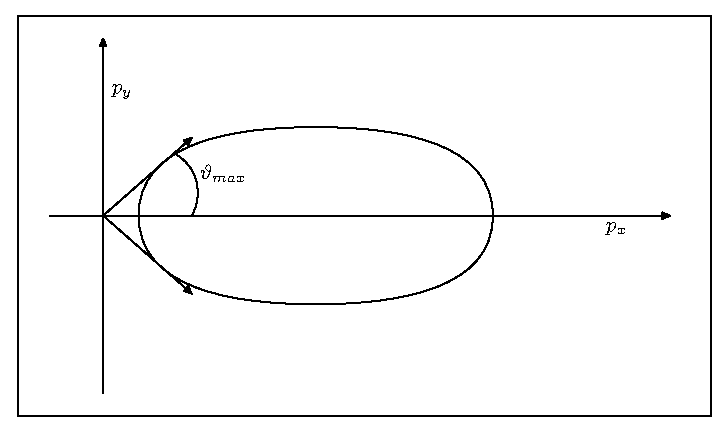
\includegraphics[height=7cm]{ellisse2.eps}
\caption{ } \label{fig:ellisse2}
\end{center}
\end{figure}
\end{enumerate}
Andando ad analizzare pi\`u in profondit\`a la situazione, si
constata che se $v_{\alpha}^{\star}<v\;$\footnote{si confronti la
\ref{eq:beta}}, siamo nella prima situazione, altrimenti se
$v_{\alpha}^{\star}=0$ siamo nella seconda. \newline Per trovare
l'angolo massimo nel sistema laboratorio, mettiamo a sistema
l'equazione dell'ellisse con quella di una retta passante per
l'origine; il sistema uscente \`e:
$$
\left\{\begin{array}{l} (1-\beta)^2(p_{\alpha x}-d)^2+p^2_{\alpha
y}=p_{\star}^2\\
\left.\begin{array}{l}
p_{\alpha x}=q\cos\vartheta\\
p_{\alpha y}=q\sin\vartheta\\
\end{array}\right\}\mbox{ la pendenza \`e }\tan\vartheta\end{array}\right.
$$
Introduciamo delle quantit\`a per semplif\mbox{}icare i conti: sia
$\varepsilon'=\frac{\beta E^{\star}_{\alpha}}{c}$, da cui
$d=\varepsilon'\gamma$. Allora:
$$
(1-\beta^2)[q^2\cos^2\vartheta-2q\cos\vartheta\varepsilon'\gamma +
(\varepsilon'\gamma)^2] + q^2\sin^2\vartheta
 = p^2_{\star}
$$
Le condizioni di tangenza si hanno quando il discriminante in $q$
\`e uguale a 0. Ovvero se scriviamo $aq^2+2bq+c=0$, deve valere la
relazione $b^2-ac=0$, che \`e la condizione di annullamento del
discriminante. Lasciando al lettore questi noiosi, ma facili,
conti, scriviamo soltanto i risultati:
$$
\cos^2\vartheta_{\rem{max}}=\frac{\varepsilon'^2-p_{\star}^2}{\varepsilon'^2-
\beta^2 
p_{\star}^2}
$$

da cui
$$
\sin^2\vartheta_{\rem{max}}=\frac{p_{\star}^2(1-\beta^2)}{\varepsilon'^2-
\beta^2  
p_{\star}^2}
$$
Possiamo inf\mbox{}ine scrivere, ricordando che
$m_{\alpha}^2c^2=\left[\left(\frac{E_{\alpha}^{\star}}{c}\right)^2
- p_{\star}^2\right]$,
$$
\sin\vartheta_{\rem{max}}=\frac{p_{\star}\sqrt{(1-\beta^2)}}{\beta
m_{\alpha }\,c}.
$$
\subsection{ Distribuzione di probabilit\`a nel
decadimento} Sopra abbiamo analizzato il decadimento di una
particella, la quale ''decade'', generando due nuove particelle.
Questo fenomeno avviene per la gran parte delle particelle, quindi
\`e naturale che esso abbia molta importanza nella nostra
trattazione; tuttavia il tempo che queste particelle impegano a
decadere non \`e prevedibile, ed \`e possibile parlarne solo come
tempo medio. Ci\`o implica che \`e necessario trattare il
decadimento dal punto di vista statistico. Per esempio, se prendo
un campione di $N$ particelle $X$, dove $X$ \`e una particella che
ha tempo di decadimento $\tau$ \footnote{\hspace{0.1cm} $\tau$ \`e
da noi definito come il tempo dopo il quale le particelle $X$ non
decadute sono $\frac{N}{e}$, e non pi\`u $N$}, dopo una frazione,
che a noi non interessa meglio definire, di $\tau$, ci sono
particelle gi\`a decadute. E dopo un multiplo di $\tau$, ci
saranno particelle che dovranno ancora decadere. Quindi per un
piccolo insieme di particelle non \`e vero che il tempo di
decadimento \`e $\tau$: questo non toglie che dopo un tempo
$\tau$, \emph{in media}, le particelle di tipo $X$ siano
$\frac{N}{e}$\footnote{L'ideale sarebbe un insieme di particelle
numerabile, ma ci\`o in pratica non pu\`o accadere}.
\newline
Trattiamo ora l'argomento con maggiore precisione: prendiamo, come
prima, $N$ particelle $X$, e definiamo $N_t$ com il numero di
particelle all'istante $t$. La legge dei decadimenti \`e:
$$
\frac{\de N_t}{\de t}=-\frac{N_t}{\tau}.
$$
La sua soluzione \`e:
\begin{equation}
N_t=N_0\,e^{-\frac{t}{\tau}} \label{eq:soluzdecad}\end{equation}
Dalla (\ref{eq:soluzdecad}) si capisce un po' pi\`u chiaramente
quanto sopra detto.
\newline
Ci chiediamo ora quale sia la distribuzione di energia
\index{energia!distribuzione di} nel decadimento. Supponiamo di
avere $N$ particelle che decadono. Una frazione di loro, diciamo
$\de N$ avr\`a energia compresa tra $E$, ed $E + \de E$. Poniamo:
\begin{eqnarray*}
\frac{\de N}{N}&=&\de \chi (E)\\ \rho (E)&=&\frac{\de \chi
(E)}{\de E} \quad\mbox{\footnotesize(\`E la densit\`a di
probabilit\`a)}
\end{eqnarray*}
Nel sistema di riferimento $\cem$, la distribuzione di energia \`e
isotropa; dunque dopo aver ivi trovato le quantit\`a a cui siamo
interessati, trasformiamo i risultati; in questa trasformazione
entra in gioco l'energia nel sistema $\lab$.
\newline


\begin{figure}[htbp]
\begin{center}
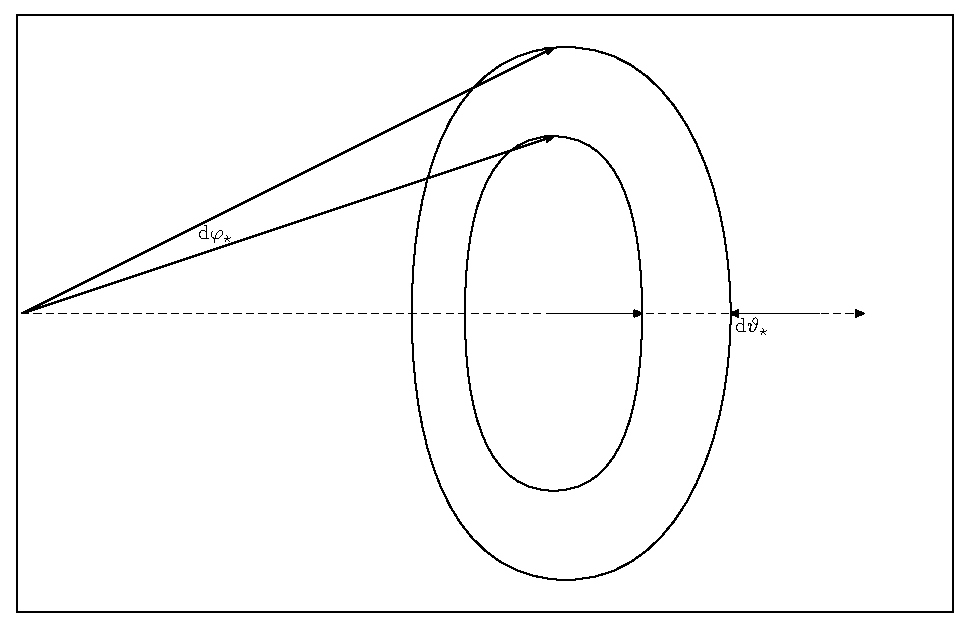
\includegraphics[height=6cm]{sezioneangolo.eps}
\caption{Sezione d'angolo solido \(\de \varphi\) e \(\de \vartheta\)
 sono invertiti rispetto alla figura} \label{fig:sezangolo}
\end{center}
\end{figure}

Con riferimento alla figura \vref{fig:sezangolo}, in $\cem$, la
probabilit\`a di trovare ua particella nell'angolo solido tra
$(\varphi^{\star},\varphi^{\star}+\de \varphi^{\star})$ e
$(\vartheta^{\star},\vartheta^{\star}+\de \vartheta^{\star})$ sono
indipendenti da $\varphi^{\star}$ e da $\vartheta^{\star}$
$$
\Longrightarrow \; \de \chi
(\varphi^{\star},\vartheta^{\star})=\frac{\de
\Omega(\varphi^{\star},\vartheta^{\star})}{4 \pi}.
$$
Per l'invarianza per rotazioni attorno all'asse $x$ si ha:
$$
\de \chi (\vartheta^{\star})=\int_{0}^{2 \pi}\frac{\de
\varphi^{\star} \;\de \cos \vartheta^{\star}}{4 \pi}=\frac{1}{2}
\de (\cos \vartheta^{\star})
$$
\`E poi cosa nota che:
\begin{equation}
E=(E^{\star}+c\beta p^{\star}\cos\vartheta^{\star})\gamma
\Longrightarrow \cos\vartheta^{\star}=\frac{E \sq
-E^{\star}}{c\beta p^{\star}} \label{eq:energiadeca}\end{equation}
da cui si ricava:
$$
\de \chi (E)=\frac{1}{2} \de (\frac{E \sq -E^{\star}}{c\beta
p^{\star}})=\frac{\de E}{2 c \beta p^{\star}\gamma}.
$$
Perci\`o in definitiva:
$$
\rho (E)=\frac{\de \chi (E)}{\de E}=\frac{1}{2}\frac{\sq}{c \beta
p_{\star}}
$$
Imponiamo in ultima le condizioni di normalizzazione:
$$
\int_{E_{\rem{min}}}^{E_{\rem{max}}} \rho (E)\,\de E=1:
\quad\mbox{ \`e una condizione plausibile?}
$$
Verifichiamolo:
\begin{equation}
\int_{E_{\rem{min}}}^{E_{\rem{max}}} \rho (E)\,\de E = \frac{1}{2 c
 \beta  p^{\star}\gamma}\,(E_{\rem{max}}-E_{\rem{min}})
\label{eq:distro}
\end{equation}
Ma, dalla (\ref{eq:energiadeca}), si ha:
$$
E_{\rem{max}}=(E^{\star}+c\beta p^{\star})\gamma
$$
ed:
$$
E_{\rem{min}}=(E^{\star}-c\beta p^{\star})\gamma
$$
da cui si ottiene che la (\ref{eq:distro}) diviene:
$$
\frac{1}{2}\frac{\sq}{c\beta p^{\star}}\gamma \,2 \,c \,\beta\,
p^{\star}=1,
$$
il che ci permette di concludere questa parte.
\subsection{ Urti tra particelle}
\footnote{ Usiamo la convenzione $c=1$} Per quanto rigurda i
processi d'urto tra particelle, nella nostra analisi, prenderemo
in considerazione solo urti elastici, ovvero urti dove le
particelle uscenti sono dello stesso tipo di quelle entranti. Per
focalizzare come avviene il processo d'urto tra due particelle,
possiamo riferirci alla figura \vref{fig:urto}.

\begin{figure}[htbp]
\begin{center}
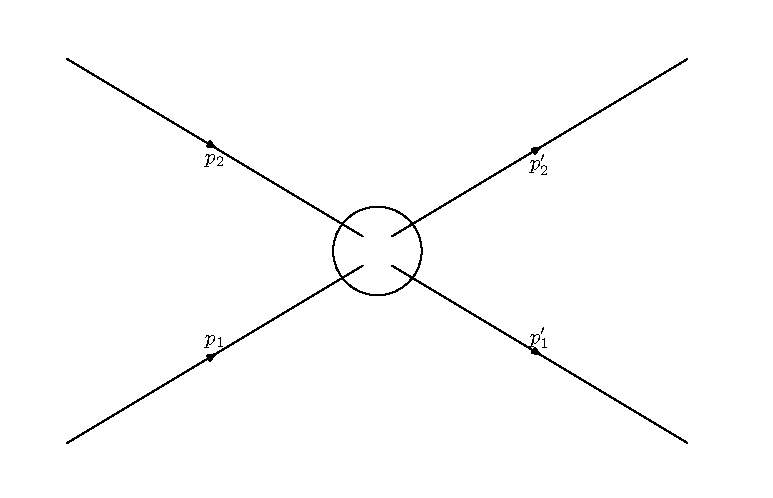
\includegraphics[width=10cm]{urto.eps}
\caption{Figura d'un urto elastico} \label{fig:urto}
\end{center}
\end{figure}

Quanti invarianti relativistici possiamo avere con tale processo?
Sappiamo che vale la conservazione del quadrimpulso, cio\`e che:
$$
p_1+p_2=p'_1+p'_2,
$$
il che implica:
$$
E_1+E_2=E'_1+E'_2, \quad\mbox{ un'equazione,}
$$
e
$$
\mathbf{p}_1+\mathbf{p}_2=\mathbf{p}_1{}'+\mathbf{p}_2{}',
\quad\mbox{ tre equazioni;}
$$
Inoltre abbiamo
$p_{{}_{1,2}}^2=m_{{}_{1,2}}^2=(p'_{{}_{1,2}}{})^2$, ovvero altre
quattro equazioni. Abbiamo dunque 8 condizioni sui sedici
parametri che compongono i 4 quadrimpulsi. Quindi si hanno altri 8
parametri liberi, che tuttavia scendono a due poich\`e possiamo
scegliere, mediante una rotazione e una trasformazione di Lorentz,
il sistema di riferimento che ci \`e pi\`u congeniale (e tale
operazione porta via altri 6 parametri). Vedremo pi\`u avanti cosa
rappresentano questi 2 parametri liberi.
\subsection{ Le variabili di Mandelstam}
\footnote{ Usiamo la convenzione $c=1$}
\index{Mandelstam!variabili di}Nello studio relativistico degli
urti tra particelle, sono state introdotte, da Mandelstam, quattro
invarianti relativistici, cos\`i definiti\footnote{\(s\) \`e anche detto
massa invariante, mentre \(t\) \`e anche detto momento invariante.}:
$$
s=(p_1+p_2)^2=(p'_1+p'_2)^2
$$
$$
t=(p_1-p'_1)^2=(p_2-p'_2)^2
$$
$$
u=(p_1-p'_2)^2=(p_2-p'_1)^2
$$
\begin{equation}
s+t+u=2(m_1^2+m_2^2). \label{eq:mandelstam}
\end{equation}
Non \`e difficile verificare la (\ref{eq:mandelstam}); infatti:
\begin{eqnarray*}
s+t+u & = & (p_1+p_2)^2+(p_1-p'_1)^2+(p_1-p'_2)^2\\ & =  & 3 p_1^2
+ p_2^2 + p'_1{}^2+p'_2{}^2 - 2 p_1 (p'_1 + p'_2 - p_2)
\end{eqnarray*}
dalla quale, ricordando che $p_1 + p_2 = p'_1 + p'_2$, e che
$p_i^2 = m_i^2$, si ottiene la (\ref{eq:mandelstam}). \newline
Possiamo ora specificare il dominio fisico di $s$, che risulta
essere $s\in[(m_1+m_2)^2,\infty]$; lo si verifica non troppo
difficilmente:
\begin{eqnarray*}
s & = & (p_1+p_2)^2\\
  & = & (p_1^{\star}+p_2^{\star})^2\\
  & \stackrel{\bigstar}{=} & (E_1^{\star}+E_2^{\star})^2\\
  & = & (\sqrt{p_{\star}^2 + m_1^2} + \sqrt{p_{\star}^2 +
  m_2^2})^2\\
  & \geq & (m_1 + m_2)^2
\end{eqnarray*}
L'unico passaggio che potrebbe necessitare delucidazioni \`e
$\bigstar$: chiariamo subito: nel CM valgono le relazioni:
\begin{equation}\left\{\begin{array}{ccc}
p_1^{\star} = (E_1^{\star},p^{\star},0,0)\\
p_2^{\star} = (E_2^{\star},-p^{\star},0,0)
\end{array}\right.\Longrightarrow |p_1^{\star} + p_2^{\star}| =
E_1^{\star} + E_2^{\star} \label{eq:abcd}
\end{equation}
e questo pu\`o essere sufficiente, a mio parere, per la
spiegazione.
\newline
Scriviamo poi un'altra relazione che ci torner\`a utile, tra le
altre cose, per la caratterizzazione del dominio fisico di $t$;
per la conservazione di $p$ si ha (nel caso di due particelle che
si urtano):
$$
\mathbf{p}_1^{\star} + \mathbf{p}_2^{\star}=\mathbf{p}_1^{'\star}
+ \mathbf{p}_2^{'\star}=\mathbf{0}
$$
$$
\Longrightarrow
$$
$$
p_{\star}=|\mathbf{p_{1}^{\star}}|=|\mathbf{p_{2}^{\star}}| \quad
\& \quad
p'_{\star}=|\mathbf{p_{1}^{'\star}}|=|\mathbf{p_{2}^{'\star}}|;
$$
Applicando la conservazione dell'energia:
$$
E_1^{\star} + E_2^{\star} = E_1^{'\star} + E_2^{'\star}
$$
$$
\Longrightarrow
$$
$$
\sqrt{p_{\star}^2 + m_1^2} + \sqrt{p_{\star}^2 +
  m_2^2} = \sqrt{p_{\star}^{'2} + m_1^2} + \sqrt{p_{\star}^{'2} +
  m_2^2}
$$
Tale relazione vale $\Leftrightarrow$ $p_{\star}=p'_{\star}$.
Ci\`o implica che:
$$
|\mathbf{p_{1}^{\star}}| = |\mathbf{p_{2}^{\star}}| =
|\mathbf{p_{1}^{'\star}}| = |\mathbf{p_{2}^{'\star}}| = p_{\star}
$$
Possiamo a questo punto caratterizzare $t$:
$$
t = (p'_1-p_1)^2 = (E_1^{'\star} - E_1^{\star})^2 -
(\mathbf{p}_1^{'\star} - \mathbf{p}_1^{\star})^2 =
$$
$$
0 - 2 p_{\star}^2(1 - \cos \vartheta_{\star}) \leq 0 \quad
(\rem{infatti }\;\; E_1^{'\star} = \sqrt{m_1^2 +
p_{\star}^2}=E_1^{\star}, \rem{ e }
p'_1=p^{\star}\cos\vartheta^{\star})
$$
Da queste due caratterizzazioni e da $ s + t + u = 2 (m_1^2 +
m_2^2)$, ne esce che l'intervallo fisico di $u$ \`e determinato da
$m_1$ ed $m_2$.
\subsection{ Gli urti veri e propri}
\footnote{ Usiamo la convenzione $c=1$} Ora che abbiamo introdotto
le variabili di Mandelstam, siamo in possesso di invarianti utili
alla formalizzazione del processo di urti tra particelle.
Prendiamo in considerazione l'urto in figura \vref{fig:urto}, tra
la particella 1, che, prima dell'urto, in $\lab$, ha quadrimpulso
pari a:
$$
p_1=(E_1,\mathbf{p}_1)
$$
e la particella 2, ferma in $\lab$, e che dunque ha quadrimpulso:
$$
p_2=(m_2,\mathbf{0}).
$$
Indichiamo con l'apice le quantit\`a dopo l'urto, e senz'apice le
quantit\`a prima dell'urto. La conservazione dell'energia in
$\lab$ implica:
\begin{equation}
E_1 + m_2 = E'_1 + E'_2 \longrightarrow E'_1 - E_1 = m_2 - E'_2.
\label{eq:energia_urto}
\end{equation}
Calcoliamoci gli invarianti relativistici:
\footnote{Ricordarsi che $p_i^2 = m_i^2$}
\begin{eqnarray*}
s_{\lab} &=& m_1^2 + m_2^2 + 2 (E_1 E_2 - \mathbf{p_1}\mathbf{p_2})\\
& \stackrel{E_2 = m_2,\;\; \mathbf{p_2}=\mathbf{0}}{=} & m_1^2 +
m_2^2 + 2 m_2 E_1
\end{eqnarray*}
\begin{eqnarray*}
t_{\lab} & = &  (p'_1-p_1)^2 \\ & = & (p'_2-p_2)^2  \\ & = & 2
m_2^2 -2 (E'_2 E_2 - \mathbf{p'_2}\mathbf{p_2})  \\ & \stackrel{
E_2 = m_2,\;\;\mathbf{p_2} = \mathbf{0} }{=} & 2 m_2^2 - m_2 E'_2 \\
& = & 2 m_2 (m_2 - E'_2) \\ &
\stackrel{(\ref{eq:energia_urto})}{=} & 2 m_2 (E'_1 - E_1).
\end{eqnarray*}
Ora sfruttiamo il fatto che $s_{\lab}=s_{\cem}$, ottenendo
(ricorda (\ref{eq:abcd})):
$$
\left(\sqrt{p_{\star}^2 + m_1^2} + \sqrt{p_{\star}^2 +
m_2^2}\right)^2 = m_1^2 + m_2^2 + 2 m_2 E_1
$$
$$
p_{\star}^2 + m_1^2 + p_{\star}^2 + m_2^2 + 2 \sqrt{p_{\star}^2 +
m_1^2}  \sqrt{p_{\star}^2 + m_2^2} = m_1^2 + m_2^2 + 2 m_2 E_1
$$
Semplificando:
$$
\sqrt{p_{\star}^2 + m_1^2}  \sqrt{p_{\star}^2 + m_2^2} = ( m_2 E_1
- p_{\star}^2)
$$
Elevando al quadrato otteniamo:
$$
p_{\star}^4 + p_{\star}^2 (m_1^2 + m_2^2) + m_1^2  m_2^2 = m_2^2
E_1^2 + p_{\star}^4 - 2 p_{\star}^2 m_2 E_1
$$
$$ p_{\star}^2 = \frac{m_2^2 (E_1^2 - m_1^2)}{m_1^2 + m_2^2 + 2
m_2 E_1}:
$$
$$\quad\mbox{\textsc{ho trovato} } p_{\star} \mbox{ \textsc{in funzione di
}} E_1.
$$
Vale poi $t_{\lab}=t_{\cem}$, ovvero:
$$
-2 p_{\star}^2 (1 - \cos\vartheta^{\star}) = 2 m_2 (E'_1 - E_1)
$$
$$
\Longrightarrow
$$
\begin{eqnarray*}
E'_1 & = & -\frac{2 p_{\star}^2}{2 m_2} (1-\cos \vartheta_{\star})
+ E_1\\
& = & -\frac{ p_{\star}^2}{ m_2} (1-\cos \vartheta_{\star}) + E_1\\
\end{eqnarray*}
Ora anche $E'_1$ \`e noto in funzione di $E_1$ e
$\vartheta_{\star}$. A questo punto $E'_{1_{max}}$ ed
$E'_{1_{min}}$ si ricavano facilmente. $E'_{1_{max}}= E'_1(\cos
\vartheta_{\star} = 1)$, e dunque $E'_{1_{max}}= E_1$. Invece:
$$
E'_{1_{min}} = \frac{E_1 (m_1^2 + m_2^2) + 2 m_2 m_1^2}{m_1^2 +
m_2^2 + 2 E_1 m_2}.
$$
\begin{observazione}
In fisica relativistica \`e possibile trasferire energia, anche in
quantit\`a molto grande, da una massa $m_1<<m_2$, alla massa
$m_2$, cosa che non era prevista prima. Infatti, nella condizione
$m_1<<m_2$:
$$
\frac{E'_{k\,\rem{min}_1}}{E_{k\,\rem{min}_1}}
\stackrel{m_1<<m_2}{\longrightarrow} \frac{m_2}{m_2 + E_1}
\stackrel{E_1 \rightarrow \infty}{\longrightarrow} 0.
$$
In fisica non relativistica invece $E - m \approx m v^2 / 2$,
$v^2<<c^2$ e perci\`o $E_1 m_2 \approx m_1 m_2$. Allora:
$$
\frac{E'_{k\,\rem{min}_1}}{E_{k\,\rem{min}_1}} \stackrel{v/c
<<1}{\approx} \frac{(m_1-m_2)^2}{m_1 + m_2} \stackrel{m_1 <<
m_2}{\longrightarrow} 1,
$$
come si voleva mostrare.
\end{observazione}
Se ora vogliamo stabilire come si dispongono gli impulsi dopo
l'urto, si procede analogamente a come proceduto nel decadimento,
sapendo il risultato della somma vettoriale $\mathbf{p'_1} +
\mathbf{p'_2} = \mathbf{p_1}$.
\newline
Ne esce dunque l'equazione dell'ellisse:
$$
\frac{ (p'_{y\,\alpha})^2 }{ p_{\star}^2 } + \frac{ 1- \beta^2 }{
p_{\star}^2 } \left( p'_{x\,\alpha} - \frac{ \beta
E_{\alpha}^{\star} }{ \sqrt{ 1 - \beta^2} }\right)^2 = 1.
$$
Si lascia al lettore farsi i vari casi, come nel decadimento.







%

\chapter{Elettromagnetismo}
\minitoc In questa dispensa ci siamo occupati, finora, di ridefinire
la dinamica e la meccanica classica, e i risultati sono stati dinamica
e meccanica relativistica. In questo capitolo ci occuperemo non di
ridefinire l'elettromagnetismo, in quanto esso gi\`a rispetta il
principio di relativit\`a einsteiniano, bens\`i di darne la sua
formulazione covariante.  Procedendo, inoltre, andremo incontro ad una
nuova unificazione concettuale di campo elettrico e campo magnetico,
in quanto saranno due lati diversi di uno stesso oggetto rappresentato
dal tensore del campo elettromagnetico\index{campo!elettromagnetico}.

\section{Il sistema di Gauss}
Per affrontare la nostra trattazione, introduciamo le equazioni di
Maxwell nel sistema di Gauss\index{equazioni!di Maxwell}:
\begin{equation}
  \mathbf{\nabla \cdot B } = 0, \label{eq:divergenzab}
\end{equation}
la quale \`e omogenea ed esprime che la divergenza del campo magnetico
\`e sempre pari a 0. Abbiamo poi:
\begin{equation}
  \mathbf{\nabla \times E } + \frac{ \partial \mathbf{B}}{ \partial
    x^0 } = 0. \label{eq:rotoree}
\end{equation}
Tale equazione \`e omogenea ed esprime l'irrotazionalit\`a del campo
elettrico, a meno di una variazione temporale del campo
magnetico. Invece
\begin{equation}
  \mathbf{\nabla \cdot E }  = 4 \pi \rho \label{eq:divergenzae}
\end{equation}
non \`e equazione omogenea invece, ed afferma che la sorgente del
campo elettrico \`e la densit\`a di carica. In ultima:
\begin{equation}
  \mathbf{\nabla \times B } = \frac{ \partial \mathbf{E}}{ \partial
    x^0 } + \frac{ 4 \pi }{c} \mathbf{ j } \label{eq:rotoreb}
\end{equation}
non omogenea; essa afferma che il rotore del campo magnetico \`e
dovuto alla variazione temporale del campo elettrico, ed alla
densit\`a di corrente.  \newline Dalla (\ref{eq:divergenzab}) ne esce:
\begin{equation}
  \mathbf{B} = \mathbf{\nabla \times A}, \label{eq:rotorea}
\end{equation}
nella quale $A$ \`e il potenziale \index{potenziale!generalizzato}
generalizzato di $B$. Usando nella (\ref{eq:rotoree}) tale equazione
ottengo:
\begin{equation}
  \mathbf{\nabla} \times \left(\mathbf{E} + \frac{\partial
      \mathbf{A}}{\partial x^0}\right) = 0. \label{eq:rotoreepiua}
\end{equation}
Da questa ricavo l'esistenza di un potenziale \index{potenziale!del
  campo elettrico}scalare $\varphi$ t.c.:
\begin{equation}
  \mathbf{E} = - \mathbf{\nabla} \varphi - \frac{ \partial
    \mathbf{A}}{\partial x^0}. \label{eq:potenzialee}
\end{equation}

\section{Il tensore $F^{\mu\nu}$}
Ci occupiamo in questa sezione di introdurre il tensore $F^{\mu\nu}$,
che racchiude in s\`e campo elettrico e magnetico. La sua comodit\`a
sta nel fatto che, dopo averlo scritto in un sistema di riferimento,
\`e possibile conoscerne la forma in qualsiasi altro sistema,
applicandovi le opportune matrici. Per comiciare osserviamo che
$\bef{B}$ e $\bef{E}$ sono invarianti sotto trasformazioni di
$\bef{A}$ e $\varphi$, fatte in tale modo ($\la$ \`e una funzione non
meglio specificata per ora):
\begin{equation}
  \begin{array}{cccccl}
    \bef{A} & \longrightarrow & \bef{A'} & = & \bef{A} - \bef{\nabla} \la &\\
    \varphi & \longrightarrow & \varphi' & = & \varphi +
    \partial_0 \la &
  \end{array},
  \label{eq:gauge}
\end{equation}
chiamate trasformazioni di gauge\index{trasformazioni!di gauge}.
\newline Poich\'e $\partial_0 = \partial^0 $, e $ - \bef{ \nabla } =
\partial^i = g^{i\mu}\partial_{\mu}$, e dacch\'e $\partial^{\mu}$ \`e
un quadrivettore controvariante, la (\ref{eq:gauge}) suggerisce che $
( \varphi , \bef{A} ) = A^{\mu} $, siano le quattro componenti di un
quadrivettore controvariante che trasforma per gauge; infatti, se
nella seguente equazione $\partial^{\mu}\la$ \`e un quadrivettore (il
che accade se \la \ \`e uno scalare), per consistenza anche $A^{\mu}$
dev'essere un quadrivettore:
$$
A^{'\mu} = A^{\mu} + \partial^{\mu}\la.
$$
A questo punto possiamo dare la:
\begin{definizione}[Quadritensore $F^{\mu\nu}$]
  Il tensore di rango due controvariante $F^{\mu\nu}$ \`e definito da
$$
F^{\mu\nu} = \partial^{\mu}A^{\nu} - \partial^{\nu}A^{\mu}.
$$
\end{definizione}
\begin{osservazione}
  \f \ \`e anti-simmetrico, e che:
$$
F^{i0} = \partial^i A^0 - \partial^0 A^i = -\frac{\partial
  \varphi}{\partial x^i} - \frac{\partial A^i}{\partial x^0} = E^i.
$$
Inoltre:
$$
F^{12} = - \frac{\partial A^2}{\partial x^1} + \frac{\partial
  A^1}{\partial x^2} = - (\bef{\nabla \times A})_3 = - B_3,
$$
ed analogamente:
$$
F^{23} = - B_1;
$$
a questo punto si intuisce la regola (che il lettore incredulo potr\`a
``sperimentalmente'' controllare):
\begin{equation}
  F^{ij} = - \varepsilon^{ijk}B_{k} \label{eq:fepsilon}
\end{equation}
e dunque:
\begin{equation}
  \f= \left(
    \begin{array}{cccc}
      0    &  -E_1  &  -E_2  &  -E_3 \\
      E_1  &    0   &  -B_3  &   B_2 \\
      E_2  &   B_3  &    0   &  -B_1 \\
      E_3  &  -B_2  &   B_1  &    0  \\
    \end{array}
  \right).
\end{equation}
Invece $F_{\mu\nu} = g_{\rho \mu} g_{\nu \sigma} F^{\rho \sigma}$.
\end{osservazione}
Enunciamo e dimostriamo ora delle importanti proposizioni:
\begin{proposizione}
  L'equazione $ \varepsilon_{\mu\nu\rho\sigma}
  \partial^{\nu} F^{\rho\sigma} = 0 $ \`e equivalente
  alla~(\ref{eq:divergenzab}) e alla~(\ref{eq:rotoree}).
\end{proposizione}
\begin{dimostrazione}
  Mostriamo innanzi tutto che $ \varepsilon_{\mu\nu\rho\sigma}
  \partial^{\nu} F^{\rho\sigma} = 0 $, e poi facciamo vedere la sua
  equivalenza con le due equazioni di Maxwell in esame. Si ha:
  \begin{eqnarray*}
    \varepsilon_{\mu\nu\rho\sigma}
    \partial^{\nu} F^{\rho\sigma} & = & \varepsilon_{\mu\nu\rho\sigma}
    \partial^{\nu}(\ff{\rho}{\sigma}) \\
    & \stackrel{\mbox{\tiny cambio nomi agli indici}}{=} &
    \varepsilon_{\mu\nu\rho\sigma}
    \partial^{\nu}
    \partial^{\rho} A^{\sigma} - \varepsilon_{\mu\nu\sigma\rho} \partial^{\nu}
    \partial^{\rho} A^{\sigma} \\
    & \stackrel{\mbox{\tiny per le propriet\`a di } \varepsilon}{=} &
    2 \varepsilon_{\mu\nu\rho\sigma}
    \partial^{\nu}
    \partial^{\rho} A^{\sigma}\\
    & = & 0
  \end{eqnarray*}
  L'ultima uguaglianza discende dal fatto che la contrazione di indici
  simmetrici (quelli delle derivate) con indici antisimmetrici (quelli
  di \f), d\`a 0, come si pu\`o facilmente verificare. Perci\`o
  $\varepsilon_{\mu\nu\rho\sigma}
  \partial^{\nu} F^{\rho\sigma} = 0$. Prendiamo $\mu = 0$; allora per
  la struttura di $\varepsilon_{ijkl}$, $\nu = i$, $\rho = j$, $\sigma
  = k$, e
  \begin{eqnarray*}
    \varepsilon_{0ijk} \partial^i F^{jk} & = & \varepsilon_{0123}
    \partial^1 F^{23} + \ldots\\
    & = & \frac{\partial ( -B_1 )}{\partial x^1} + \frac{\partial (
      -B_2 )}{\partial x^2} + \ldots \\
    & = & -2 \, \bef{\nabla \cdot B};
  \end{eqnarray*}
  Dunque abbiamo dimostrato che $\varepsilon_{\mu\nu\rho\sigma}
  \partial^{\nu} F^{\rho\sigma} = 0 \Longleftrightarrow \bef{\nabla
    \cdot B} = 0$. Passiamo ora alla seconda parte, prendendo in
  considerazione gli indici spaziali, ovvero sia $ \mu = 1,2,3 $.
  Allora:
  \begin{eqnarray*}
    \varepsilon_{iljk} \partial^l F^{jk} & = & \varepsilon_{i0jk}
    \partial^0 F^{jk} + \varepsilon_{ij0k}
    \partial^j F^{0k} + \varepsilon_{ijk0}
    \partial^j F^{k0} \\
    & = & - 2 \frac{\partial B_i}{\partial x^0} + 2 \varepsilon_{ijk0}
    \partial^j F^{k0} \\
    & = & - 2 \frac{\partial B_i}{\partial x^0} + 2
    \varepsilon_{ijk}\partial^j E_k \\
    & = & -2 \left[\frac{\partial B_i}{\partial x^0} + (\bef{\nabla
        \times E})_i \right],
  \end{eqnarray*}
  che \`e quanto si richiedeva.
\end{dimostrazione}
Segue ora un'importante
\begin{definizione}
  Il tensore quadricorrente \index{quadricorrente}$j^{\nu}$ \`e
  quell'oggetto le cui componenti sono $(c\rho, \bef{j})$, ove $\rho$
  \`e l'usuale densit\`a di carica\index{carica!densit\`a di}, e
  $\bef{j}$ \`e l'usuale densit\`a di corrente\index{densit\`a di
    corrente}.
\end{definizione}
Possiamo passare ora a dimostrare un'altra importante
\begin{proposizione}
  L'equazione $ \partial_{\mu} F^{\mu\nu} = j^{\nu}4 \pi /c $ \`e
  equivalente alla~(\ref{eq:divergenzae}) e alla~(\ref{eq:rotoreb}).
\end{proposizione}
\begin{dimostrazione}
  Prendiamo $\nu = 0$: allora $\mu = i$, e si ha:
$$
\partial_i F^{i0} = \partial_i E_i = \bef{\nabla \cdot E},
$$
che \`e quanto si richiede per la prima parte. Se invece $\nu = j$,
$\mu$ pu\`o essere sia spaziale che temporale. Dunque:
\begin{eqnarray*}
  \partial_{\mu}F^{\mu j} & = & \partial_0 F^{0j} + \partial_i F^{ij}\\
  & \stackrel{(\ref{eq:fepsilon})}{=} & - \frac{\partial E_j}{\partial x^0}
  - \frac{\partial }{\partial x^1}
  \varepsilon^{ijk}B_k\\
  & = & - \frac{\partial E_j}{\partial x^0}
  + (\bef{\nabla \times B})_i,
\end{eqnarray*}
il che ci permette di concludere.
\end{dimostrazione}
Come si sa, dalla (\ref{eq:divergenzae}), discende l'equazione di
continuit\`a e perci\`o deve valere il seguente
\begin{corollario}
  Da $\partial_{\mu} \f = j^{\nu}4 \pi /c$ discende l'equazione di
  continuit\`a.
\end{corollario}
\begin{dimostrazione}
  Infatti, moltiplicando ambo i membri di $\partial{\mu} \f = j^{\nu}4
  \pi /c$ per $\partial_{\nu}$ si ha, per contrazione di indici
  simmetrici con antisimmetrici:
$$
0 = \partial_{\nu}\partial_{\mu} \f = \partial_{\nu} j^{\nu}4 \pi /c;
$$
allora
$$
0 = \partial_{\nu} j^{\nu} = \partial_{0} j^{0} -
\partial_{i} j^{i} = \frac{\partial c \rho}{\partial c t} +
\bef{\nabla \cdot j} = \frac{\partial \rho}{\partial t} + \bef{\nabla
  \cdot j},
$$
da cui l'equazione di continuit\`a.
\end{dimostrazione}
\begin{proposizione}
  L'equazione di Lorentz \index{equazione!di Lorentz}per la
  carica\index{carica!in campo elettromagnetico} in campo
  elettromagnetico:
$$
\frac{\de \bef{p}}{\de t} = e \left[ \bef{E} + \frac{\bef{v}}{c}
  \times \bef{B}\right]
$$
e la legge di potenza per la carica in campo elettromagnetico:
$$
\frac{\de \mt{E}}{\de t} = e \, \bef{E \cdot v},
$$
sono equivalenti a:
$$
\frac{\de p^{\mu}}{\de s}=\frac{e}{c}\, \f u_{\nu}.
$$
\end{proposizione}
\begin{dimostrazione}
  Osserviamo che:
$$
\frac{\de p^{\mu}}{\de s} = \frac{\de p^{\mu}}{\de t}\frac{\gamma}{c};
$$
dunque dobbiamo innanzi tutto mostrare che:
$$
\frac{\de \bef{p}}{\de t}\frac{\gamma}{c} = \frac{\gamma}{c} \, e
\left[ \bef{E} + \frac{\bef{v}}{c} \times \bef{B}\right].
$$
Per farlo prendiamo la componente spaziale di $\f u_{\nu}$, ovvero
prendiamo $\mu = i$; allora:
$$
F^{i0}u_0 + F^{ij}u_j = \left[ E_i + (\frac{\bef{v}}{c} \times
  \bef{B})_i \right] \gamma,
$$
e ci\`o permette di concludere la prima parte. Per la seconda si ha:
$$
\frac{\de p^{0}}{\de s} = \frac{e}{c}\, F^{0i}u_i;
$$
allora:
$$
\frac{\de p^{0}}{\de t} = \frac{e}{c}\, \bef{E \cdot v},
$$
il che \`e equivalente, ricordando la (\ref{eq:quadrimpulso}), a
$$
\frac{\de \mt{E}}{\de t} = e \,\bef{E \cdot v}.
$$
\end{dimostrazione}
Ci domandiamo ora se \`e possibile costruire degli invarianti, o
scalari, utili con il tensore doppio \f. La risposta \`e nella:
\begin{proposizione}
  Gli scalari $F_{\mu\nu}\f$ ed
  $\varepsilon_{\mu\nu\rho\sigma}F^{\mu\nu}F^{\rho\sigma}$ sono
  invarianti, in quanto scalari (e sono scalari in quanto si ottengono
  dalla contrazione di indici covarianti con indici controvarianti), e
  valgono, rispettivamente,
$$
2(\bef{B^2-E^2})
$$
$$
-8 (\bef{E\cdot B}).
$$
\end{proposizione}
\begin{dimostrazione}
  Si verificano entrambi con un semplice calcolo:
  \begin{eqnarray*}
    F_{\mu\nu}\f & = & F_{0i}F^{0i} + F_{i0}F^{i0} + \ldots \\
    & = & 2 (-E_i^2 + B_i^2)\\ & = & 2 (\bef{B^2-E^2});
  \end{eqnarray*}
  \begin{eqnarray*}
    \varepsilon_{\mu\nu\rho\sigma}F^{\mu\nu}F^{\rho\sigma} & = &
    \varepsilon_{0123}F^{01}F^{23} + \ldots \\
    & = & 8 (\mbox{}-E_1 B_1 - E_2 B_2 -E_3 B_3)\\
    & = & -8 (\bef{E\cdot B}).
  \end{eqnarray*}
\end{dimostrazione}

\section{\f \ sotto trasformazioni di Lorentz}
In questa sezione andiamo ad analizzare come il tensore
elettromagnetico \f \ cambia sotto trasformazioni di Lorentz.  Essendo
un tensore controvariante di rango 2, esso trasformer\`a, sotto $\la
\in \mt{L}_{+}^{\uparrow}$ in questo modo:
\begin{displaymath}
F^{'\mu\nu}(\bef{x}') = \la^{\mu}{}_{\rho}\la^{\nu}{}_{\sigma}
F^{\rho\sigma}(\bef{x}),
\end{displaymath}
dove $\bef{x}'=\la \bef{x}$. Se \la \ rappresenta una trasformazione
propria di Lorentz lungo $x$, allora:
\begin{displaymath}
\la = \left(
  \begin{array}{cccc}
    \gamma & - \beta \gamma & 0 & 0\\
    -\beta \gamma & \gamma & 0 & 0\\
    0&0&1&0\\
    0&0&0&1
  \end{array}
\right).
\end{displaymath}
Calcoliamoci qualche componente di \f \, per capire cosa e come
cambia:
\begin{eqnarray*}
  -E'_1  =  F^{'01} & = &
  \la^0{}_{\rho}\la^{1}{}_{\sigma}F^{\rho\sigma}\\
  & = & \la^0{}_{0}\la^{1}{}_{\sigma}F^{0\sigma} +
  \la^0{}_{1}\la^{1}{}_{\sigma}F^{1\sigma} \\
  & = & \la^0{}_{0}\la^{1}{}_{1}F^{01} +
  \la^0{}_{1}\la^{1}{}_{0}F^{10} \\
  & = & \left( \gamma^2 - \beta^2\gamma^2\right)F^{01}\\
  & = & F^{01} = -E_1,
\end{eqnarray*}
mentre, ad esempio, per una componente che non sia lungo l'asse delle
$x$:
\begin{eqnarray*}
  -E'_2  =  F^{'02} & = &
  \la^0{}_{\rho}\la^{2}{}_{\sigma}F^{\rho\sigma} \\
  & = & \la^0{}_{\rho}\la^{2}{}_{2}F^{\rho2}\\
  & = & \la^0{}_{0}\la^{2}{}_{2}F^{02} +
  \la^0{}_{1}\la^{2}{}_{2}F^{12} \\
  & =& \gamma F^{02} -\beta\gamma F^{12}\\
  & = & \gamma \left( -E_2 + \beta B_3 \right).
\end{eqnarray*}
Risparmiando al lettore (e a me), i calcoli di tutte le altre
componenti, riportiamo solo i risultati:
\begin{eqnarray*}
  E'_1 & = & E_1\\
  E'_2 & = & (E_2 - \beta B_3) \gamma\\
  E'_3 & = & (E_3 + \beta B_2) \gamma\\
  B'_1 & = & B_1\\
  B'_2 & = & (B_2 + \beta E_3) \gamma\\
  B'_3 & = & (B_3 - \beta E_2) \gamma.
\end{eqnarray*}
Cosa \`e possibile fare con questo risultato? Prendiamo in
considerazione $\bef{E}$ e $\bef{B}$ costanti. Si hanno quattro
possibilit\`a:
\begin{enumerate}
\item $\bef{E \cdot B} = 0$, con $\bef{B^2-E^2}<0$;
\item $\bef{E \cdot B} = 0$, con $\bef{B^2-E^2}=0$;
\item $\bef{E \cdot B} = 0$, con $\bef{B^2-E^2}>0$;
\item $\bef{E \cdot B} \neq 0$.
\end{enumerate}
Con opportune trasformazioni di Lorentz
\begin{enumerate}
\item porta a solo $\bef{E}$;
\item non porta a nessuna situazione interessante;
\item porta a solo $\bef{B}$;
\item porta a $\bef{E \sslash B}$.
\end{enumerate}
Vediamo come. Ricordando Lorentz lungo $x$, partiamo dalla 1; campo
elettrico e campo magnetico sono ortogonali, e
\begin{displaymath}
\frac{\bef{|B|}}{\bef{|E|}}<1;
\end{displaymath}
scelgo gli assi nella maniera pi\`u comoda, e precisamente tali che
$\bef{E} = (0,|\bef{E}|,0)$, $\bef{B} = (0,0,|\bef{B}|)$. Il risultato
che voglio ottenere da 1. \`e che $\bef{B'} = 0$ e ci\`o comporta:
\begin{equation}
  \left\{
    \begin{array}{ccccc}
      B_{y}' & = & B_y & = & 0\\
      B_{x}' & = & B_x & = & 0\\
      B_{z}' & = & \gamma(B_z - \beta E_y) & = & 0\\
    \end{array}.
  \right.
\end{equation}
Le prime due sono gi\`a soddisfatte, la terza \`e soddisfatta se
$\beta = |B_z|/|E_y|$, e la condizione \`e possibile poich\'e, per
ipotesi $|B_z|/|E_y|<1$ (e tale ipotesi deve valere perch\'e
$\beta<1$, ovvero affinch\'e la trasformazione esista.). Si lascia per
esercizio il dimostrare che da 3. si pu\`o arrivare ad una situazione
in cui ci sia solo $\bef{B}$, mentre si passa a far vedere che da
4. si pu\`o arrivare a campo magnetico parallelo a campo elettrico. Se
effettuo una trasformazione lungo l'asse delle $x$, posso prendere
$E'_x = E_x = 0$, e $B'_x = B_x = 0$. Deve poi valere:
\begin{displaymath}
\bef{E'\times B'}=0,
\end{displaymath}
che porta a:
\begin{equation}
  E'_y B'_z - E'_z B'_y = 0, \label{eq:eparallelob}
\end{equation}
pi\`u ad altre due equazioni che sono sempre vere se $E'_x = B'_x =
0$; la (\ref{eq:eparallelob}) d\`a:
\begin{eqnarray*}
  \gamma (E_y - \beta B_z)\gamma (B_z - \beta E_y) - \gamma (E_z -
  \beta B_y)\gamma (B_y - \beta E_z) & = & \\
  \mbox{} - \beta (\bef{B^2 + E^2}) + (1+\beta^2)(E_y B_z - E_z B_y)
  & = & 0
\end{eqnarray*}
e questa impone che debba valere
\begin{equation}
  \frac{\bef{E \times B}}{\bef{B^2 + E^2}} =
  \frac{\vec{\beta}}{1+\beta^2};
\end{equation}
il secondo membro di quest'equazione ha come dominio di $\beta$
l'intervallo $[0,1]$, e dunque come codominio $[0,0.5]$. Posso
trovarmi esplicitamente $\beta$ da questa relazione, ma \`e vero che
\begin{displaymath}
0 <\frac{|\bef{E \times B}|}{\bef{B^2 + E^2}}<\frac{1}{2}\,?
\end{displaymath}

Dacch\'e $|\bef{E \times B}|\leq |\bef{E}||\bef{B}|$, devo mostrare
che $2|\bef{E}||\bef{B}|\leq \bef{B^2 + E^2} $: ma \`e sempre vero,
poich\'e quanto appena scritto \`e vero essendo equivalente a:
\begin{displaymath}
\bef{|E| + |B|}\geq0,
\end{displaymath}
il che ci d\`a modo di concludere.
\section{ La $\delta$ di Dirac}\index{delta!di Dirac}
La fisica relativistica, come gi\`a accennato in precendenza, si
configura come campo di studio molto utile per descrivere le
interazioni tra particelle elementari. Tuttavia in relativit\`a non
esistono corpi rigidi\footnote{Si prenda una sfera di raggio $R$. Se
  essa fosse rigida, l'informazione di un colpo di un proiettile ad
  una sua estremit\`a, si propagherebbe istantaneamente all'altra sua
  estremit\`a, per la rigidit\`a del corpo. Questo tuttavia \`e
  impossibile per la finitezza della velocit\`a dell'informazione.}, e
quindi \`e comodo, e produce risultati in accordo con la pratica,
trattare ogni particella come puntiforme, in quanto \`e molto
difficoltoso considerare tutti i corpi come elastici. Tuttavia non \`e
rigoroso, dal punto di vista matematico, l'approssimazione
puntiforme. Si prenda infatti un elettrone dentro un volumetto $\de
V$, la cui posizione sia costantemente associata al vettore
$\bef{x}$. Se volessimo avere la funzione densit\`a di carica in
$\de\,V$, necessiteremmo di una funzione $\rho(\bef{z})$ identicamente
uguale a 0, tranne che per $\bef{z}=\bef{x}$. Integrando questa
funzione sul volumetto dovremmo trovare $e = - 1.6 \times 10^{-19}
C$. Ma l'integrale di una funzione quasi ovunque nulla d\`a 0, per
noti risultati dell'analisi matematica. Si dovette quindi introdurre
la cosiddetta $\delta$ di Dirac, che si pu\`o trattare come,
rigorosamente, un funzionale\footnote{Pi\`u precisamente di una
  distribuzione con dominio in $\mt{D^{*}}$.}, che ad ogni funzione
associa il valore della funzione nell'origine.  Dunque:
\begin{equation}
  <\delta,\varphi> = \varphi(0),
  \label{eq:fun_delta}
\end{equation}
se $\varphi \in C^{\infty}_C$\footnote{$C^{\infty}_C$ \`e lo spazio
  vettoriale delle funzioni infinitamente derivabili e a supporto
  compatto} e $\lim_{x\rightarrow\infty} \varphi^{(n)} = 0$; si pu\`o
alternativamente dire che la $\delta$ associa a $\varphi$ la funzione:
\begin{equation}
  \int_{\mathbb{R}} \, \delta (x) \, \varphi(x) \, \de  x =
  \varphi(0).
  \label{eq:int_delta}
\end{equation}
La $\delta$ di Dirac gode di alcune propriet\`a, che andiamo ad
elencare:
\begin{equation}
  \int \, \delta(x)\, \de  x = 1
\end{equation}
\begin{equation}
  \delta(x) = 0 \; \forall\,x \neq 0
  \label{eq:eg_delta}
\end{equation}
\begin{equation}
  \delta(x) = \infty \; \mbox{se } x=0.
  \label{eq:imp_delta}
\end{equation}
Vi \`e poi $\delta (x - a)$, che pu\`o dirsi il funzionale che opera
in tale maniera (la $\varphi$ soddisfa le ipotesi sopraelencate):
$$
<\delta_a,\varphi> = \varphi(a).
$$

Passiamo ora ad enunciare la
\begin{proposizione}
  \label{prop:derivata_delta}
  La derivata della $\delta$ \`e quel funzionale che opera in tal
  modo:
$$
<\delta', \varphi> = - \varphi'(0)
$$
\end{proposizione}
\begin{dimostrazione}
  \begin{eqnarray*}
    \int_{-\infty}^{+\infty} \frac{\de }{\de x}\delta(x) \varphi(x) \de
    x & = & [\delta(x)\varphi(x)]_{-\infty}^{+\infty} -
    \int_{-\infty}^{+\infty} \delta(x) \frac{\de}{\de x} \varphi(x)
    \de x
    \\
    & = &  0 - \int_{-\infty}^{+\infty} \delta(x) \frac{\de}{\de x}\,
    \varphi(x) \de x \\
    & = & - \frac{\de}{\de x} \, \varphi(0)
  \end{eqnarray*}
\end{dimostrazione}
A questo punto si possono estendere le propriet\`a a spazi
$n-$dimensionali. In particolare la $\delta$ 3-dimensionale \`e quel
funzionale t.c.
$$
<\delta^{(3)},\varphi> = \int_{\mathbb{R}^3} \varphi(\bef{x})
\delta^{(3)} (\bef{x-a}) \de x \, \de y \, \de z = \varphi(\bef{a}).
$$
Ora \`e chiaro che la densit\`a di carica dell'elettrone nel volumetto
pu\`o scriversi:
$$
\rho(\bef{x}) = e \, \delta^{(3)}(\bef{x-z}),
$$
dove $\delta^{(3)}(\bef{x-z}) = \delta(x^1-z^1) \, \delta(x^2-z^2) \,
\delta(x^3-z^3)$, e $\varphi (x) = \chi_{\scriptscriptstyle \de V}(x)$
(vale 1 se $x \in \de V$, 0 altrimenti). Si estende in maniera
naturale agli spazi con pi\`u dimensioni.
\begin{observazione}
  In realt\`a non \`e corretto affermare $\delta(0)= + \infty$, n\'e
  ha molto senso l'integrale (\ref{eq:int_delta}), per i motivi
  ricordati prima, ovvero che una funzione che sia nulla quasi ovunque
  non pu\`o avere integrale di Lebesgue non nullo: l'unica notazione
  che ha senso \`e la (\ref{eq:fun_delta}), che definisce la $\delta$,
  come funzionale: la funzione rappresentativa $\delta(x)$ ha senso
  solo per $x \neq 0$ (ovvero la \ref{eq:eg_delta}); inoltre usare la
  funzione rappresentativa \`e comodo, come si \`e potuto constatare
  nella dimostrazione della proposizione
  \ref{prop:derivata_delta}. Per motivi storici, tuttavia, ho
  preferito scrivere la (\ref{eq:imp_delta}), giustificando qui, per
  correttezza, la mia scelta.
\end{observazione}
\section{ La quadridensit\`a di corrente}
Abbiamo gi\`a definito prima la quadridensit\`a di corrente in termini
di $c\rho$ e $\bef{j}$, grandezze che, alla luce dell'introduzione
della $\delta$ di Dirac possono essere riscritte, se $\bef{z}(x^0)$
rappresenta un moto parametrizzato dal tempo, in tale maniera
$$
c\rho (\bef{x},x^0)= e \, c \, \delta^{(3)}(\bef{x-z(x^0)}),
$$
$$
\bef{j} (\bef{x},x^0) = e\,c \frac{\de \bef{z}}{\de x^0}
\delta^{(3)}(\bef{x-z(x^0)}) = \rho (\bef{x},x^0) \bef{v};
$$
dunque
$$
j^{\mu} = (c\rho,\bef{v} \rho) = e\,c \frac{\de z^{\mu}}{\de x^0}
\delta^{(3)}(\bef{x-z(x^0)}) = \rho \frac{\de z^{\mu}}{\de x^0}
$$
se $z^{\mu}(x^0) = (x^0 , \bef{z}(x^0))$; a questo punto \`e anche
possibile scrivere
\begin{equation}
  j^{\mu} = e\,c\int_{-\infty}^{+\infty} \de s \,\frac{\de
    z^{\mu}}{\de s} \delta^{(4)}(x-z(s)), \label{eq:quadricorrente}
\end{equation}
dove $s$ \`e il parametro per il moto $z^{\mu}$; si pu\`o subito
controllare che la (\ref{eq:quadricorrente}) \`e consistente con le
definizioni date sinora; infatti:
$$
j^{i} = e\,c \int_{-\infty}^{+\infty} \de s \,\frac{\de z^{i}}{\de s}
\delta^{(3)}(\bef{x-z}(z^0))\delta(x^0 - z^0),
$$
dove $\delta(x^0 - z^0)$ ci fa valutare la nostra espressione in $z^0
= x^0$, che porge:
$$
j^{i} = e\,c \frac{\de z^i}{\de x^0}\delta^{(3)}(\bef{x-z}(x^0)),
$$
come si voleva; invece
$$
j^{0} = e\,c \int_{-\infty}^{+\infty} \de z^0
\delta^{(3)}(\bef{x-z}(z^0))\delta(x^0 - z^0) =
c\,e\,\delta^{(3)}(\bef{x-z}(x^0)).
$$

Ci vogliamo ora chiedere se $j^{\mu}$ sia un quadrivettore. Ci\`o \`e
assicurato dalla seguente
\begin{proposizione}
  $j^{\mu}(x)$ \`e un quadrivettore.
\end{proposizione}
\begin{dimostrazione}
  Per la dimostrazione abbiamo bisogno del seguente
  \begin{lemma}
    $\delta^{(4)}(Mx)=\delta^{(4)}(x)/|\det M|$, dove $M$ \`e una
    matrice $4 \times 4$.
  \end{lemma}
  \begin{dimostrazione}
    Dimostriamolo nel caso unidimensionale, e poi estendiamo il
    ragionamento a quattro dimensioni (senza dimostrazione). Sia $c
    \neq 0$; $\delta(cx) = \int \delta (cx) \varphi(x) \, \de x$:
    poniamo $cx=y$, in modo tale che l'integrale diviene
$$
\int \frac{1}{|c|}\,\delta(y)\,\varphi(\frac{y}{c})\,\de y =
\frac{1}{|c|}\varphi(0) = \frac{1}{|c|} <\delta,\varphi>.
$$
\end{dimostrazione}
Tornando alla nostra dimostrazione, se $j^{\mu}$ \`e un quadrivettore,
allora:
$$
j^{'\mu} = \la^{\mu}{}_{\nu}j^{\nu},\,\rem{x}'=\la \rem{x} \quad
\mbox{ con } \la \in \mt{L}_{+}^{\uparrow}.
$$
Vediamo se \`e vero.
\begin{eqnarray*}
  j^{'\mu} & = &  c\,e\int_{-\infty}^{+\infty} \de s \,\frac{\de
    z^{'\mu}}{\de s} \delta^{(4)}(x'-z'(s))\\
  & = & c\,e \int_{-\infty}^{+\infty} \de s \, \la^{\mu}{}_{\nu}
  \frac{\de
    z^{\nu}}{\de s} \delta^{(4)}(\la(x-z(s)))\\
  & = & c \, e \, \frac{\la^{\mu}{}_{\nu}}{|\det
    \la|}\int_{-\infty}^{+\infty} \de s \, \frac{\de z^{\nu}}{\de s}
  \delta^{(4)}(x-z(s))\\
  & = & \la^{\mu}{}_{\nu} \, c \, e \, \int_{-\infty}^{+\infty} \de
  s
  \, \frac{\de z^{\nu}}{\de s} \delta^{(4)}(x-z(s))\\
  & = & \la^{\mu}{}_{\nu} j^{\nu},
\end{eqnarray*}
come si richiedeva.
\end{dimostrazione}



Viene ora spontaneo chiedersi se anche dalla (\ref{eq:quadricorrente})
esce l'equazione di continuit\`a. La risposta viene dalla seguente
\begin{proposizione}
  $\partial_{\mu}j^{\mu} = 0$
\end{proposizione}
\begin{dimostrazione}
  Se $\partial_{\mu}j^{\mu} = 0$, integrando deve valere:
  \begin{equation}
    \int \de^4 x \varphi(x) \partial_{\mu}j^{\mu}(x) = 0
    \label{eq:continuitauno}
  \end{equation}
  per ogni $\varphi$ che posso scegliere tra quelle $\mt{C}^{\infty}$,
  e tali che siano a supporto compatto. Devo dunque mostrare che la
  validit\`a della (\ref{eq:continuitauno}); integrando per parti
  ottengo
$$
-\int \de^4 x j^{\mu}(x) \, \partial_{\mu}\varphi(x).
$$
Sostituendo $j^{\mu}$
\begin{eqnarray*}
  -\int \de^4 x  \int_{-\infty}^{+\infty} \de s \frac{\de
    z^{\mu}}{\de s} \delta^{(4)}(x-z(s))
  \partial_{\mu}\varphi(x)
  & = & \\
  -\int_{-\infty}^{+\infty} \int \de^4 x\, \,\delta^{(4)}(x-z(s))\,
  \frac{\partial \varphi(x)}{\partial x^{\mu}} \de s \frac{\de
    z^{\mu}}{\de s} & = & \\
  -\int_{-\infty}^{+\infty} \frac{\partial\varphi(s)}{\partial
    z^{\mu}}\, \de s \frac{\de z^{\mu}}{\de s} & = & \\
  -\int_{-\infty}^{+\infty} \de s \frac{\de \varphi(s)}{\de s}
  & = & \\
  -\left[ \varphi(z)\right]_{z=-\infty}^{z=+\infty};
\end{eqnarray*}
l'ultimo termine va a 0 tuttavia, poich\`e $\varphi$ \`e a supporto
compatto, e possiamo cos\`i concludere.
\end{dimostrazione}


\section{ Moti di particelle}
Ci proponiamo in questa sezione, tramite due esempi, di studiare il
moto di particelle elementari immerse in campo elettrico e
magnetico. Indicheremo con $\mt{E}$ l'energia, e con $E$ il campo
elettrico.

\begin{esempio}
  Consideriamo una particella immersa in un campo magnetico costante,
  in assenza di campo elettrico, e sia $c = 1$. Le equazioni che
  regolano il moto della particella sono:
  \begin{equation}
    \frac{\de \bef{p}}{\de t} = \frac{e}{c} \bef{v \times B}
    \label{eq:lorentzesempio}
  \end{equation}
$$
\frac{\de \mt{E}}{\de t} = e \bef{E \cdot v} \stackrel{\bef{E}=0}{=}
0;
$$
dall'ultima vediamo che l'energia si conserva, essendo la sua derivata
rispetto al tempo nulla; consideriamo che:
\begin{equation}
  \bef{v} = \frac{\bef{p}}{\mt{E}};
\end{equation}
sostituendo tale equazione nella (\ref{eq:lorentzesempio}) otteniamo:
\begin{equation}
  \mt{E}\frac{\de \bef{v}}{\de t} = \frac{e}{c}\bef{v \times B};
  \label{eq:lorenzesempiouno}
\end{equation}
da questa vedo che $\bef{|v|}$ \`e costante; difatti, moltiplicando
membro a membro per $\bef{v}$
\begin{eqnarray*}
  \bef{v}\mt{E}\frac{\de \bef{v}}{\de t} & = &
  \frac{e}{c}\bef{v\cdot (v \times B)}\\
  & \mbox{da cui} & \\
  \frac{\mt{E}}{2} \frac{\de \bef{v^2}}{\de t} & = & 0;
\end{eqnarray*}
scegliamo ora gli assi in modo che il campo magnetico sia parallelo
all'asse $z$. Essendo $\bef{B} = (0,0,B)$, dalla
(\ref{eq:lorenzesempiouno}) discende:
$$
\dot{v}_x = \frac{e B}{\mt{E}}v_y,
$$
$$
\dot{v}_y = -\frac{e B}{\mt{E}}v_x,
$$
$$
\dot{v}_z = 0;
$$
per risolver\`o usiamo il metodo suggerito in~\cite{gdmdue}, capitolo
11, il quale propone, nel caso si abbia il sistema
$$
\left\{
  \begin{array}{ccc}
    \dot{x} & = & a_t x - b_t y + \alpha_t \\
    \dot{y} & = & b_t x + a_t y + \beta_t,
  \end{array}
\right.
$$
dove $a,\,b,\,\alpha,\,\beta$ sono funzioni continue su un certo
intervallo $I$, e a valori in $\mathbb{R}$, e dove il pedice $t$
indica la dipendenza dal parametro $t\in I$, di porre $z = x + i y,
c_t = a_t + i b_t, \gamma_t = \alpha_t + i \beta_t $, in maniera tale
da ricondursi a
$$
\dot{z} = c_t z + \gamma_t;
$$
perci\`o per le nostre equazioni la soluzione \`e:
$$
v = v(0) e^{-i\omega t},
$$
dove $v = v_x + i\, v_y$ e $\omega = e B / \mt{E}$; dunque:
$$
v = v_0 e^{-i\alpha}e^{-i\omega t},
$$
e
$$
\frac{\de x}{\de t} = v_x(t) = v_0 \cos(\omega t - \alpha),
$$
$$
\frac{\de y}{\de t} = v_y(t) = v_0 \sin(\omega t + \alpha).
$$
Da queste e dall'equazione su $v_z(t)$
\begin{equation}
  x - k_1 = \frac{v_0}{\omega} \sin(\omega t - \alpha),
  \label{eq:kappa1}
\end{equation}
\begin{equation}
  y - k_2 = \frac{v_0}{\omega} \cos(\omega t + \alpha),
  \label{eq:kappa2}
\end{equation}
$$
z = z_0 + v_{0z}t,
$$
dove $k_1,\,k_2$ sono costanti da determinare a seconda delle
condizioni iniziali; osserviamo che quadrando e sommando la
(\ref{eq:kappa1}) e la (\ref{eq:kappa1}) si ottiene l'equazione di una
circonferenza di raggio $v_0/\omega$ e centro $(k_1,k_2)$, ovvero:
$$
(x - k_1)^2 + (y - k_2)^2 = \frac{v_0^2}{\omega^2}.
$$
\end{esempio}

\begin{esempio}
  Consideriamo una particella immersa in un campo elettrico costante,
  in assenza di campo magnetico, e sia $c = 1$. Le equazioni che
  regolano il moto della particella sono:
$$
\frac{\de \bef{p}}{\de t} = e \bef{E},
$$
con $\bef{p}$ impulso relativistico. Scelgo l'asse delle $x$ in modo
che $\bef{E}=(E,0,0)$, e l'asse delle $y$ in modo che $\bef{p}(o)$ ed
$\bef{E}$ stiano sul piano formato da $x$ e $y$.  Ho dunque:
$$
\begin{array}{ccc}
  p_x(0) = p_{0x} & p_y(0) = p_{0y} & p_z(0) = 0,\\
  % & \stackrel{\mbox{ }}{\mbox{}} & \\
  \dot{p}_x = e E & \dot{p}_y = 0 & \dot{p}_z = 0 \\
  & \Longrightarrow & \\
  p_x= e E t + p_{0x} & p_y = p_{0y} & p_z = p_{0z} = 0;
\end{array}
$$
scelgo ora l'origine dei tempi in modo che $p_{0x} = 0$ (posso sempre
farlo, basta prendere $t' = t + p_{0x}/(e E)$); in tal modo
$$
p_x = e E t;
$$
per ottenere la velocit\`a
$$
\bef{v} = \frac{\bef{p}}{\mt{E}},
$$
dove
$$
\mt{E} = \sqrt{m^2 + \bef{p}^2} = \sqrt{m^2 + p_{0y}^2 + (e E t)^2}
\stackrel{\mt{E}_0^2 = m^2 + p_{0y}^2}{=} \sqrt{\mt{E}_0^2 + (e E
  t)^2},
$$
da cui:
$$
\bef{v} = \frac{\bef{p}}{\mt{E}} = \left( \frac{e E
    t}{\sqrt{\mt{E}_0^2 + (e E t)^2}}, \frac{p_{0y}}{\sqrt{\mt{E}_0^2
      + (e E t)^2}}, 0\right).
$$
Osservo che:
$$
\frac{e E t}{\sqrt{\mt{E}_0^2 + (e E t)^2}} = \frac{1}{e E}
\frac{\de}{\de t}\sqrt{\mt{E}_0^2 + (e E t)^2},
$$
e questo mi permette di scrivere:
$$
\frac{\de x}{\de t} = \frac{1}{e E} \frac{\de}{\de t}\sqrt{\mt{E}_0^2
  + (e E t)^2};
$$
allora
$$
x - x_0 = \frac{1}{e E}\left( \sqrt{\mt{E}_0^2 + (e E t)^2} -
  \mt{E}_0\right);
$$
invece
$$
\frac{\de y}{\de t} = \frac{p_{0y}}{\sqrt{\mt{E}_0^2 + (e E t)^2}} =
\frac{p_{0y}}{e E} \frac{\de}{\de t} \asinh\left( \frac{e E
    t}{\mt{E}_0}\right),
$$
dalla quale
$$
y - y_0 = \frac{p_{0y}}{e E} \asinh\left( \frac{e E
    t}{\mt{E}_0}\right);
$$
facciamo notare che la forza relativistica non \`e parallela alla
velocit\`a, dunque anche lungo $y$ ce n'\`e.

Per trovare la traiettoria poniamo
$$
\alpha = (y - y_0) \frac{e E}{p_{0y}},
$$
in modo da poter scrivere
\begin{equation}
  \sinh \alpha = \frac{e E t}{\mt{E}_0}. \label{eq:traiettoriae}
\end{equation}
Allora:
\begin{eqnarray*}
  e E (x - x_0) &\stackrel{\cosh \alpha \mbox{ per
      (\ref{eq:traiettoriae})}}{=}& \mt{E}_0 \left(\sqrt{ 1 +
      \left(\frac{e E t}{\mt{E}_0}\right)}\right) \\ & = & \mt{E}_0
  (\cosh \alpha - 1)  \\ & = & \mt{E}_0 (\cosh (y - y_0  \frac{e
    E}{p_{0y}}) - 1),
\end{eqnarray*}
e questa \`e la traiettoria; il limite non relativistico \`e quello
dove la traiettoria \`e una parabola; infatti per $c \rightarrow
\infty$:
$$
\alpha \rightarrow 0
$$
(dacch\'e al denominatore di $\alpha$ vi \`e $c$, se esso \`e diverso
da 1), e
$$
\cosh \alpha \rightarrow 1 + \frac{\alpha^2}{2},
$$
che porta a
$$
e E (x- x_0) \approx \mt{E}_0 \frac{1}{2} \left[ \frac{(y - y_0) e
    E}{p_{0y} c } \right]^2;
$$
nel limite $c \rightarrow \infty$, $\mt{E}_0 \approx mc^2$, $p_{0y}
\approx m v_0$, e
$$
(x- x_0) \approx \frac{1}{2} \frac{e E}{m v_0^2}(y - y_0)^2,
$$
che \`e proprio l'equazione di una parabola.
\end{esempio}










%

\part{La tesi}
% #!latex tesi.tex
\chapter{Il problema dell'etere}
Il processo che port\`o alla relativit\`a ristretta fu lungo e per
nulla lineare. Uno dei punti chiave che permise di arrivarvi fu
l'abbandono dell'idea dell'etere, il mezzo nel quale le onde (luminose
ed elettromagnetiche) dovevano vibrare per potersi propagare. Si
ipotizz\`o l'esistenza di due tipi di etere: quello luminifero, e
quello elettromagnetico.

Per una prima svolta si dovette aspettare il 1856, quando Weber e
Kohlrausch misurarono la velocit\`a delle onde elettromagnetiche,
ossia
\begin{equation}
  c = \frac{1}{\sqrt{\varepsilon_0 \mu_0}} = 3 \cdot 10^8 m / s,
\end{equation}
uguale alla velocit\`a della luce nel vuoto: onde elettromagnetiche e
luce dovevano esser parte dello stesso fenomeno; da ci\`o si dedusse
l'esistenza di un solo etere, sul quale tuttavia non si sapeva niente
se non che esso era soggetto alle equazioni di Maxwell (il quale
elabor\`o una complicata quanto infruttuosa teoria dello stesso per
mezzo di modelli meccanici).

Seguirono numerose modellizzazioni, che per\`o non si affermarono mai
e per il loro grado di complicazione e perch\'e non avevano capacit\`a
di previsione; si dovr\`a aspettare Heinrich Hertz, il quale
abbandon\`o la pretesa di spiegare l'etere in s\'e stesso, per
dedicarsi al solo studio dei fenomeni ad esso correlati: per quanto
riguarda il suo stato, si interess\`o solo alle due grandezze vettoriali
che lo descrivevano: il campo elettrico $\bef{E}$, ed il campo magnetico
$\bef{B}$.

Con l'avvento dell'elettromagnetismo di Maxwell tuttavia, non solo era
stato dapprima necessario introdurre un nuovo tipo di etere, ma era
sorto anche il seguente problema: le sue equazioni non erano
covarianti per le trasformazioni di Galileo. Il problema poteva
avere principalmente due soluzioni:
\begin{enumerate}
\item le equazioni di Maxwell sono valide solo in un particolare
  sistema di riferimento (e subito si pens\`o all'etere), mentre hanno
  forma simile per gli altri
  sistemi di riferimento.

  Tuttavia un esperimento, ad opera di Michelson e Morley, minava alle
  fondamenta quest'ipotesi, dacch\'e non rilevava alcun moto relativo
  (fino al secondo ordine di $v / c$) della terra rispetto all'etere: la
  velocit\`a della luce (che doveva avere modulo pari a $1/(\mu_0
      \varepsilon_0)^{0.5}$ nei sistemi di
  riferimento dove valevano le equazioni di Maxwell\footnote{E quindi
      non sulla terra, ma solo sull'etere; essa risultava un sistema di
      riferimento diverso in virt\`u del fenomeno dell'aberrazione della
      luce.}) non subiva alcuna influenza dal moto terrestre.

  Analizzando le equazioni per i tempi di propagazione coinvolti
  nell'esperimento, questa risultava avere due spiegazioni:
  \begin{enumerate}
  \item l'etere \`e completamente trascinato dal moto della terra.
  \item ogni corpo in movimento contrae il proprio lato parallelo alla
    velocit\`a di un fattore $\sqrt{(1-v^{2}/c^{2})}$.
  \end{enumerate}
  La prima ipotesi fu avanzata da Stokes, ma si rivel\`o inaccettabile
  poich\'e portava, nei suoi sviluppi formali, a contraddizioni
  inaccetabili.%  
  \newline% 
  La seconda ipotesi fu invece avanzata da
  FitzGerald~\cite{fitz}, un fisico irlandese, nel 1889, e
  incredibilmente, si rivel\`o la pi\`u fondata, bench\'e fosse solo un
  primo passo per la soluzione del problema;

\item le equazioni di Maxwell sono covarianti: non per le
  trasformazioni di Galileo per\`o, ma per altre, trovate da Lorentz, 
  il quale riprese (ignorando il lavoro di Fitzgerald) nel 1895 la
contrazione delle lunghezze, e propose anche la dilatazione dei tempi
(vedi~\cite{loris1895}), poich\'e in questo modo era possibile non solo
spiegare il fallimento dell'esperimento ma anche introdurre delle
trasformazioni (denominate, da \poin, di Lorentz) sotto le quali era
assicurata la covarianza delle equazioni di Maxwell.
\end{enumerate}

Le trasformazioni proposte per coordinate spaziali e temporali tra
$(x,y,z,t)$ e $ (x',y',z',t')$, in moto con velocit\`a relativa $v$
sono\footnote{La forma in cui le riportiamo non \`e quella proposta da
  Lorentz, ma da \poin{} nel 1905.}
\begin{equation}
  \left\{
    \begin{array}{rcl}
      x' & = & \gamma (x - v t)  \\
      y' & = & y \\
      z' & = & z \\
      t' & = & \gamma (t - v x / c^{2})
    \end{array}
  \right.
  \label{eq:tloris}
\end{equation}
dove 
\begin{equation}
     \gamma = \frac{1}{\sqrt{1 - v^{2}/c^{2}}}.
\end{equation}

\begin{observazione}
  Facciamo notare che le trasformazioni da noi scritte presentano la
  costante $c$, ossia la velocit\`a della luce nel vuoto. Il perch\'e
  $c$ comparisse era legato al fatto che in tal modo le cose
  funzionavano: non c'era nessuna assunzione teorica alla base che
 potesse giustificarlo.

  Lorentz, d'altronde, necessitava di quest'assunzione, poich\'e nel
  1892, in~\cite{loris1892}, aveva affermato che
  \begin{quotation}
    L'etere \`e a riposo nello spazio assoluto,
  \end{quotation}
  e questo implicava che esso fosse un sistema di riferimento
  assoluto, in cui valevano le equazioni di Maxwell: da qui la
  necessit\`a dell'assunzione precedente.
\end{observazione}

Sorge ora spontanea una domanda: perch\'e se due osservatori in
sistemi di riferimento diversi possono affermare di trovarsi entrambi
fermi nell'etere (dacch\'e in virt\`u delle trasformazioni di Lorentz
le leggi dell'elettromagnetismo sarebbero state le stesse rispetto al
sistema ``assoluto''), mentre entrambi si muovono rispetto ad esso,
\`e ancora necessario questo concetto di ``etere''?  \newline
Probabilmente la risposta \`e insita nel fatto che non si riusciva ad
immaginare come un'onda riuscisse a propagarsi in assenza di un mezzo
in cui vibrare: quindi Lorentz, e molti altri con lui, continu\`o a
credere in questo sistema ``introvabile'' (poich\'e da nessun
esperimento si sarebbe riusciti a capire la propria presenza o meno in
esso).

%#!latex tesi.tex
\chapter{\poin}
\minitoc
Nella sua principale memoria sulla relativit\`a~\cite{carro1}, che
riassume alcune sue considerazioni sull'argomento, Jules Henry \poin {}
(1854-1912) viene motivato dall'inconsistenza dei risultati
dell'esperimento di Michelson e Morley con la teoria fino ad allora
sviluppata.
%
%Infatti
%leggiamo in~\cite{carro1}:
%\begin{citaz}
%  A prima vista sembra che l'aberrazione della luce indichi che la
%  terra sia in moto assoluto rispetto all'etere. Ma tutti gli
%  esperimenti, compreso quello di Michelson e Morley, sembrano non
%  rilevare tale moto.
%\end{citaz}
Parte dunque da un risultato fisico, e cerca di darne una spiegazione;
%continua infatti nella sua memoria esponendo il
nella memoria espone il
\begin{principio}[di Relativit\`a di \poin\footnote{Confronta
    \cite{carro2}}]
  Le leggi dei fenomeni fisici sono le stesse per tutti i sistemi di
  riferimento inerziali.  Dunque non esiste mezzo alcuno per stabilire
  se siamo in moto o meno\footnote{Tuttavia non \`e la prima volta che
    \poin{} lo espone. Gi\`a in~\cite{carro4} possiamo trovare un
    intero capitolo dedicato al principio di relativit\`a, sebbene non
    sia espresso in questa forma.}.
\end{principio}
Il suo obiettivo, nella prima parte della memoria, quella interessante
per i nostri scopi, \`e dimostrare che tramite le trasformazioni di
Lorentz, da lui emendate, le leggi dell'elettromagnetismo rimangono
invariate. Egli stesso dice
\begin{citaz}
  Queste equazioni [di Maxwell] rimangono invariate se vi si applicano
  le trasformazioni di Lorentz, e questo spiega perch\'e nessun
  esperimento \`e in grado di rilevare il moto della terra rispetto
  all'etere.
\end{citaz}
\section{Le trasformazioni di Lorentz}
Poincar\'e nel suo lavoro non deriva direttamente le trasformazioni di
Lorentz, bens\`i dice di trovarle (e gli si pu\`o credere, visto che le
scrive in maniera corretta, al contrario di Lorentz). Mostriamo come, in
effetti, dall'assunzione dell'omogeneit\`a ed isotropia dello
spazio, assieme al principio di relativit\`a, e alla richiesta, motivata
dall'interpretazione fisica, che costituiscano un gruppo, \`e possibile arrivare
alle trasformazioni nel seguente modo.

 Considereremo le sole coordinate $(x,t)$ e $(x',t')$,
 come in figura~\vref{fig:traslazione1}.
 \setlength{\unitlength}{0.7mm}
 \begin{figure}[h]
   \begin{center}
     \begin{picture}(80,15) \put(6,1){$O$} \put(13,2){\vector(1,0){40}}
       \put(58,1){$x$} \put(0,9){$O'$} \put(7,10){\vector(1,0){40}}
       \put(52,9){$x'$} \put(65,7){$\frac{\de \overline{OO'}}{\de t} =
         v$}
     \end{picture}
   \end{center}
   \caption{Il sistema $O'x'$ \`e in moto relativo rispetto al sistema
     $Ox$, con velocit\`a $v$.}
   \label{fig:traslazione1}
 \end{figure}
 In questo caso ci interesseremo delle trasformazioni $(x,t)
 \rightarrow (x',t')$, che chiamiamo trasformazioni
 $\mathcal{A}$. Girando il sistema $O'x'$ di $\pi$, otterremmo la
 configurazione mostrata in figura~\vref{fig:traslazione2}.
 \begin{figure}[tb]
   \begin{center}
     \begin{picture}(80,15) \put(6,1){$O$} \put(13,2){\vector(1,0){40}}
       \put(58,1){$x$} \put(0,9){$x'$} \put(47,10){\vector(-1,0){40}}
       \put(52,9){$O'$} \put(65,7){$\frac{\de \overline{OO'}}{\de t} =
         -v$}
     \end{picture}
   \end{center}
   \caption{Il sistema $O'x'$ \`e in moto relativo rispetto al sistema
     $Ox$, con velocit\`a $-v$.}
   \label{fig:traslazione2}
 \end{figure}
 In questo caso prenderemmo in esame le trasformazioni $(x',t')
 \rightarrow (x,t)$; chiamiamole trasformazioni $\mathcal{B}$.

 L'omogeneit\`a dello spazio e del tempo comporta che $\mathcal{A}$ e
 $\mathcal{B}$ siano lineari. Poniamo $t=t'=0$ quando $x=x'=0$ per
 entrambe le trasformazioni, che dunque risultano ($A, \ldots, D'$
 costanti)
 \begin{equation}
   \mathcal{A} \left\{
     \begin{array}{rcl}
       x' & = & A x + B t \\
       t' & = & Cx + Dt
     \end{array}
   \right.	
   \quad
   \mathcal{B} \left\{
     \begin{array}{rcl}
       x & = & A' x' + B' t' \\
       t & = & C' x' + D' t'.
     \end{array}
   \right.
   \label{eq:loris}
 \end{equation}
 Per il principio di relativit\`a, e per la simmetria del problema, si
 riconosce che deve essere $A=A', \ldots, D=D'$. Inoltre se per
 $\mathcal{A}$ si prende $x' = 0$ si ha, ricordando che $x = v t$, che
 $A v + B = 0$. Per la seconda delle $\mathcal{B}$ invece prendiamo
 sempre l'origine di $O' x'$, e dunque, sostituendo $t = D t'$ nella
 prima di $\mathcal{B}$, si ottiene (sempre ricordando che $x' = 0$) $D
 v = B$, da cui $A = -D$. Ora queste relazioni devono valere $\forall
 \, x',\,t'$, in quanto $A, \ldots, D$ sono costanti. Posso dunque
 operare una sostituzione nella prima di $\mathcal{B}$, per ottenere
 \begin{eqnarray}
   x & = & A x' + B t' \nonumber \\ 
   & = & A (Ax + Bt) + B (Cx + Dt) \nonumber \\
   & = & t (AB + BD) + x (A^{2} + BC) \nonumber \\
   & = & x (D^{2} + CDv)
 \end{eqnarray}
 \begin{equation}
   D^{2} + CDV  =  1 \Longrightarrow
   C  =  \frac{1-D^{2}}{DV}.
 \end{equation}
 Sostituendo i valori ottenuti per $A, \, B$ e $C$ nella $\mathcal{A}$,
 si ottiene
 \begin{equation}
   \left\{
     \begin{array}{rcl}
       x' & = & -D x + D vt \\
       t' & = & \frac{1-D^{2}}{D v} x + D t.
     \end{array}
   \right.
   \label{eq:loris1}
 \end{equation}
A questo punto, per trovare i rimanenti parametri incogniti, basta
comporre due trasformazioni; si giunge alle trasformazioni (i sistemi
sono posti come in figura~\ref{fig:traslazione1})\footnote{Tali
trasformazioni presentano il parametro $c$, imposto pari alla velocit\`a
della luce per il fatto che, in tal modo, le cose ``funzionavano''.}
\begin{equation}
  \left\{
    \begin{array}{rcl}
      x' & = & l \gamma (x - v t)  \\
      y' & = & l y \\
      z' & = & l z \\
      t'  & = & l \gamma (t - v x / c^{2}),
    \end{array}
  \right.
  \label{eq:lorentzelle}
\end{equation}
dove $l = l (\beta)$: per trovarlo imponiamo che le trasformazioni di
Lorentz formino un gruppo: prendiamo la trasformazione tra due sistemi
come in figura~\ref{fig:traslazione2}: essa avr\`a la forma 
\begin{equation}
  \left\{
    \begin{array}{rcl}
      x' & = & l \gamma (x + v t)  \\
      y' & = & l y \\
      z' & = & l z \\
      t'  & = & l \gamma (t + v x / c^{2});
    \end{array}
  \right.
  \label{eq:lorentzvmeno}
\end{equation}
d'altronde, se esse formano un gruppo, dovr\`a valere l'inversa
della~\eqref{eq:lorentzelle}, ossia
\begin{equation}
  \left\{
    \begin{array}{rcl}
      x' & = &  \gamma (x + v t)/l  \\
      y' & = & y/l \\
      z' & = &  z/l \\
      t'  & = & \gamma (t + v x / c^{2}) /l.
    \end{array}
  \right.
  \label{eq:lorentz_inv}
\end{equation}
Allora $l=1/l$, da cui $l=\pm 1$: essendo per\`o $l=1$ per $v=0$, si
avr\`a sempre $l=1$: da ci\`o le famose trasformazioni.
%A questo punto per trovare le trasformazioni di Lorentz, basta far
%notare che esse devono costituire un gruppo: infatti l'unico parametro
%sconosciuto \`e $D$. Per trovarlo consideriamo il sistema in
% figura~\vref{fig:traslazione3};
% \begin{figure}[h]
%   \begin{center}
%     \begin{picture}(130,25) \put(6,1){$O$}
%       \put(13,2){\vector(1,0){40}} \put(58,1){$x$} \put(3,9){$O'$}
%       \put(10,10){\vector(1,0){40}} \put(55,9){$x'$} \put(0,18){$O''$}
%       \put(7,19){\vector(1,0){40}} \put(52,18){$x''$}
%       \put(65,7){$\frac{\de \overline{OO'}}{\de t} = v$}
%       \put(95,7){$\frac{\de \overline{OO''}}{\de t} = v''$}
%       \put(125,7){$\frac{\de \overline{O'O''}}{\de t} = v'$}
%     \end{picture}
%   \end{center}
%   \caption{Il sistema $O'x'$ \`e in moto relativo rispetto al sistema
%     $Ox$, con velocit\`a $v$, il sistema $O''x''$ \`e in moto relativo
%     rispetto al sistema $Ox$ con velocit\`a $v''$, e con velocit\`a
%     $v'$ rispetto a $O'x'$.}  \label{fig:traslazione3}
% \end{figure}
% la~\eqref{eq:loris1} diventa allora (per l'inversione delle $x'$)
% \begin{equation}
%   \left\{
%     \begin{array}{rcl}
%       x' & = & D (x - vt) \\
%       t' & = & \frac{1-D^{2}}{D v} x + D t.
%     \end{array}
%   \right.
%   \label{eq:loris2}
% \end{equation}
% Scriviamo ora le trasformazioni per $O''x''$ rispetto a $O'x'$ e $Ox$,
% ottenendo ($D'$ non \`e quello di~\eqref{eq:loris})
% \begin{equation}
%   \mathcal{C}
%   \left\{
%     \begin{array}{rcl}
%       x'' & = & D' (x' - v't') \\
%       t'' & = & \frac{1-D'^{2}}{D' v'} x' + D' t'.
%     \end{array}
%   \right.
%   \quad
%   \mathcal{D}
%   \left\{
%     \begin{array}{rcl}
%       x'' & = & D'' (x - v''t) \\
%       t'' & = & \frac{1-D''^{2}}{D' v''} x + D'' t.
%     \end{array}
%   \right.
%   \label{eq:loris3}
% \end{equation}
% Usando la~\eqref{eq:loris2} in $\mathcal{C}$, otteniamo
% \begin{equation}
%   \mathcal{D'}
%   \left\{
%     \begin{array}{rcl}
%       x'' & = & \left[ DD' + D' v' \frac{D^{2} -1}{D v} \right] x -DD' (V+V') t \\
%       t''  & = & \left( \frac{D - DD'^{2}}{D' v'} +
%         \frac{D' - D'D^{2}}{D v}\right) x
%       + \left( DD' + Dv \frac{D'^{2} -1}{D'V'}\right) t.
%     \end{array}
%   \right.
%   \label{eq:loris4}
% \end{equation}
% Ovviamente $\mathcal{D}$ e $\mathcal{D'}$ devono essere uguali,
% perci\`o, tra le altre cose, devono valere
% $$ \left\{
% 	\begin{array}{l}
%           D''  =  DD' + D'v' \frac{D^{2} - 1}{D v}\\
%           D''  =  DD' + Dv \frac{D'^{2} - 1}{D' v}
% 	\end{array}
%       \right.  \Rightarrow D'' - D = D' v' \frac{D^{2} - 1}{D v} = Dv
%       \frac{D'^{2} - 1}{D' v}. \nonumber
% $$
% Quest'ultima equazione ci permette di definire la costante $K$,
% indipendente da $v$
% \begin{equation}
%   K = \frac{D^{2} v^{2}}{D^{2}-1} = \frac{D'^{2} v'^{2}}{D'^{2}-1}.
%   \label{eq:kappa}
% \end{equation} 
% Possiamo ora determinare $D$ in funzione di $K$;
% dalla~\eqref{eq:kappa} avremmo due soluzioni, ma dacch\'e per $v = 0$,
% $D = 1$ (l'equazione~\eqref{eq:loris2} \`e l'identit\`a), allora, in
% generale, dovremo scegliere la soluzione positiva:
% \begin{equation}
%   D = \frac{1}{\sqrt{1 - v^{2}/K^{2}}}.
%   \label{eq:di}
% \end{equation}
%Con questo metodo del tutto generale possiamo ottenere sia le
%trasformazioni di Galileo ($K = \infty$), sia le trasformazioni
%``corrette'' ($K = c^2$). Tuttavia n\'e Lorentz n\'e Poincar\'e
%avevano sviluppato una teoria dalla quale uscisse in maniera naturale
%$K = c^2$: la loro scelta fu dettata dalla necessit\`a, in quanto in
%questa maniera si spiegava l'esperimento di Michelson e Morley, e in
%particolare \poin {} dimostr\`o che, in tal modo, le equazioni di
%Maxwell rimangono invariate passando da un sistema di riferimento
%inerziale all'altro (in accordo con il principio di
%relativit\`a). Vediamo come.

\section{Le equazioni di Maxwell}
In questa sezione, volendo riportare il pi\`u fedelmente possibile
l'articolo~\cite{carro1}, useremo la notazione di Gauss razionalizzata,
e le unit\`a spaziali e temporali in maniera tale da avere $c =
1$. Inoltre per le trasformazioni di Lorentz useremo un parametro $l = l
(\beta)$, che, come abbiamo visto, \poin {} porr\`a pari a 1 per
garantire le propriet\`a gruppali delle trasformazioni\footnote{\poin{}
prima affronta questa sezione, e poi dimostra che $l=1$.
}.

Le equazioni che ci interessano sono ($\bef{u}$ \`e la velocit\`a)
\begin{equation}
  \partial \bef{E} / \partial t + \rho \bef{u} = \nabla \times \bef{B}
  \label{eq:corrente}
\end{equation}
\begin{equation}
  \bef{B} = \nabla \times \bef{A}, \quad \bef{E} = 
  - \partial \bef{A} / \partial t - \nabla \varphi
  \label{eq:aephi}
\end{equation}
\begin{equation}
  \partial \bef{B} / \partial t = - \nabla \times \bef{E}
  \label{eq:bede}
\end{equation}
\begin{equation}
  \partial \rho / \partial t + \nabla \cdot \rho \bef{u} = 0
  \label{eq:rhoeu}
\end{equation}
\begin{equation}
  \nabla \cdot \bef{E} = \rho
  \label{eq:rhoede}
\end{equation}
\begin{equation}
  \partial \varphi / \partial t + \nabla \cdot \bef{A} = 0
  \label{eq:phiea}
\end{equation}
\begin{equation}
  \Box \varphi = - \rho, \quad \Box \bef{A} = - \rho \bef{u}
  \label{eq:phiaerho}
\end{equation}
dove $\Box = \nabla^{2} - \partial^{2} / \partial t^{2}$. Inoltre egli
prende in considerazione la forza e la densit\`a di forza
elettromagnetica:
\begin{equation}
  \label{eq:forza}
  \bef{F} = (\bef{E} + \bef{v} \times \bef{B})
\end{equation}
\begin{equation}
  \label{eq:denforza}
  \bef{f} = \rho (\bef{E} + \bef{v} \times \bef{B}).
\end{equation}

Cominciamo la nostra trattazione con la legge di trasformazione dei
volumi. Prendiamo una sfera che si muove, nel sistema di riferimento
$(x,y,z,t)$ con velocit\`a $\bef{u}$. Il suo volume \`e $4/3 \pi
r^{3}$. Nel sistema di riferimento $(x',y',z',t')$, solidale alla
sfera, la sua equazione \`e (usando le trasformazioni) per $t'=0$ (e
trovato il volume a questo tempo, esso rimane costante)
\begin{displaymath}
  \gamma^{2} \left( x_{1}' - \beta u_{1} x_{1}' \right)^{2} + 
  \sum_{j=2}^{3}\left(x_{j} - \gamma u_{j} \beta x_{1}'\right)^{2} =
 l^{2} r^{2}. 
\end{displaymath}
Con un'integrazione possiamo trovare il volume, che risulta $V' = V
l^{3} [\gamma(1-\beta u_{1})]$. Dunque $V' / V = l^{3} / [\gamma
(1-\beta u_{1})]$, da cui, considerando (come assume \poin) che la carica elettrica non
cambia se cambiamo il sistema di riferimento, e che perci\`o $\rho V =
\rho' V'$, si ha
\begin{equation}
  \rho' = \rho l^{-3} \gamma (1 - \beta u_{1}).
  \label{eq:rhoprimo}
\end{equation}
Enunciamo ora la regola di composizione delle velocit\`a, diretta
conseguenza delle trasformazioni di Lorentz
\begin{equation}
  u_{1}' = (u_{1} - \beta) / (1 - \beta u_{1}), 
  \quad  
  u_{j}' = u_{j} / \gamma (1-\beta u_{1}) 
  \quad 
  (j=2,3).
  \label{eq:vel}
\end{equation}
Questo ci permette di scrivere
\begin{displaymath}
  \rho' u_{1}' = \gamma l^{-3} (u_{1} - \beta) \rho,
  \quad
  \rho' u_{j}'  = l^{-3} \rho u_{j},
  \quad
  (j=2,3).
\end{displaymath}
Tali formule ci torneranno utili pi\`u tardi. Cerchiamo ora di capire
come trasforma $\Box$. Per comodit\`a indichiamo con $x^{0}$ il tempo
$t$, e $x^{i}$ le coordinate $x \,(i=1)$, $y \,(i=2)$ e $z \,
(i=3)$. Le corrispondenti quantit\`a con gli apici saranno indicate
con le componenti di $y$\footnote{Nella~\eqref{eq:lorentzelle} vi sono
  le $y$ scritte in funzione delle $x$ }.  Da ci\`o

\begin{eqnarray*}
  \Box & = & \sum_{1}^{3} \frac{\partial}{\partial x^{i}} \cdot
  \frac{\partial}{\partial x^{i}} - 
  \frac{\partial}{\partial x^{0}} \cdot \frac{\partial}{\partial x^{0}}\\
  & = & \sum_{i=1}^{3}\left[ \sum_{j = 0}^{3} 
    \left(\frac{\partial y^{j}}{\partial x^{i}} \right)^{2}
    \frac{\partial}{\partial y^{j}} \cdot 
    \frac{\partial}{\partial y^{j}}\right] -
  \sum_{j=0}^{3} \left( \frac{\partial y^{j}}{\partial
      x^{0}} \right)^{2} 
  \frac{\partial}{\partial y^{j}} \cdot 
  \frac{\partial}{\partial y^{j}}\\
  & \stackrel{\gamma^{2} - \gamma^{2} \beta^{2} = 1}{=} & 
  l^{2} \left( \sum_{1}^{3} 
    \frac{\partial}{\partial y^{i}} \cdot 
    \frac{\partial}{\partial y^{i}} -
    \frac{\partial}{\partial y^{0}} \cdot 
    \frac{\partial}{\partial y^{0}} \right);
\end{eqnarray*}
allora $\Box = l^{2} \Box' $, da cui $\Box' = l^{-2} \Box$. Per quanto
riguarda $\varphi$ si ha $\Box' \varphi' = -\rho' $. Usando quanto
appena trovato e la~\eqref{eq:rhoprimo} con la~\eqref{eq:phiaerho}
otteniamo
\begin{eqnarray*}
  l^{-2} \Box \varphi' & = & 
  - \gamma l ^{-3} (1 - \beta u_{1}) \rho \Longrightarrow \\
  \Box \varphi ' & = & 
  \gamma l^{-1} (1- \beta u_{1}) \Box \varphi \\
  & = & \gamma l^{-1} (\Box \varphi - \beta \rho u_{1}) \\
  & = & \gamma l^{-1} \Box (\varphi - 
  \beta A_{1}) \Longrightarrow \\
  \varphi' & = & \gamma l^{-1} (\varphi - \beta A_{1}).
\end{eqnarray*}
Per $A_{1}'$ si ha $\Box ' A_{1}' = -\rho ' u_{1}'$; allora
\begin{eqnarray*}
  \Box A_{1}' & = & 
  \gamma l^{-1} \left (\rho u_{1} + \beta \rho \right) \\
  & = & \gamma l^{-1} 
  \left (\Box A_{1}  -\beta \Box \varphi \right),
\end{eqnarray*}
da cui $A_{1}' = \gamma l^{-1} (A_{1} - \beta \varphi)$. Analogamente
si procede per $A_{2}, A_{3}$, ottenendo
\begin{displaymath}
  A_{j}' = l ^{-1} A_{j}.
\end{displaymath}
Ora che si \`e capito come procedere, possiamo saltare tutti i
passaggi intermedi e riportare i risultati per il campo elettrico e
per il campo magnetico
\begin{displaymath}
  \begin{array}{rcl}
    E_{1}' & = & l^{-2} E_{1} \\
    E_{2}' & = & \gamma l^{-2} (E_{2} - \beta B_{3}) \\
    E_{3}' & = & \gamma l^{-2} (E_{3} + \beta B_{3})
  \end{array}
  \qquad
  \begin{array}{rcl}
    B_{1}' & = & l^{-2} B_{1} \\
    B_{2}' & = & \gamma l^{-2} (B_{2} + \beta E_{3}) \\
    B_{3}' & = & \gamma l^{-2} (B_{3} - \beta E_{2}). 
  \end{array}
\end{displaymath}
Le rimanenti dimostrazioni seguono da queste; infatti
la~\eqref{eq:phiea} segue da~\eqref{eq:phiaerho} e~\eqref{eq:rhoeu}, e
le equazioni~\eqref{eq:corrente},~\eqref{eq:rhoede} e~\eqref{eq:bede}
seguono da~\eqref{eq:phiaerho},~\eqref{eq:aephi} e~\eqref{eq:phiea}.

Per quanto riguarda la densit\`a di forza egli trova, correttamente
\begin{equation}
  f'_x = \gamma (f_x - \beta \bef{f \cdot v}) /l^5,
\label{eq:ftrax}
\end{equation}
\begin{equation}
  f'_{y,z} = f_{y,z}/l^5,
\label{eq:ftrayz}
\end{equation}
e in maniera analoga per la forza.

\section{Ulteriori sviluppi}
Nel suo lavoro, \poin{} non si ferma qua; infatti parlando del
principio di minima azione e delle trasformazioni di Lorentz, egli
scopre la relazione
\begin{equation}
  \label{eq:primoinv}
  l^4 [\varepsilon \bef{E}'^2 - \bef{B}'^2/\mu] = [\varepsilon
  \bef{E}^2 - \bef{B}^2/\mu] 
\end{equation}
che, essendo $l=1$, rappresenta un'invariante
dell'elettromagnetismo. Inoltre, parlando delle onde di Langevin,
ne trova un altro, e precisamente
\begin{equation}
  \label{eq:secondoinv}
  \bef{E'}\cdot\bef{B'} = \bef{E} \cdot \bef{B}.
\end{equation}

Nella parte dedicata alle trasformazioni di Lorentz e ai gruppi, egli
osserva come la forma quadratica
\begin{equation}
  \label{eq:ds}
  x^2 + y^2 + z^2 - t^2
\end{equation}
sia invariante sotto le trasformazioni di Lorentz (e questo permetter\`a
la definizione di una metrica sullo spazio).

Nella settima sezione, dedicata al moto quasi stazionario, \poin{} poi
trova che, per ogni forza, vale 
\begin{equation}
  \bef{F} = \frac{\de \bef{P}}{\de t}, 
   \mbox{ con } \bef{P} = m_0 v \gamma 
   \label{eq:forza_rel}
\end{equation}
ed \( m_0 \) = massa a riposo. 

Nell'ultima parte, la nona, egli osserva che con la posizione $ t\mapsto
t i $
\begin{citaz}
 le trasformazioni di Lorentz non sono altro che una rotazione dello
 spazio attorno all'origine, fissa.
\end{citaz} 


%#!latex tesi.tex
\chapter{\ein \label{sez_ein}}
\minitoc
In questa sezione percorreremo una parte dell'articolo~\cite{alberto}
sulla relativit\`a, che tanto rese famoso \ein. Ne analizzeremo solo
le parti utili al nostro scopo.

Il punto di partenza di Einstein furono le asimmetrie presenti nella
teoria di Maxwell sotto le trasformazioni di Galileo: egli non si
capacitava del fatto che le equazioni non valessero pi\`u passando da un
sistema di riferimento inerziale ad un altro. Questo, assieme ai
risultati negativi dell'esperimento di Michelson e Morley, lo port\`o ad
asserire che era impossibile parlare di un sistema di riferimento
assoluto, e quindi di etere. Quindi enunci\`o il
%Infatti egli scrive
%\begin{citaz}
%  \`E risaputo che l'elettrodinamica di Maxwell, applicata a corpi in
%  movimento, porta ad asimmetrie che sembrano non centrare col
%  fenomeno.
%\end{citaz}
%\begin{citaz}
%  Esempi di questo genere, e l'impossibilit\`a di trovare il moto
%  della terra rispetto all'etere\footnote{Che egli chiama, in questo
%    contesto, ``light medium''.} suggeriscono che i
%  \underline{fenomeni elettrodinamici e meccanici} non possiedono
%  propriet\`a relative a sistemi di riferimento assoluto. Ci\`o porta
%  al
%\end{citaz}
\begin{principio}[di relativit\`a di \ein]
  Le stesse leggi dell'elettrodinamica e dell'ottica sono valide per
  tutti i sistemi di riferimento per i quali le equazioni della
  meccanica valgono.
\end{principio}
\begin{observazione}
  Il principio appena formulato sembrerebbe lasciar intendere che \ein{}
  ritenesse covarianti le sole leggi dell'elettromagnetismo, in quanto
  nel principio sono menzionate solo le leggi dell'elettromagnetismo e
  dell'ottica. Tuttavia non \`e cos\`i: egli vuole estendere il proprio
  principio a tutti i sistemi di riferimento inerziale, e assume
  implicitamente per buono il principio di relativit\`a galileiano (per
  il quale le leggi della meccanica hanno la stessa forma in tutti i
  sistemi di riferimento). Nell'ultima parte del suo articolo infatti fa
  sempre riferimento alla stessa legge della meccanica ($F = ma$), per
  entrambi i sistemi di riferimento che considera, cosa che non sarebbe
  vera se non assumesse che esse hanno la stessa forma. Se ci\`o non
  bastasse, il lettore potr\`a convincersi leggendo la
  sezione~\ref{relativita}.
\end{observazione}
%
%\begin{citaz}
%  [\ldots] Introdurremo poi un altro postulato, che \`e solo
%  apparentemente in contraddizione con il precedente, ossia che la la
%  luce si propaga nel vuoto con una velocit\`a definita, $c$,
%  indipendente dallo stato di moto del corpo che la emette.
%\end{citaz}

Successivamente \ein, nel suo articolo, pose la velocit\`a della luce
costante, e tratt\`o il concetto di simultaneit\`a e sincronizzazione:
chiariamo cosa intende \ein{} con tali termini. Sia dato un orologio nel
punto $A$, ed un orologio nel punto $B$, non in moto relativo tra loro,
e tali da scandire il tempo allo stesso modo. Essi si dicono sincroni
se, detto $\Delta t$ l'offset tra i due orologi, e detto $t_{A}$
l'istante in cui $A$ rileva l'avvenimento di un certo evento $\iota$,
allora $B$ rileva che un evento simultaneo a $\iota$, chiamamolo
$\iota'$, ha luogo all'istante $t_{A} + \Delta t$. Questo deve valere di
ogni evento $\iota$.

Ma cosa vuol dire che due eventi sono simultanei? Che essi sono
raggiunti da un raggio di luce emesso da una sorgente posta a met\`a
strada tra di loro, al medesimo istante. Tuttavia la definizione non \`e
per niente comoda, e conviene trovarne una pi\`u adatta per il concetto
di sincronizzazione, e, a detto di molti, \ein{} \emph{s'ispira} alla
definizione di Poincar\'e data in~\cite{carro3}.

Si prendano due osservatori, in $A$ e in $B$, solidali ad un certo
sistema di riferimento, e in corrispondenza ad essi si pongano due
orologi, uguali tra di loro. Si faccia partire da $A$ un raggio di luce,
al suo tempo $t_A$; tale raggio arrivi in $B$ al suo tempo $t_B$, e
ritorni in $A$ al tempo, di $A$, $t_A'$. I due orologi saranno sincroni se
%\begin{citaz}
%  Facciamo partire un raggio di luce, al ``tempo di $A$'' $t_A$, da
%  $A$ verso $B$. Al ``tempo di $B$'' $t_B$, esso \`e riflesso in $B$
%  verso $A$, dove \`e recepito al ``tempo di $A$'' $t'_A$. In accordo
%  con la definizione i due orologi sono sincronizzati se
%\end{citaz}
\begin{equation}
  t_{B} - t_{A} = t_{A}' - t_{B}.  
  \label{eq:sincroni}
\end{equation}
A questo punto \ein{} fa subito notare come orologi sincroni in un
sistema di riferimento, non lo siano pi\`u in un altro in movimento
rispetto al primo, dacch\'e la velocit\`a del raggio luminoso
dev'essere la stessa, per quanto da \ein{} postulato, in entrambi i
sistemi.

Nel seguito egli passa a ricavarsi le trasformazioni di Lorentz in un
modo non solo del tutto differente da quello da quello di Lorentz, e da
quello che potrebbe aver utilizzato \poin\footnote{Da tale dimostrazione
si sospetta fortemente che \ein{} avesse capito autonomamente questa
nuova teoria, anche perch\'e la dimostrazione \`e fortemente legata alla
costanza della velocit\`a della luce, al principio di relativit\`a, e al
concetto di simultaneit\`a.}, ma anche pi\`u mirato (\poin{} aveva
fissato un parametro, la velocit\`a della luce, per far tornare le
cose). Dunque i princ\`ipi che aveva postulato lo
portarono in maniera naturale alle trasformazioni\footnote{Non successe
alla maniera di Lorentz, il quale aveva trovato le trasformazioni pi\`u
per necessit\`a, ossia per spiegare i risultati dell'esperimento di
Michelson.}, senza dover aggiungere ipotesi \emph{ad hoc} per aggiustare
le cose a posteriori (com'era abituato a fare Lorentz in questo
campo). Ripercorriamo dunque la strada da \ein {} seguita.

\section{Le trasformazioni di Lorentz}
Prendiamo due sistemi di riferimento inerziali, $S$ ed $S'$ con
coordinate $(x,y,z,t)$ e $(\xi,\eta,\zeta,\tau)$, e con origini,
rispettivamente, $K$ e $\kappa$. Il sistema $S'$ si muove con velocit\`a
$v$ (verso destra, per concretizzare) rispetto al primo, in maniera
tale che gli assi delle $x$ e delle $\xi$ rimangano
paralleli. Vogliamo determinare le coordinate di $S'$ in funzione di
quelle di $S$.

A questo scopo osserviamo che un punto fisso di $S'$ si pu\`o mappare
in un punto fisso di $S$ con la posizione $x' = x - vt $. Cominciamo
col definire $\tau = \tau (x',y,z,t)$, e prendiamo due orologi
sincronizzati in $S'$, uno in $\kappa$, ovvero nell'origine, mappato in $0$
tramite $x-vt$, e l'altro tale che sia mappato in $x'$. La definizione
di sincronizzazione ci assicura che $\tau_{1} - \tau_{0} = \tau_{2} -
\tau_{1}$, che, una volta scritta $\tau$ come funzione, porge
(ricordiamo che la prima coordinata \`e tutta mappata)
\begin{equation}
  \frac{1}{2}\left[\tau(0,0,0,t) + \tau(0,0,0,t + \frac{x'}{c-v} + 
    \frac{x'}{c+v}) \right] =
  \tau(x',0,0,t + \frac{x'}{c-v});
\end{equation}
a questo punto, se $x'$ \`e scelto infinitesimo, possiamo scrivere,
dopo un paio di passaggi
\begin{equation}
  \frac{1}{2} \left( \frac{1}{c-v} + 
    \frac{1}{c+v} \right) \frac{\partial \tau}{\partial t}
  = \frac{\partial \tau}{\partial x'} + 
  \frac{1}{c-v}\frac{\partial \tau}{\partial t}
\end{equation}
o
\begin{equation}
  \frac{\partial \tau}{\partial x'} + 
  \frac{v}{c^{2} - v^{2}} \frac{\partial \tau}{\partial t} = 0.
\end{equation}
La medesima procedura con un orologio posto in $\kappa$ ed uno posto
sull'asse delle $y$, porge
\begin{equation}
  \frac{1}{2}\left[\tau(0,0,0,t) + \tau(0,0,0,t + 
    \frac{2y}{\sqrt{c^{2} - v^{2}}} \right] =
  \tau(0,y,0,t + \frac{y}{\sqrt{c^{2}-v^{2}}}),
\end{equation}
da cui $\partial \tau / \partial y = 0$. Analogamente per $z$. Dalla
linearit\`a di $\tau$
\begin{equation}
  \tau = a(v) (t - \frac{v}{c^{2} - v^{2}}x')
\end{equation}
dove $a(v)$ \`e una funzione per ora sconosciuta ma tale che $\tau =
0$ quando $t=0$.

Sapendo ora che un raggio di luce si propaga con la stessa velocit\`a
in tutti i sistemi, possiamo scriverne la legge oraria per la
coordinata lungo la quale si propaga. Per concretizzare $\xi = c
\tau$, se esso \`e emesso per $\tau = 0$, ossia
\begin{equation}
  \xi = ac (t - \frac{v}{c^{2} - v^{2}}x').
  \label{eq:xiti}
\end{equation}
E per il sistema $S$ tale raggio segue la legge $x = ct = x' + vt$,
che porta a
\begin{equation}
  t = \frac{x'}{c-v}.
\end{equation}
Sostituendo nella~\eqref{eq:xiti}, otteniamo
\begin{equation}
  \xi = a \frac{c^{2}}{c^{2} - v^{2}} x'.
  \label{eq:xi}
\end{equation}
In maniera del tutto analoga
\begin{equation}
  \eta = c \tau = ac (t - \frac{v}{\sqrt{c^{2} - v^{2}}} x' );
\end{equation}
quando $y / \sqrt{(c^{2} - v^{2})} = t$ e $x' = 0$ abbiamo
\begin{equation}
  \eta = a \frac{c}{\sqrt{c^{2} - v^{2}}} y
\end{equation}
e, senza ripetere tutto
\begin{equation}
  \zeta = a \frac{c}{\sqrt{c^{2} - v^{2}}} z.
\end{equation}
Se a questo punto sostituiamo $x'$ con $x - vt$, e poniamo $a (v)=
\varphi (v) \sqrt{1-v^{2}/c^{2}}$ , otteniamo
\begin{equation}
  \begin{array}{rcl}
    \tau & = & \varphi (v) \gamma (t - vx/c^{2})\\
    \xi   & = & \varphi (v) \gamma (x - vt)\\
    \eta & = & \varphi (v) y \\
    \zeta & = & \varphi (v) z		
  \end{array}
\end{equation}
dove $\gamma = 1/\sqrt{1 - v^{2}/c^{2}}$. A questo punto non manca che
determinare $\varphi (v)$. Con considerazioni analoghe a quelle di
\poin, anche \ein{} trova che $\varphi(v) = 1$. Non riportiamo la
dimostrazione per brevit\`a, e per non annoiare il lettore.

\section{Composizione delle velocit\`a ed equazioni di Maxwell}
Proseguendo \ein{} trova il teorema di composizione delle velocit\`a (la
cui forma \`e uguale a quella dell'equazione~\eqref{eq:vel}),
e dimostra, in maniera differente da quella di \poin, ma di scarso
interesse per noi, che con queste trasformazioni le equazioni di
Maxwell rispettano il principio di relativit\`a\footnote{Di scarso
  interesse perch\'e una volta trovate le trasformazioni, ci sono
  molti modi, tutti ugualmente corretti e non troppo difficili, di
  provare la covarianza delle equazioni.}. Ci risparmiamo dunque di
riportare questa parte di articolo.

\section{Significato fisico delle trasformazioni di Lorentz}
Tuttavia \ein, prima del teorema di composizione delle velocit\`a e
delle equazioni di Maxwell, scrive un paragrafo sul significato fisico
delle trasformazioni appena trovate, per spiegare come influiscono sui
corpi e sugli orologi in movimento. In questo paragrafo spiega come, in
conseguenza delle trasformazioni di Lorentz, la lunghezza di un corpo
rigido si contragga; fa notare che tale fenomeno \`e reciproco. Per
quanto riguarda i tempi, invece, \ein{} \`e meno chiaro, perch\'e non
esplicita la reciprocit\`a della dilatazione degli intervalli
temporali. Vediamo in dettaglio come procede.

Per prima cosa prendiamo una sfera, rigida\footnote{Approssimativamente
rigida: non esistono, infatti, in relativit\`a ristretta, corpi
rigidi.}, di raggio $R$, ferma nel sistema $S'$ (i due sistemi sono gli
stessi di prima). Il luogo dei suoi punti potr\`a scriversi come
\begin{equation}
  \xi^{2} + \eta^{2} + \zeta^{2} = R^{2},
\end{equation}
ovvero, in $S$
\begin{equation}
  x^{2} \gamma^{2} + y^{2} + z^{2} = R^{2};
\end{equation}
dunque in $S$ la sfera di $S'$ \`e vista come un ellissoide di assi 
$R / \gamma,\, R,\, R$: essa \`e dunque vista contratta; ma non solo
viene vista: essa \`e contratta a tutti gli effetti per il sistema
fermo, e la cosa \`e reciproca.

Per quanto riguarda i tempi prendiamo un orologio che in $S$
misurerebbe il tempo $t$, mentre in $S'$ misura il tempo $\tau$, e
domandiamoci che relazione intercorre tra i due tempi, una volta che
tale orologio \`e messo in moto assieme al sistema $S'$.

Dalle trasformazioni di Lorentz
\begin{equation}
  \tau = \gamma (t - v x /c^{2}) \stackrel{x = vt}{=} 
  \gamma t (1 - v^{2}/c^{2}) = t / \gamma 
\end{equation}
e quindi $\tau = t - (1 - \gamma^{-1}) t$: l'orologio perde $(1 -
\gamma^{-1})$ secondi ogni secondo di $S$.  Successivamente afferma che
se due orologi in $A$ e $B$, nel medesimo sistema di riferimento, sono
sincroni, e l'orologio in $A$ comincia a muoversi verso $B$, lungo la
congiungente, con velocit\`a $v$, una volta arrivato non ha pi\`u la
stessa sincronizzazione con l'orologio in $B$,\label{err_tempi} in
quanto \`e rimasto indietro di un tempo $t ( 1 - \gamma^{-1})$, se $t$
\`e il tempo impiegato per il tragitto. Tuttavia se vediamo questo
processo secondo il sistema di riferimento dell'orologio inizialmente in
$A$, \`e l'orologio in $B$ che si avvicina (ma $A$ non \`e
inerziale). Questo \`e il cosiddetto paradosso dei gemelli; in realt\`a
non possiamo applicare le trasformazioni di Lorentz poich\'e l'orologio
subisce un'accelerazione quando parte, e successivamente, per fermarsi,
subisce una decelerazione. Non \`e quindi per niente chiaro dal testo di
\ein{} se questo punto fosse stato da lui pienamente compreso.

%#!latex tesi.tex
\chapter{Un tentativo di confronto\ldots}
\minitoc
In quest'ultima sezione cercheremo, come anticipato, di confrontare i
lavori dei due scienziati. Il loro obiettivo principale fu quello di
spiegare il fallimento dell'esperimento di Michelson e Morley e trovare
delle trasformazioni di coordinate tramite le quali le equazioni di
Maxwell risultassero covarianti; tale obiettivo fu da entrambi
raggiunto. Ma i due lavori presentano molto differenze. Vediamo quali.
\section[Il punto di partenza]{Il punto di partenza e le
  trasformazioni di Lorentz}

\paragraph{\ein} Egli parte dalle asimmetrie dell'elettromagnetismo e
postula, grazie anche al fallimento dell'esperimento di Michelson e
Morley, sia il principio di relativit\`a, sia l'invarianza della
velocit\`a della luce. Scrive infatti nel suo articolo
\begin{citaz}
  \`E risaputo che l'elettrodinamica di Maxwell, applicata a corpi in
  movimento, porta ad asimmetrie che sembrano non centrare col
  fenomeno.
\end{citaz}

In questo modo riesce a giungere, con pochi passi e senza ulteriori
ipotesi, alle trasformazioni di Lorentz.

\paragraph{\poin} Il francese invece parte dai risultati contrastanti
tra il fenomeno dell'aberrazione e l'esperimento di Michelson; infatti
leggiamo in~\cite{carro1}:
\begin{citaz}
  A prima vista sembra che l'aberrazione della luce indichi che la
  terra sia in moto assoluto rispetto all'etere. Ma tutti gli
  esperimenti, compreso quello di Michelson e Morley, sembrano non
  rilevare tale moto.
\end{citaz}
 Grazie al principio di relativit\`a e all'assunzione (debita)
dell'omogeneit\`a e isotropia dello spazio egli giunge, con un
procedimento del tutto generale, a delle trasformazioni tra sistemi di
coordinate inerziali che gli garantiscono 
% che tuttavia non sono n\'e quelle di Galileo, n\'e
%quelle di Lorentz. Per trovarle egli pone, come gi\`a ricordato, $K =
%c^2$, nella~\eqref{eq:di}, cosa che gli garantisce, tramite il teorema
%di trasformazione delle velocit\`a, la costanza della velocit\`a della
%luce (su cui per\`o non insiste), 
la covarianza delle equazioni di Maxwell.

\paragraph{}
I due giungono entrambi alle trasformazioni di Lorentz, in maniera
totalmente differente; \ein{} tuttavia riusc\`i a trovare quelle
corrette senza ipotesi a posteriori, come sola conseguenza della
semplice assunzione che $c = cost$; diversamente per
\poin: la velocit\`a della luce \`e presente nelle trasformazioni
solamente perch\'e in tal modo il fallimento dell'esperimento di
Michelson e Morley era spiegato, e le leggi dell'elettromagnetismo
risultavano covarianti.

\section{Il principio di relativit\`a} \label{relativita} Sulla
formulazione del principio di relativit\`a non c'\`e alcun dubbio:
entrambi lo enunciarono in maniera corretta; oltre
ai princ\`ipi, gi\`a enunciati, possiamo citare altri due brani dei due;
\ein{} scrive nel suo articolo
\begin{citaz}
  Esempi di questo genere [le asimmetrie dell'elettromagnetismo], e
  l'impossibilit\`a di trovare il moto della terra rispetto
  all'etere\footnote{Che egli chiama, in questo contesto, ``light
  medium''.} suggeriscono che i \emph{fenomeni elettrodinamici e
  meccanici} non possiedono propriet\`a relative a sistemi di
  riferimento assoluto.
\end{citaz}
\poin {} invece in~\cite{carro1} scrive:
\begin{citaz}
 Se \`e possibile imprimere ad un intero sistema una traslazione
 uniforme, senza modificare altro all'interno di esso, le equazioni
 dell'elettromagnetismo non risultano modificate tramite alcune
 trasformazioni, che noi chiameremo \emph{di Lorentz}; dunque due
 sistemi, uno immobile, uno in traslazione, divengono l'immagine esatta
 l'uno dell'altro. 
\end{citaz}

\section[Il concetto di tempo]{Il concetto di tempo: simultaneit\`a e
  sincronizzazione}

\poin{} gi\`a nel 1898, in~\cite{carro5}, aveva affrontato il problema
della simultaneit\`a di due eventi, affermando che due eventi sono
simultanei se avvengono nello stesso posto e allo stesso tempo. Dire
\emph{allo stesso posto} non \`e affatto cosa semplice, perch\'e la
definizione risulta stringente: il francese fa notare, in~\cite{carro4}
(riprendendo, tra l'altro, quanto scritto in~\cite{carro5})
\begin{citaz}
  Non solo noi non abbiamo alcuna intuzione diretta dell'uguaglianza
  di due durate, ma non abbiamo neppure quella di simultaneit\`a di
  due eventi che avvengano in posti diversi.
\end{citaz}
Se infatti i luoghi sono diversi, due
eventi sono simultanei se sono raggiunti contemporaneamente da dei raggi
di luce emessi simultaneamente da una sorgente posta a met\`a strada tra
loro. Questo \`e ci\`o che si pu\`o capire dalla sua seguente
affermazione
\begin{citaz}
 [\ldots] osservano un fenomeno astronomico [\ldots] e ammettono che
 tale fenomeno \`e avvenuto simultaneamente in tutte le parti del mondo
 [\ldots] con una piccola correzione [dovuta alla sfericit\`a della terra].
\end{citaz}
Questo modo di procedere si rivela scomodo tuttavia (ma al momento
\poin{} non sembra preoccuparsene, dal momento che scrive in una rivista
filosofica): sarebbero necessari degli orologi sincroni, che dunque
avessero la possibilit\`a di determinare la simultaneit\`a o meno di due
eventi. Come?
%\`E stato notato come la definizione di simultaneit\`a di \ein{} sia
%stata probabilmente presa in prestito da quella di \poin{} che
%%%%%%%%%%%%%%%%%%%%%%%%%%%%%%%%%%%%%%
%  Controllare la seguente citazione %
%                                    %
%                                    %
%%%%%%%%%%%%%%%%%%%%%%%%%%%%%%%%%%%%%%
In~\cite{carro3} scrive
\begin{citaz}
  Supponiamo che due osservatori posti in luoghi differenti regolino i
  propri orologi con l'ausilio di segnali luminosi: cercheranno di
  correggere questi segnali per il tempo di trasmissione, ignorando,
  tuttavia, il movimento di traslazione, credendo, di conseguenza, che
  i segnali abbiano, in entrambi i sensi, la stessa velocit\`a. Dunque
  incroceranno le osservazioni, inviando da $A$ e $B$ un segnale, e un
  altro da $B$ ad $A$. Il tempo locale sar\`a il tempo segnato dagli
  orologi in questa maniera regolati.
\end{citaz}
Quest'ultima citazione, raffrontata a quella di \ein{}, che scrive
\begin{citaz}
  Facciamo partire un raggio di luce, al ``tempo di $A$'' $t_A$, da
  $A$ verso $B$. Al ``tempo di $B$'' $t_B$, esso \`e riflesso in $B$
  verso $A$, dove \`e recepito al ``tempo di $A$'' $t'_A$\ldots
\end{citaz}
non pu\`o non far pensare ad una, non citata, ispirazione, anche
perch\'e \ein{} sembra seguire lo stesso ragionamento di \poin: prima
definisce simultanei gli eventi che accadono nello stesso tempo e nello
stesso luogo, e si dichiara insoddisfatto della definizione nel caso in
cui gli
eventi non abbiano luogo nel medesimo posto, come si legge
in~\cite{alberto}
\begin{citaz}
 Una tale definizione di tempo sar\`a soddisfacente solo se il fenomeno
 avr\`a luogo ove sono posti gli orologi [\ldots] ma non lo sar\`a pi\`u
 quando dovremo connettere il tempo di una serie di eventi che han luogo
 in posti differenti.
\end{citaz}
e successivamente comincia a definire gli orologi sincroni, come gi\`a
affrontato nella sezione~\ref{sez_ein}, e come citato pi\`u sopra.

%Tanto pi\`u che \ein, impiegato all'Ufficio Brevetti di Berna, nella
%sezione ``elettromagnetismo'', aveva il compito di leggere e
%riassumere le principali pubblicazioni del campo%
%\footnote{Facciamo notare che il 5 giugno 1905 \poin{} present\`o una
%  nota di quattro pagine sulla relativit\`a, nota che si riserv\`o di
%  espandere (cosa che fece con~\cite{carro1}); il 9 giugno fu editata,
%  e nella settimana seguente arriv\`o a Berna, appunto dove \ein{}
%  lavorava.}.  
Inoltre Carl Seelig e Maurice Solovine affermarono di
aver parlato e discusso sul lavoro di \poin{}~\cite{carro4} assieme con \ein,
all'\emph{Academie des Sciences}, bench\'e \ein{} si mostr\`o sempre
reticente nelle sue dichiarazioni in proposito.

% Tuttavia possiamo farci delle domande in merito: perch\'e \ein{} non
% si sarebbe dovuto ispirare a \poin{} anche per il principio di
% relativit\`a, differente tra i due per quel che riguarda la
% meccanica?  \newline Se infatti~\cite{carro3} l'aveva colpito, e da
% esso aveva preso spunto, perch\'e non aveva approfondito l'opinione
% di Poincar\`e, leggendo magari~\cite{carro4} (libro nel quale
% troviamo la formulazione forse pi\`u corretta e concisa del
% principio di relativit\`a) dacch\'e egli si apprestava a pubblicare
% un articolo cos\`i rivoluzionario, in una rivista prestigiosa come
% gli \emph{Annalen der Physik}? Non sarebbe valsa la pena di
% documentarsi un pi\`u approfonditamente, trovata una fonte come
% \poin?  \newline
%Per\`o perch\'e nessuno dei sostenitori di \poin{} ha mai trovato
%nulla sul cosiddetto riassunto di \ein? Eppure questo avrebbe provato
%senza alcun dubbio la non originalit\`a del suo lavoro\ldots

\section{La relativit\`a dei tempi e delle lunghezze}
\paragraph{\ein} Egli osserva come la contrazione delle lunghezze sia
reciproca, cosa importantissima per la relativit\`a; infatti leggiamo, a
questo proposito, in~\cite{alberto}
\begin{citaz}
  \`E chiaro che gli stessi risultati valgano anche per corpi fermi
  nel sistema di riferimento ``stazionario'', se visti da un sistema
  in moto uniforme.
\end{citaz}
Tuttavia non\`e altrettando chiaro per gli intervalli di tempo, come
gi\`a mostrato nella sezione~\ref{err_tempi} a
pag.~\pageref{err_tempi}. La sua ambiguit\`a segue dal fatto che non si cura
del processo di accelerazione, non chiarendo che cade il
principio di relativit\`a (ristretta).

\paragraph{\poin} Si rende conto
di come non si possa decretare che una misura di tempo sia pi\`u o meno
giusta di un'altra (a differenza dunque di \ein, che privilegia
l'orologio che ``sta fermo''). Infatti in~\cite{carro5} \poin{} scrive
\begin{citaz}
  [\ldots] non c'\`e una maniera di misurare il tempo che sia pi\`u
  vera di un'altra; quella generalmente adottata \`e solamente la
  pi\`u comoda.
\end{citaz}
Egli invece non parla di misure spaziali esplicitamente, ma avendo
dimostrato che le trasformazioni di Lorentz formano un gruppo, possiamo
immaginare che avesse capito la reciprocit\`a delle contrazioni.

\section{Una nuova dinamica}
\paragraph{\poin} 
%Nel suo lavoro si rende conto della necessit\`a di
%una nuova dinamica, e comincia parlando della gravitazione. In questa
%parte della memoria \poin{} trova che la forza di attrazione tra due
%corpi dipende dalla velocit\`a, ma sostiene che gli effetti, essendo
%piccoli, non possono essere rilevati da osservazioni astronomiche
%(successivamente svilupper\`a una teoria della gravitazione scalare, e
%non tensoriale, giungendo perci\`o ad una metrica
%errata). Successivamente, sempre nella stessa memoria~\cite{carro1},
%scrive
Trova il modo in cui trasformano le forze di origine elettromagnetica
(ricordato nelle equazioni~\eqref{eq:ftrax}-\eqref{eq:ftrayz}), e,
sempre in~\cite{carro1} si legge
\begin{citaz}
 [\ldots] tutte le forze, di qualsiasi origine siano, trasformano alla
 stessa maniera rispetto a quelle elettromagnetiche\ldots
\end{citaz}
Inoltre nella sezione dedicata alla gravitazione trova
l'equazione relativistica, corretta, della forza (vedi~\eqref{eq:forza_rel}).
\paragraph{\ein} %Se le equazioni dell'elettromagnetismo sono giuste, e
%le trasformazioni di Galileo errate (sotto le quali
%l'elettromagnetismo non \`e covariante), \`e necessario trovare una
%nuova dinamica, covariante sotto le trasformazioni di Lorentz. 
Sembra accorgersi solo in parte delle consegueza che una nuova
dinamica pu\`o avere:
% Gi\`a se ne era parlato nella sezione~\ref{relativita}: enunciando
% in maniera differente il principio di relativit\`a, \ein{} non si
% rende conto che \`e necessario fondare una nuova dinamica: infatti
% se le equazioni dell'elettromagnetismo erano giuste, e le
% trasformazioni di Galieo errate, al contrario di quelle di Lorentz,
% \`e necessario fondare una nuova dinamica, covariante sotto le
% trasformazioni trovate.  Invece nell'articolo non si trova traccia
% di questa ridefinizione: anzi, a fine articolo, \S{} 10, trattando
% della dinamica dell'elettrone debolmente accelerato, sbaglia
nel \S 10 del suo lavoro, scrive l'equazione di Newton in maniera non
corretta: da un sistema di riferimento all'altro trasforma le
coordinate spaziali e le componenti della forza, ma non la massa $m$
dipendente dalla velocit\`a (introdotta nella prima formulazione della
teoria della relativit\`a):
ottiene quindi dei risultati errati per massa trasversale e
longitudinale, come egli stesso ammetter\`a pi\`u avanti.

Questo \`e dovuto al fatto che scrive l'equazione della
dinamica non come \poin, bens\`i
\begin{displaymath}
 m \frac{\de \bef{x}^2}{\de t^2} = \varepsilon \bef{F} \mbox{ in } S,
 \mbox{ e } m \frac{\de \bef{x'}^2}{\de \tau^2} = \varepsilon \bef{F'}
 \mbox{ in } S', 
\end{displaymath} 
con l'errore di mantenere la stessa massa $m$ per le equazioni in sistemi
diversi. 
\section{Etere}
\paragraph{\ein} Gi\`a nella prima pagina del suo articolo scrive
\begin{citaz}
  L'introduzione di un ``etere luminifero'' \`e superflua, in quanto
  il punto di vista che sar\`a sviluppato in queste pagine non
  richieder\`a uno ``spazio assoluto e stazionario'', dotato di
  speciali propriet\`a.
\end{citaz}
Mette subito in chiaro il suo punto di vista: non \`e necessario
introdurre l'etere per parlare di fisica. Su questo, nell'articolo del
'05, \`e cos\`i chiaro che non lascia adito a dubbi.

\paragraph{\poin} Al contrario ci sono molteplici affermazioni di
\poin{} sull'etere; questo pu\`o essere spiegato poich\'e egli era, oltre
che uno dei pi\`u grandi matematici del secolo, sia
fisico sia filosofo (si tenga presente che articoli
come~\cite{carro5}, sono stati pubblicati in riviste filosofiche, e
non fisiche), e ad
alcune conclusioni giungeva come filosofo (la non necessariet\`a
dell'esistenza dell'etere), ad altre come fisico (come si spiegava la
vibrazione delle onde elettromagnetiche nel vuoto?). In~\cite{carro4}
egli scrive
\begin{citaz}
 Che l'etere esista realmente, \`e interesse dei
 metafisici [\ldots] verr\`a un giorno in cui l'etere sar\`a considerato
 come inutile [\ldots] Queste ipotesi non giocano che un ruolo
 secondario. Le possiamo sacrificare; non lo facciamo perch\'e
 l'esposizione perderebbe di chiarezza, ma questo \`e l'unico motivo.
\end{citaz}

Tuttavia in~\cite{carro1}, nel tentativo di riformulare la teoria
della gravit\`a, scrive
\begin{citaz}
  Se la gravit\`a si propaga con la velocit\`a della luce non \`e un
  caso: dev'essere cos\`i poich\'e \`e una funzione dell'etere; e
  cos\`i diventa necessario comprendere di che natura \`e questa
  funzione, e connetterla con le altre funzioni del fluido.
\end{citaz}
E ancora
\begin{citaz}
  [\ldots] per noi \`e essenziale che le cose vadano come se esistesse
  [l'etere], e che questa ipotesi [il principio di relativit\`a] \`e
  comoda per spiegare i fenomeni.
\end{citaz}

\paragraph{} A prima vista sembrerebbe che \poin{} non abbandoni
  l'etere; ma questo punto di vista \`e espresso parlando della
  gravitazione, della quale \ein{} non parla nel suo articolo. Affronta
  la questione, nell'ambito della teoria della relativit\`a generale in
  una conferenza del 5 maggio 1920, a Leiden, dicendo
\begin{citaz}
 Riassumendo, possiamo dire che per la relativit\`a generale lo spazio
 \`e dotato di propriet\`a fisiche; in questo senso potremmo dire che un
 etere esiste. In questa teoria uno spazio senza etere \`e
 inconcepibile, in quanto non solo la propagazione della luce sarebbe
 impossibile, ma non ci sarebbe alcuna possibilit\`a d'esistenza per i
 regoli e gli orologi, e, da ci\`o, per le distanze spazio-temporali, in
 senso fisico [\ldots ma] la nozione di movimento non deve essere ad
 esso applicata.
\end{citaz}


%questo, e
%l'aver pubblicato un articolo riassuntivo (al contrario del francese,
%che aveva esposto qua e l\`a molti punti importanti della
%relativit\`a) tutti i risultati fondamentali raggiunti, contribuirono
%all'attribuzione quasi unanime (e l'opinione dura ancora oggi) di
%tutta la teoria relativit\`a ristretta ad \ein, mentre, come abbiamo
%avuto modo di vedere, gi\`a prima di lui \poin{} aveva gettato le basi
%di questa nuova teoria.

\bibliografia{relativita}
\indiceanalitico
\selectlanguage{english}
\chapter{  GNU Free Documentation License}


 \begin{center}

       Version 1.2, November 2002


 Copyright \copyright 2000,2001,2002  Free Software Foundation, Inc.
 
 \bigskip
 
     51 Franklin St, Fifth Floor, Boston, MA  02110-1301  USA
  
 \bigskip
 
 Everyone is permitted to copy and distribute verbatim copies
 of this license document, but changing it is not allowed.
\end{center}


\begin{center}
{\bf\large Preamble}
\end{center}

The purpose of this License is to make a manual, textbook, or other
functional and useful document "free" in the sense of freedom: to
assure everyone the effective freedom to copy and redistribute it,
with or without modifying it, either commercially or noncommercially.
Secondarily, this License preserves for the author and publisher a way
to get credit for their work, while not being considered responsible
for modifications made by others.

This License is a kind of "copyleft", which means that derivative
works of the document must themselves be free in the same sense.  It
complements the GNU General Public License, which is a copyleft
license designed for free software.

We have designed this License in order to use it for manuals for free
software, because free software needs free documentation: a free
program should come with manuals providing the same freedoms that the
software does.  But this License is not limited to software manuals;
it can be used for any textual work, regardless of subject matter or
whether it is published as a printed book.  We recommend this License
principally for works whose purpose is instruction or reference.


\begin{center}
{\Large\bf 1. APPLICABILITY AND DEFINITIONS}
\addcontentsline{toc}{section}{1. APPLICABILITY AND DEFINITIONS}
\end{center}

This License applies to any manual or other work, in any medium, that
contains a notice placed by the copyright holder saying it can be
distributed under the terms of this License.  Such a notice grants a
world-wide, royalty-free license, unlimited in duration, to use that
work under the conditions stated herein.  The \textbf{"Document"}, below,
refers to any such manual or work.  Any member of the public is a
licensee, and is addressed as \textbf{"you"}.  You accept the license if you
copy, modify or distribute the work in a way requiring permission
under copyright law.

A \textbf{"Modified Version"} of the Document means any work containing the
Document or a portion of it, either copied verbatim, or with
modifications and/or translated into another language.

A \textbf{"Secondary Section"} is a named appendix or a front-matter section of
the Document that deals exclusively with the relationship of the
publishers or authors of the Document to the Document's overall subject
(or to related matters) and contains nothing that could fall directly
within that overall subject.  (Thus, if the Document is in part a
textbook of mathematics, a Secondary Section may not explain any
mathematics.)  The relationship could be a matter of historical
connection with the subject or with related matters, or of legal,
commercial, philosophical, ethical or political position regarding
them.

The \textbf{"Invariant Sections"} are certain Secondary Sections whose titles
are designated, as being those of Invariant Sections, in the notice
that says that the Document is released under this License.  If a
section does not fit the above definition of Secondary then it is not
allowed to be designated as Invariant.  The Document may contain zero
Invariant Sections.  If the Document does not identify any Invariant
Sections then there are none.

The \textbf{"Cover Texts"} are certain short passages of text that are listed,
as Front-Cover Texts or Back-Cover Texts, in the notice that says that
the Document is released under this License.  A Front-Cover Text may
be at most 5 words, and a Back-Cover Text may be at most 25 words.

A \textbf{"Transparent"} copy of the Document means a machine-readable copy,
represented in a format whose specification is available to the
general public, that is suitable for revising the document
straightforwardly with generic text editors or (for images composed of
pixels) generic paint programs or (for drawings) some widely available
drawing editor, and that is suitable for input to text formatters or
for automatic translation to a variety of formats suitable for input
to text formatters.  A copy made in an otherwise Transparent file
format whose markup, or absence of markup, has been arranged to thwart
or discourage subsequent modification by readers is not Transparent.
An image format is not Transparent if used for any substantial amount
of text.  A copy that is not "Transparent" is called \textbf{"Opaque"}.

Examples of suitable formats for Transparent copies include plain
ASCII without markup, Texinfo input format, LaTeX input format, SGML
or XML using a publicly available DTD, and standard-conforming simple
HTML, PostScript or PDF designed for human modification.  Examples of
transparent image formats include PNG, XCF and JPG.  Opaque formats
include proprietary formats that can be read and edited only by
proprietary word processors, SGML or XML for which the DTD and/or
processing tools are not generally available, and the
machine-generated HTML, PostScript or PDF produced by some word
processors for output purposes only.

The \textbf{"Title Page"} means, for a printed book, the title page itself,
plus such following pages as are needed to hold, legibly, the material
this License requires to appear in the title page.  For works in
formats which do not have any title page as such, "Title Page" means
the text near the most prominent appearance of the work's title,
preceding the beginning of the body of the text.

A section \textbf{"Entitled XYZ"} means a named subunit of the Document whose
title either is precisely XYZ or contains XYZ in parentheses following
text that translates XYZ in another language.  (Here XYZ stands for a
specific section name mentioned below, such as \textbf{"Acknowledgements"},
\textbf{"Dedications"}, \textbf{"Endorsements"}, or \textbf{"History"}.)  
To \textbf{"Preserve the Title"}
of such a section when you modify the Document means that it remains a
section "Entitled XYZ" according to this definition.

The Document may include Warranty Disclaimers next to the notice which
states that this License applies to the Document.  These Warranty
Disclaimers are considered to be included by reference in this
License, but only as regards disclaiming warranties: any other
implication that these Warranty Disclaimers may have is void and has
no effect on the meaning of this License.


\begin{center}
{\Large\bf 2. VERBATIM COPYING}
\addcontentsline{toc}{section}{2. VERBATIM COPYING}
\end{center}

You may copy and distribute the Document in any medium, either
commercially or noncommercially, provided that this License, the
copyright notices, and the license notice saying this License applies
to the Document are reproduced in all copies, and that you add no other
conditions whatsoever to those of this License.  You may not use
technical measures to obstruct or control the reading or further
copying of the copies you make or distribute.  However, you may accept
compensation in exchange for copies.  If you distribute a large enough
number of copies you must also follow the conditions in section 3.

You may also lend copies, under the same conditions stated above, and
you may publicly display copies.


\begin{center}
{\Large\bf 3. COPYING IN QUANTITY}
\addcontentsline{toc}{section}{3. COPYING IN QUANTITY}
\end{center}


If you publish printed copies (or copies in media that commonly have
printed covers) of the Document, numbering more than 100, and the
Document's license notice requires Cover Texts, you must enclose the
copies in covers that carry, clearly and legibly, all these Cover
Texts: Front-Cover Texts on the front cover, and Back-Cover Texts on
the back cover.  Both covers must also clearly and legibly identify
you as the publisher of these copies.  The front cover must present
the full title with all words of the title equally prominent and
visible.  You may add other material on the covers in addition.
Copying with changes limited to the covers, as long as they preserve
the title of the Document and satisfy these conditions, can be treated
as verbatim copying in other respects.

If the required texts for either cover are too voluminous to fit
legibly, you should put the first ones listed (as many as fit
reasonably) on the actual cover, and continue the rest onto adjacent
pages.

If you publish or distribute Opaque copies of the Document numbering
more than 100, you must either include a machine-readable Transparent
copy along with each Opaque copy, or state in or with each Opaque copy
a computer-network location from which the general network-using
public has access to download using public-standard network protocols
a complete Transparent copy of the Document, free of added material.
If you use the latter option, you must take reasonably prudent steps,
when you begin distribution of Opaque copies in quantity, to ensure
that this Transparent copy will remain thus accessible at the stated
location until at least one year after the last time you distribute an
Opaque copy (directly or through your agents or retailers) of that
edition to the public.

It is requested, but not required, that you contact the authors of the
Document well before redistributing any large number of copies, to give
them a chance to provide you with an updated version of the Document.


\begin{center}
{\Large\bf 4. MODIFICATIONS}
\addcontentsline{toc}{section}{4. MODIFICATIONS}
\end{center}

You may copy and distribute a Modified Version of the Document under
the conditions of sections 2 and 3 above, provided that you release
the Modified Version under precisely this License, with the Modified
Version filling the role of the Document, thus licensing distribution
and modification of the Modified Version to whoever possesses a copy
of it.  In addition, you must do these things in the Modified Version:

\begin{itemize}
\item[A.] 
   Use in the Title Page (and on the covers, if any) a title distinct
   from that of the Document, and from those of previous versions
   (which should, if there were any, be listed in the History section
   of the Document).  You may use the same title as a previous version
   if the original publisher of that version gives permission.
   
\item[B.]
   List on the Title Page, as authors, one or more persons or entities
   responsible for authorship of the modifications in the Modified
   Version, together with at least five of the principal authors of the
   Document (all of its principal authors, if it has fewer than five),
   unless they release you from this requirement.
   
\item[C.]
   State on the Title page the name of the publisher of the
   Modified Version, as the publisher.
   
\item[D.]
   Preserve all the copyright notices of the Document.
   
\item[E.]
   Add an appropriate copyright notice for your modifications
   adjacent to the other copyright notices.
   
\item[F.]
   Include, immediately after the copyright notices, a license notice
   giving the public permission to use the Modified Version under the
   terms of this License, in the form shown in the Addendum below.
   
\item[G.]
   Preserve in that license notice the full lists of Invariant Sections
   and required Cover Texts given in the Document's license notice.
   
\item[H.]
   Include an unaltered copy of this License.
   
\item[I.]
   Preserve the section Entitled "History", Preserve its Title, and add
   to it an item stating at least the title, year, new authors, and
   publisher of the Modified Version as given on the Title Page.  If
   there is no section Entitled "History" in the Document, create one
   stating the title, year, authors, and publisher of the Document as
   given on its Title Page, then add an item describing the Modified
   Version as stated in the previous sentence.
   
\item[J.]
   Preserve the network location, if any, given in the Document for
   public access to a Transparent copy of the Document, and likewise
   the network locations given in the Document for previous versions
   it was based on.  These may be placed in the "History" section.
   You may omit a network location for a work that was published at
   least four years before the Document itself, or if the original
   publisher of the version it refers to gives permission.
   
\item[K.]
   For any section Entitled "Acknowledgements" or "Dedications",
   Preserve the Title of the section, and preserve in the section all
   the substance and tone of each of the contributor acknowledgements
   and/or dedications given therein.
   
\item[L.]
   Preserve all the Invariant Sections of the Document,
   unaltered in their text and in their titles.  Section numbers
   or the equivalent are not considered part of the section titles.
   
\item[M.]
   Delete any section Entitled "Endorsements".  Such a section
   may not be included in the Modified Version.
   
\item[N.]
   Do not retitle any existing section to be Entitled "Endorsements"
   or to conflict in title with any Invariant Section.
   
\item[O.]
   Preserve any Warranty Disclaimers.
\end{itemize}

If the Modified Version includes new front-matter sections or
appendices that qualify as Secondary Sections and contain no material
copied from the Document, you may at your option designate some or all
of these sections as invariant.  To do this, add their titles to the
list of Invariant Sections in the Modified Version's license notice.
These titles must be distinct from any other section titles.

You may add a section Entitled "Endorsements", provided it contains
nothing but endorsements of your Modified Version by various
parties--for example, statements of peer review or that the text has
been approved by an organization as the authoritative definition of a
standard.

You may add a passage of up to five words as a Front-Cover Text, and a
passage of up to 25 words as a Back-Cover Text, to the end of the list
of Cover Texts in the Modified Version.  Only one passage of
Front-Cover Text and one of Back-Cover Text may be added by (or
through arrangements made by) any one entity.  If the Document already
includes a cover text for the same cover, previously added by you or
by arrangement made by the same entity you are acting on behalf of,
you may not add another; but you may replace the old one, on explicit
permission from the previous publisher that added the old one.

The author(s) and publisher(s) of the Document do not by this License
give permission to use their names for publicity for or to assert or
imply endorsement of any Modified Version.


\begin{center}
{\Large\bf 5. COMBINING DOCUMENTS}
\addcontentsline{toc}{section}{5. COMBINING DOCUMENTS}
\end{center}


You may combine the Document with other documents released under this
License, under the terms defined in section 4 above for modified
versions, provided that you include in the combination all of the
Invariant Sections of all of the original documents, unmodified, and
list them all as Invariant Sections of your combined work in its
license notice, and that you preserve all their Warranty Disclaimers.

The combined work need only contain one copy of this License, and
multiple identical Invariant Sections may be replaced with a single
copy.  If there are multiple Invariant Sections with the same name but
different contents, make the title of each such section unique by
adding at the end of it, in parentheses, the name of the original
author or publisher of that section if known, or else a unique number.
Make the same adjustment to the section titles in the list of
Invariant Sections in the license notice of the combined work.

In the combination, you must combine any sections Entitled "History"
in the various original documents, forming one section Entitled
"History"; likewise combine any sections Entitled "Acknowledgements",
and any sections Entitled "Dedications".  You must delete all sections
Entitled "Endorsements".

\begin{center}
{\Large\bf 6. COLLECTIONS OF DOCUMENTS}
\addcontentsline{toc}{section}{6. COLLECTIONS OF DOCUMENTS}
\end{center}

You may make a collection consisting of the Document and other documents
released under this License, and replace the individual copies of this
License in the various documents with a single copy that is included in
the collection, provided that you follow the rules of this License for
verbatim copying of each of the documents in all other respects.

You may extract a single document from such a collection, and distribute
it individually under this License, provided you insert a copy of this
License into the extracted document, and follow this License in all
other respects regarding verbatim copying of that document.


\begin{center}
{\Large\bf 7. AGGREGATION WITH INDEPENDENT WORKS}
\addcontentsline{toc}{section}{7. AGGREGATION WITH INDEPENDENT WORKS}
\end{center}


A compilation of the Document or its derivatives with other separate
and independent documents or works, in or on a volume of a storage or
distribution medium, is called an "aggregate" if the copyright
resulting from the compilation is not used to limit the legal rights
of the compilation's users beyond what the individual works permit.
When the Document is included in an aggregate, this License does not
apply to the other works in the aggregate which are not themselves
derivative works of the Document.

If the Cover Text requirement of section 3 is applicable to these
copies of the Document, then if the Document is less than one half of
the entire aggregate, the Document's Cover Texts may be placed on
covers that bracket the Document within the aggregate, or the
electronic equivalent of covers if the Document is in electronic form.
Otherwise they must appear on printed covers that bracket the whole
aggregate.


\begin{center}
{\Large\bf 8. TRANSLATION}
\addcontentsline{toc}{section}{8. TRANSLATION}
\end{center}


Translation is considered a kind of modification, so you may
distribute translations of the Document under the terms of section 4.
Replacing Invariant Sections with translations requires special
permission from their copyright holders, but you may include
translations of some or all Invariant Sections in addition to the
original versions of these Invariant Sections.  You may include a
translation of this License, and all the license notices in the
Document, and any Warranty Disclaimers, provided that you also include
the original English version of this License and the original versions
of those notices and disclaimers.  In case of a disagreement between
the translation and the original version of this License or a notice
or disclaimer, the original version will prevail.

If a section in the Document is Entitled "Acknowledgements",
"Dedications", or "History", the requirement (section 4) to Preserve
its Title (section 1) will typically require changing the actual
title.


\begin{center}
{\Large\bf 9. TERMINATION}
\addcontentsline{toc}{section}{9. TERMINATION}
\end{center}


You may not copy, modify, sublicense, or distribute the Document except
as expressly provided for under this License.  Any other attempt to
copy, modify, sublicense or distribute the Document is void, and will
automatically terminate your rights under this License.  However,
parties who have received copies, or rights, from you under this
License will not have their licenses terminated so long as such
parties remain in full compliance.


\begin{center}
{\Large\bf 10. FUTURE REVISIONS OF THIS LICENSE}
\addcontentsline{toc}{section}{10. FUTURE REVISIONS OF THIS LICENSE}
\end{center}


The Free Software Foundation may publish new, revised versions
of the GNU Free Documentation License from time to time.  Such new
versions will be similar in spirit to the present version, but may
differ in detail to address new problems or concerns.  

See http://www.gnu.org/copyleft/.

Each version of the License is given a distinguishing version number.
If the Document specifies that a particular numbered version of this
License "or any later version" applies to it, you have the option of
following the terms and conditions either of that specified version or
of any later version that has been published (not as a draft) by the
Free Software Foundation.  If the Document does not specify a version
number of this License, you may choose any version ever published (not
as a draft) by the Free Software Foundation.


\begin{center}
{\Large\bf ADDENDUM: How to use this License for your documents}
\addcontentsline{toc}{section}{ADDENDUM: How to use this License for your documents}
\end{center}

To use this License in a document you have written, include a copy of
the License in the document and put the following copyright and
license notices just after the title page:

\bigskip
\begin{quote}
    Copyright \copyright  YEAR  YOUR NAME.
    Permission is granted to copy, distribute and/or modify this document
    under the terms of the GNU Free Documentation License, Version 1.2
    or any later version published by the Free Software Foundation;
    with no Invariant Sections, no Front-Cover Texts, and no Back-Cover Texts.
    A copy of the license is included in the section entitled "GNU
    Free Documentation License".
\end{quote}
\bigskip
    
If you have Invariant Sections, Front-Cover Texts and Back-Cover Texts,
replace the "with...Texts." line with this:

\bigskip
\begin{quote}
    with the Invariant Sections being LIST THEIR TITLES, with the
    Front-Cover Texts being LIST, and with the Back-Cover Texts being LIST.
\end{quote}
\bigskip
    
If you have Invariant Sections without Cover Texts, or some other
combination of the three, merge those two alternatives to suit the
situation.

If your document contains nontrivial examples of program code, we
recommend releasing these examples in parallel under your choice of
free software license, such as the GNU General Public License,
to permit their use in free software.



\end{document}
